% EPL master thesis cover template
\documentclass{eplmastersthesis}

\usepackage{geometry}

\usepackage[T1]{fontenc}

\usepackage{graphicx} % Required for including pictures
\usepackage{float} % Allows putting an [H] in \begin{figure} to specify the exact location of the figure
\usepackage{pdfpages}
\usepackage{booktabs}
\usepackage{tabularx}
\usepackage{verbatim}
\restylefloat{table}
\usepackage{listings}
\usepackage{hyperref}
\usepackage{tikz,pgf}
\usepackage{forest}
\usepackage{caption}
\usepackage{subcaption}
\usepackage[english]{babel}
\setcounter{chapter}{0}
\usepackage{dirtytalk}

\usepackage{wrapfig} % Allows in-line images such as the example fish picture

\usepackage{lmodern} % load a font with all the characters
\newcommand\tab[1][0.5cm]{\hspace*{#1}}
\definecolor{purple}{rgb}{0.65, 0.12, 0.82}
\lstdefinelanguage{JavaScript}{
  keywords={break, case, catch, continue, debugger, default, delete, do, else, false, finally, for, function, if, in, instanceof, new, null, return, switch, this, throw, true, try, typeof, var, void, while, with},
  morecomment=[l]{//},
  morecomment=[s]{/*}{*/},
  morestring=[b]',
  morestring=[b]",
  ndkeywords={class, export, boolean, throw, implements, import, this},
  keywordstyle=\color{blue}\bfseries,
  ndkeywordstyle=\color{darkgray}\bfseries,
  identifierstyle=\color{black},
  commentstyle=\color{purple}\ttfamily,
  stringstyle=\color{red}\ttfamily,
  sensitive=true
}

\lstset{
   language=JavaScript,
   backgroundcolor=\color{lightgray},
   extendedchars=true,
   basicstyle=\footnotesize\ttfamily,
   showstringspaces=false,
   showspaces=false,
   numbers=left,
   numberstyle=\footnotesize,
   numbersep=9pt,
   tabsize=2,
   breaklines=true,
   showtabs=false,
   captionpos=b
}

% Fill in here the information: title, student name, speciality, jury members
\title{UCLCampus}	% Master thesis title
\subtitle{A mobile application for UCL students}			% Optional subtitle
\author{Baptiste \textsc{LACASSE}}	% Student name
\secondauthor{Arnold \textsc{MOYAUX}}	% Second student name if applicable
\speciality{Computer science}		% Speciality (use one of the following options):
										% Biomedical Engineering
										% Chemical and Materials Engineering
										% Civil Engineering
										% Computer Science
										% Computer Science and Engineering
										% Electrical Engineering
										% Electro-mechanical Engineering
										% Mathematical Engineering
										% Mechanical Engineering
										% Physical Engineering
%\options{Option(s)}		% If required by program commission mention options
\supervisor{Yves \textsc{DEVILLE}}	% 1st supervisor name
\readerone{Kim \textsc{MENS}}		% 1st reader name
\readertwo{Hildeberto \textsc{MENDO\c CA}}		% 2nd reader name
\readerthree{Mathieu \textsc{ZEN}}	% 3rd reader name
\readerfour{Jorge \textsc{PEREZ MEDINA}}	% 3rd reader name
\years{2015-2016}	% Academic year



\begin{document}
\maketitle					% To create front cover page
\thispagestyle{empty}		% To suppress header and footer on the back of the cover page
\chapter*{Acknowledgements}
The realization of this master's thesis would not have been possible without the help and guidance of our supervisor, Pr. Yves Deville.\\

We would also like to give special thanks the everyone who contributed to this project even though they had no obligation to do so. We thank Jorge Perez Medina and Mathieu Zen for their invaluable help with the maps functionality of the application but also their many advices regarding the Ionic Framework.\\

 We also thank Hildeberto Mendoça for taking the time to explain the OSIS architecture and for making the link between our application and the UCL information system a reality.\\

This thesis would not exist without their precious help.
\tableofcontents % Include a table of contents
\newpage % Begins the essay on a new page instead of on the same page as the table of contents 
\linespread{1.2} % Line spacing

\chapter{Introduction} % Major section

The goal of this thesis was to develop an open-source, multi-platform mobile application for UCL students not only in Louvain-La-Neuve but also in all the  other UCL campuses. The application would be used by students to help them with their everyday student life in a town they might not know much about. It would, for example, guide them to their lecture halls or libraries and show them the many activities the town has to offer. The application in itself, while useful, does not constitute this thesis.\\

The difference between a master's thesis and other assignments is that the goal of the thesis is not limited to evaluation and self-improvement. Indeed, a thesis should contribute to the field it is related to, providing insight for other researchers. For some theses, the contribution is clear and does not need to be discussed any further. This was not the case for this thesis. Indeed, the title, "UCLCampus, a mobile application for UCL students", doesn't indicate what contribution we will be making.\\

 We therefore defined two different contributions we wanted to make and decided to model this paper around them. Each of them will define a type of researcher or student that might be interested in reading this thesis.\\

The first type of readers contains people that are interested in developing another similar application. Indeed, the application we developed is open-source and works on several mobile platforms. Making an application with such attributes implies important design choices that are not always easy to make. The reader might therefore be interested in seeing the choices we made as well as our thought process. This information can be found in the second chapter of this thesis.\\
The sixth chapter of this thesis contains an analysis of the finished product and evaluates whether we made the right choices at the start of the project, which will also interest the first type of readers.\\
We hope that such readers will find this thesis useful but still invite them to conduct their own research before developing their application as the field is in constant evolution.\\

The second type of readers are the future students or researchers willing to contribute to the UCLCampus application. These readers will be mostly interested in chapters 3, 4 and 5.\\
The third chapters explains the reasoning behind the functionalities we decided to add to the application. The fourth chapter depicts the way we implemented the application and explains the design choices we made. Finally, the fifth chapter presents the final product  and explains how future users can contribute to the project while also giving them examples of possible future functionalities. \\

As the astute reader will already have noticed, the thesis follows the chronological order of the project, starting by detailing the background in chapter 2, detailing the project in itself in chapters 3, 4 and 5 and finishes with an analysis of the project as a whole in chapter 6.\\

We hope readers will find insightful informations in this paper and that it will help them in their endeavors.  



\chapter{Background}

The first thing to do when starting any new project is to choose the way you are going to work. These initial choices are not to be made lightly as they will influence the rest of the project and are often difficult, if not impossible, to revert. This section will present the different choices we had to make before starting our project and explain our thought process. 

\section{Cross-platform mobile development tools}

The first challenge of this project was choosing the best technique to develop our application across multiple platforms. Indeed, the field has not matured yet and is constantly evolving, with trends appearing and disappearing constantly. It appears that no rigorous research has been done to compare these different trends and that even experts only support their claims with anecdotal evidence.\\

 In this context, making an informed decision proved to be challenging. This section details the information we gathered and the choice we ended up making. We however encourage the reader to make his or her own research as the field might have evolved since this was written.

\subsection{The native approach}

The first approach we considered for our project was what is known as the native approach. The native approach consists in using the native technology and language for each platform, for instance Java for Android and Objective-C for iOS. \\

Using the native environment means you will of course have access to every feature and achieve the best performance possible. However, this also means that you will need to maintain one version of your code for each platform you decide to support, thus decreasing maintainability and making it harder for anyone to contribute to the project. Table 2.1 summarizes the pros and cons of this approach.

\begin{table}[H]
\begin{tabularx}{\linewidth}{>{\parskip1ex}X@{\kern4\tabcolsep}>{\parskip1ex}X}
\toprule
\hfil\bfseries Pros
&
\hfil\bfseries Cons
\\\cmidrule(r{3\tabcolsep}){1-1}\cmidrule(l{-\tabcolsep}){2-2}

Best achievable performance\par
Always up-to-date with the latest API\par
Can use any platform\par

&

Low maintainability\par
Harder to find contributors fluent in all technologies\par
Can lead to different versions of the application\par


\\\bottomrule
\end{tabularx}
\caption{Pros and cons of the native approach}
\end{table}

\subsection{The web approach}
A second approach we considered was the web approach. This approach consists in using HTML5 to develop an application that will be usable on any platform. \\

Using a web page to display your application makes it supported on any platform but the additional layer results in overall poorer performances. This layer also makes native features unreachable meaning you might not be able to implement some functionalities. Table 2.2 details the different pros and cons of the web approach.\\


\begin{table}[H]
\begin{tabularx}{\linewidth}{>{\parskip1ex}X@{\kern4\tabcolsep}>{\parskip1ex}X}
\toprule
\hfil\bfseries Pros
&
\hfil\bfseries Cons
\\\cmidrule(r{3\tabcolsep}){1-1}\cmidrule(l{-\tabcolsep}){2-2}

Can be used on any mobile platform\par
Easy to find contributors fluent in HTML5\par
Easy to maintain\par

&

Doesn't have access to native platform features\par
Not as performant as native\par



\\\bottomrule
\end{tabularx}
\caption{Pros and cons of the web approach}
\end{table}
\subsection{The hybrid approach}

The last approach to develop a mobile application is called the hybrid approach. An hybrid app is mostly built using HTML5 and JavaScript and is then wrapped inside a thin native container, giving it access to native features.\\

The native container alleviates some of the issues of the web approach but still reduces performances when compared to a native application. Table 2.3 shows the pros and cons of this final approach.

\begin{table}[H]
\begin{tabularx}{\linewidth}{>{\parskip1ex}X@{\kern4\tabcolsep}>{\parskip1ex}X}
\toprule
\hfil\bfseries Pros
&
\hfil\bfseries Cons
\\\cmidrule(r{3\tabcolsep}){1-1}\cmidrule(l{-\tabcolsep}){2-2}

Can be used on any mobile platform\par
Easier to update\par
Easy to find contributors fluent in HTML5 and JavaScript\par
Easy to maintain\par

&

Not as performant as native\par



\\\bottomrule
\end{tabularx}
\caption{Pros and cons of the hybrid approach}
\end{table}

\subsection{Our choice}

There isn't one approach that is inherently better than the other ones, the best one depends on what you are trying to accomplish.\\

The native approach is best suited when accessing native features of each platform is very important for the application. It is also the choice to be made if you can afford separate budgets for developers in iOS and Android.\\

The web approach is the best choice if your application is mostly a support for your main web application.\\

Finally, the hybrid approach is best used when you want quick results and need to make frequent updates to your application. It is also useful if you want to include outsiders to the project who aren't fluent in all native technologies.\\

In the context of this thesis, there is no budget therefore choosing the native approach will only depend on the importance of accessing native features. There also won't be a web application, meaning the web approach is probably a bad choice. We believe that making it easier for outsiders to contribute is more important than accessing native features. If we needed to access features specific to one platform then the hybrid approach would lose some of its interest as that would result in conditional statements in the code. Such conditional statements can lead to a less readable code. After a certain point, making additional conditional statements becomes unbearable and the solution then becomes to split the code into one version for each platform, which is exactly what we want to avoid in order to keep the code maintainable. We however don't believe we will need to use such features, meaning the hybrid approach is still easier to maintain. Furthermore, the application will be updated every year (new lecture halls, libraries, ...). We therefore decided to go with an hybrid approach for this thesis.

\newpage
\subsection{Choosing the best hybrid framework}
There are many different hybrid frameworks and choosing one was no easy task. We were however able to find the following comparison of the most popular frameworks:

\begin{center}
    \begin{tabular}{ | l | p{2cm} | l | l | l | p{3cm} |}
    \hline
    Framework & Native look and feel & Prerequisites  & Community & Docs & Tools\\ \hline
    Ionic & 7/10 & AngularJS & 9/10 & 8/10 & Powerful CLI, Ionic SDK\\ \hline
    Onsen UI & 6/10 & AngularJS & 4/10 & 9/10 & Monaca Could IDE \\ \hline
    Framework 7 & 8/10 & HTML, CSS and JS & 6/10 & 8/10 & None \\ \hline
    React Native & 8/10 & React & 8/10 & 5/10 & React Developer Tools extension for Chrome \\ \hline
    jQuery Mobile & 3/10 & jQuery & 8/10 & 5/10 & None \\ \hline
   Native Script & 8/10 & JavaScript & 5/10 & 9/10 & Free CLI, other paid options \\ \hline
   Famous & 7/10 & WebGL, AngularJS & 3/10 & 5/10 & None \\ \hline
    \end{tabular}
\end{center}

This table seems to be the most complete comparison of hybrid frameworks existing at the moment and it shows that Ionic is the most balanced and that it doesn't have any prominent weaknesses. Despite the lack of objectivity of the measurements used, this table seemed to reflect the opinion of other authors comparing hybrid frameworks. Since realizing benchmarks for all those frameworks would represent a tremendous amount of work that would go well beyond the scope of this thesis, we decided to trust the advice of the aforementioned reviews. We thus decided to use the Ionic framework in the context of this thesis.
\section{Open-source project and code sharing}

Another important component of our project was the open-source aspect. We will now look at the implications of an open-source project and choose the best licenses and sharing platforms for our application. 

\subsection{Open-source And Free Software}
\subsubsection{What is an open-source, free software?}
The denominations "free software" and "open-source" are often used interchangeably but actually bear some differences. Indeed, a free software ensures three freedoms:
\begin{itemize}
\item The usage freedom, commercial or not. This allows to use the software for any purpose.
\item The modification freedom. This allows to modify the source code.
\item The distribution freedom. The right to spread the software in every possible way.   	 
\end{itemize} 
An open-source software, on the other hand, has less strict criteria. For example an open-source license can prevent a user to sell a source code or prohibit its modification. The source code of a free software meets the open-source criteria while the opposite is not necessarily true. Non-free open-source software is however not the norm and most of them are both free and open-source.\\

This project is both free and open-source as we enforce no special restriction to the aforementioned liberties.

\subsubsection{Creating an open-source project}
Creating an open-source project implies two important parts:
\begin{itemize}
\item The creation of a project
\item The creation of a community
\end{itemize}

Indeed, an open-source project is not complete without an active community working on the project. This implies having a leader able to give the project a clear direction as well as giving the community the means to communicate to each other. Creating such a community is outside the scope of this thesis. We however included outside contributors to the project to prove that the open-source part of our project was working as intended. In this thesis, we will limit ourselves to an exposition of the different licenses and tools one would need to create an open-source application as well as an explanation of our choices. 

\subsection{License}
Licenses are important in every project but even more so in an open-source project. Licenses restricts the use of the code by other programmers and companies. This section has three parts.
\begin{itemize}
\item Well know licenses in software development and their purpose.
\item The license chosen for UCLCampus and the reasoning behind this choice.
\item The licenses of plugins involved in the application.
\end{itemize}
\subsubsection{Most Common Licenses}
The three licenses GPL(2.0 and 3.0), MIT and Apache represents 72\% of the free software licenses\footnote{\url{https://www.blackducksoftware.com/top-open-source-licenses}}
\paragraph{MIT}
The MIT license gives the right to every person having the source code to use it, modify it, merge it, publish it, sell it and change the license. The only restriction is to have the name of the authors with it and the copyright notice.
\paragraph{Apache}
The Apache software foundation allows to use their code  in the same way than the MIT license would. It only forbids three points\footnote{This three quotes come from their FAQ \url{http://www.apache.org/foundation/license-faq.html\#WhatDoesItMEAN}}.
\begin{itemize}
\item "\textit{Redistribute any piece of Apache-originated software without proper attribution.}"
\item \textit{"Use any marks owned by The Apache Software Foundation in any way that might state or imply that the Foundation endorses your distribution.}"
\item "\textit{Use any marks owned by The Apache Software Foundation in any way that might state or imply that you created the Apache software in question.}"
\end{itemize}
The source code has to have a reference to the license instead of being written in every files. 
\paragraph{GPL}
or GNU general public license. This license gives the same rights a free software gives. Moreover this license is copyleft. Copyleft mean that derived work have to be distributed under the same license. This ensure that the freedom will be preserved whenever the work is distributed.\\
The most used version is version 2 but there exists a new version 3. The two versions have the same goal but the version 3 adds some conditions to stop companies from using loopholes they found in version 2. \footnote{Tivoization, Laws prohibiting, Discriminatory patent deals \url{http://www.gnu.org/licenses/quick-guide-gplv3.en.html}}
\subsubsection{UCLCampus License}
UCLCampus uses the GNU GPL v3.0 license. We made this choice for the following reasons:
\begin{itemize}
\item This license ensures that derived work will keep this license. This prevents companies from taking our code, adding some features, adding advertisements and making money out of it.
\item A lot of Ionic plugins use the license Apache 2.0. This license is only compatible with the version 3.0 of GPL.
\item UCL can change it to a stricter license.
\end{itemize}

\subsubsection{Plugins Licenses}
Figure 2.1 shows the list of the plugins the application uses and their respective licenses. There is a majority of Apache 2.0 and some MIT. Regarding the compatibility between licenses, Apache 2.0 and MIT can both be used in a GPL 3.0 project. The opposite is not true, GPL 3.0 can not be used in Apache 2.0 and MIT project. Apache 2.0 and GPL 2.0 are not compatible. 

\begin{figure}[H]
\begin{center}
\begin{tabular}{c|c}
Plugins & License\\
\hline
cordova-plugin-device & Apache 2.0\\
cordova-plugin-console & Apache 2.0\\
cordova-plugin-whitelist & Apache 2.0\\
cordova-plugin-network-information & Apache 2.0\\
Cordova/PhoneGap sqlite storage adapter & MIT or Apache 2.0\\
PhoneGap Calendar plugin & MIT\\
Cordova-plugin-inappbrowser & Apache 2.0\\
cordova-plugin-geolocation & Apache 2.0\\
cordova-plugin-dbcopy & Apache 2.0\\
Angular-translate & MIT \\
\end{tabular}
\end{center}
\caption{Plugins and their associated license}
\end{figure}
\subsection{GitHub}
GitHub is the state of the art for code sharing and project management on open-source projects. It has a lot of benefits:
\begin{itemize}
\item People can easily copy the code to their own computer and start a derived work. 
\item People can submit their local new features to the project owners as a "pull request". The owner can accept or reject them.
\item People can create issues if they found bugs or want new functionalities. 
\item There are plugins to create a forum linked to the git repository. A forum is useful when other programmers have questions about your code or want to discuss new features.
\item There are plugins to test or deploy automatically your project.
\item Creating a wiki for the repository is easy.
\end{itemize}

We therefore decided to use GitHub as our sharing platform as it is by far the most used platform nowadays.
The actual GitHub repository for the project is available at \url{https://github.com/amoyaux/UCLCampus}.


\section{Existing Student Applications}

The number of university application on Google Play is huge. They often offer a schedule, libraries, lecture halls and maps features. However some applications are more interesting in the UCLCampus case because they are close or can be directly related to our project.  

\subsubsection{LLN Campus}
LLN Campus was a project developed by 3rd years UCL computer science students. This project's goal was to help the the UCL students in Louvain-la-Neuve. This project is only available for android and is developed in Java. It contains different menus, schedule, libraries, lecture halls, hobbies, maps and links to useful student websites (see figure 2.2). They implemented useful features as an indicator for the libraries showing whether they are open or not. Their project is available on GitHub\footnote{\url{https://github.com/qdeconinck/lln-campus}}. They also created an extensive database for university buildings in Louvain-la-Neuve that we reused in our application with their authorization. 
\begin{figure}[H]
\centering
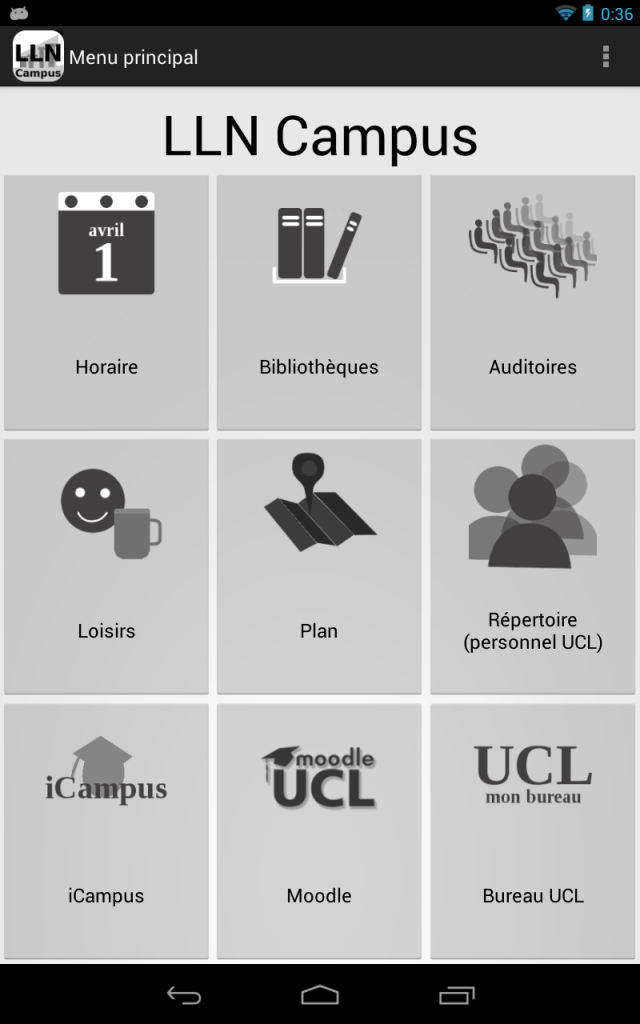
\includegraphics[scale = 0.2]{Images/llncampus.png}
\caption{LLN Campus home menu}
\end{figure}

\newpage

\subsubsection{LLN Maps}
LLN Maps is an application showing maps of Louvain-La-Neuve with relevant information and is developed by researchers of the Louvain School of Management. It is implemented using the Ionic framework. It contains various information such as the locations of lecture halls, libraries or train stations. This information is available as markers on a map. A GPS guidance with time calculation is possible from the user's position to each points of interest. There is a search bar if a specific information is required. Moreover a compass mode is available. See figure 2.3 for a visual.


\begin{figure}[H]
\centering
\begin{subfigure}{.5\textwidth}
  \centering
  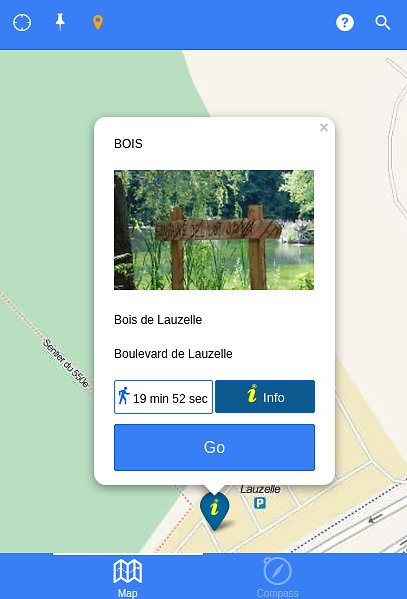
\includegraphics[width=.6\linewidth]{Images/llnmaps1.jpg}
  \label{fig:sub1}
\end{subfigure}%
\begin{subfigure}{.5\textwidth}
  \centering
  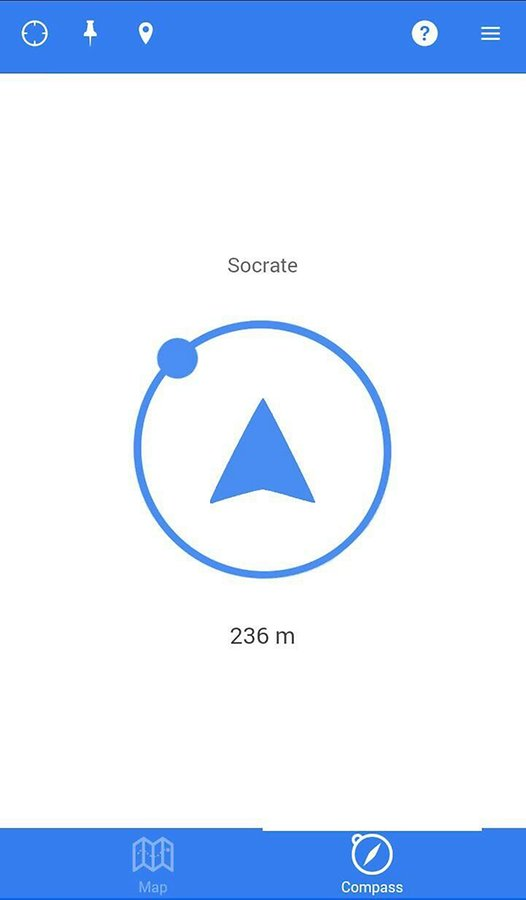
\includegraphics[width=.55\linewidth]{Images/llnmaps2.jpg}
  \label{fig:sub2}
\end{subfigure}
\caption{LLN maps}
\label{fig:test}
\end{figure}
We contacted the researchers that implemented the LLN Maps application and asked them to integrate their application into ours as outside contributors. Integration was made easier by the fact that both projects use the same framework.



\subsubsection{Quivr}
Quivr \footnote{\url{https://quivr.be/home/}} is the application developed by the Katholieke Universiteit Leuven. It is not open-source. This application is developed by 22 members and has over 60 000 users. It has a lot of features and it takes into account all KUL sites, not only Leuven. The different features are a schedule, a friend system, libraries, cafeterias and news. The list of features is impressive but the lack of available source code made it impossible for us to use this application as a basis for ours in any way.


\section{Project Management Methodologies}

Here we detail the choices we made as to how we were going to manage the different parts of the project. We worked with an agile approach with a sprint system. 

\newpage

\subsection{Agile Development}
An agile method has a good compatibility with the project. Agile development is based on different principles, the most interesting in our case are:

\begin{itemize}
\item A fast and continuous delivery to the customer, fast feedback.
\item Flexible requirements, even in development.
\item Weekly delivery rather than monthly.
\end{itemize}

\subsection{The Project Step By Step}

Firstly, the steps required before the project implementation:
\begin{enumerate}
\item Define the functionalities of the application. These functionalities are defined under the form of user stories. For example, "As a student, I want to be able to export my ADE schedule into my agenda". The details of this step are in section 3.1.
\item Create the application frames. An application preview allows us to discuss the functionalities and the design with people that are not related to the project. The details can be found in section 3.2.
\item Think about an architecture. The code should be easy to maintain, learn and handle. The architecture is explained in chapter 4..1
\item Create tasks from user stories. Each task has complexity points. Most of the time, the higher the complexity is, the more time it takes.
\item Initialize the task board.\\
\end{enumerate}

During the development, the process is :

\begin{enumerate}
\item Create a new milestone. A milestone defines a date for which a set of tasks should be done.
\item Select the tasks to do for this milestone. 
\item At the milestone date, analyse the work done and return to point 1. The analysis consists in summing the weight of each task the team was able to accomplish during the milestone. This sum represents the team velocity. This is useful for the next iteration, it allows to select a right number of tasks with a weight equals to this velocity.
\end{enumerate}

\subsection{ZenHub}
ZenHub is a GitHub extension. It is integrated in the GitHub interface and add functionalities such as a task board and a velocity management.  

\subsubsection{Create A Task}
One of the strengths of ZenHub is that it allows to transform an issue into a task. Figure 2.4 show the creation of an issue, it takes the following parameters:
\begin{itemize}
\item A title
\item A description
\item A pipeline. It is the column name of the dashboard where the task will be.
\item A label. Example, a bug, a question,...
\item A milestone.
\item An estimate. It is a value representing the task complexity.
\item Assignees. It assigns one or more developer(s) to the task.
\end{itemize}

\begin{figure}[H]
\centering
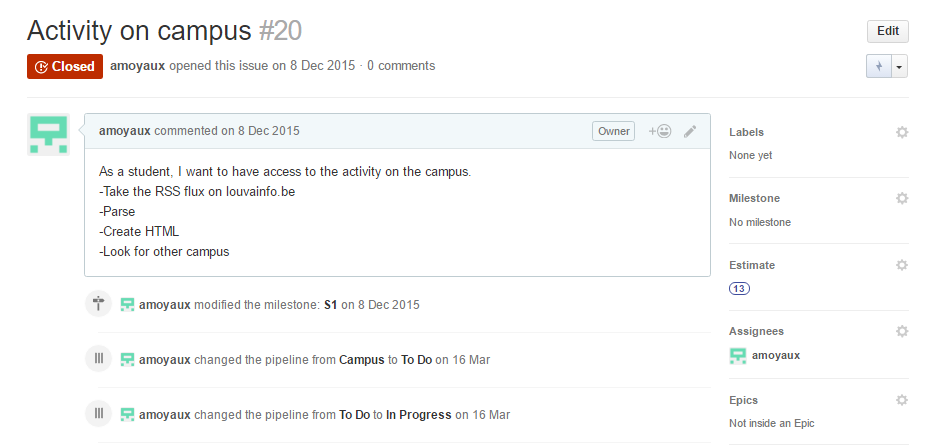
\includegraphics[scale = .65]{Images/issue.png}
\caption{Issue details}
\end{figure}

\subsubsection{Task Board}
Figure 2.5 shows the UCLCampus board. It contains the following columns:
\begin{itemize}
\item Student. All the tasks relative to the student section. This section only contains the tasks that are not done and that are not in the current milestone.
\item Campus. Same as student but for the tasks relative to the campus section.
\item Tools. Same as student but for the tasks relative to the tools section.
\item City. Same as student but for the tasks relative to the city section.
\item To Do. The tasks to finish for the current milestone.
\item In Progress. The task that are currently in progress.
\item Done. The finished tasks during the current milestone.
\item Closed. All the tasks done during the past milestones.
\end{itemize}

\begin{figure}[H]
\centering
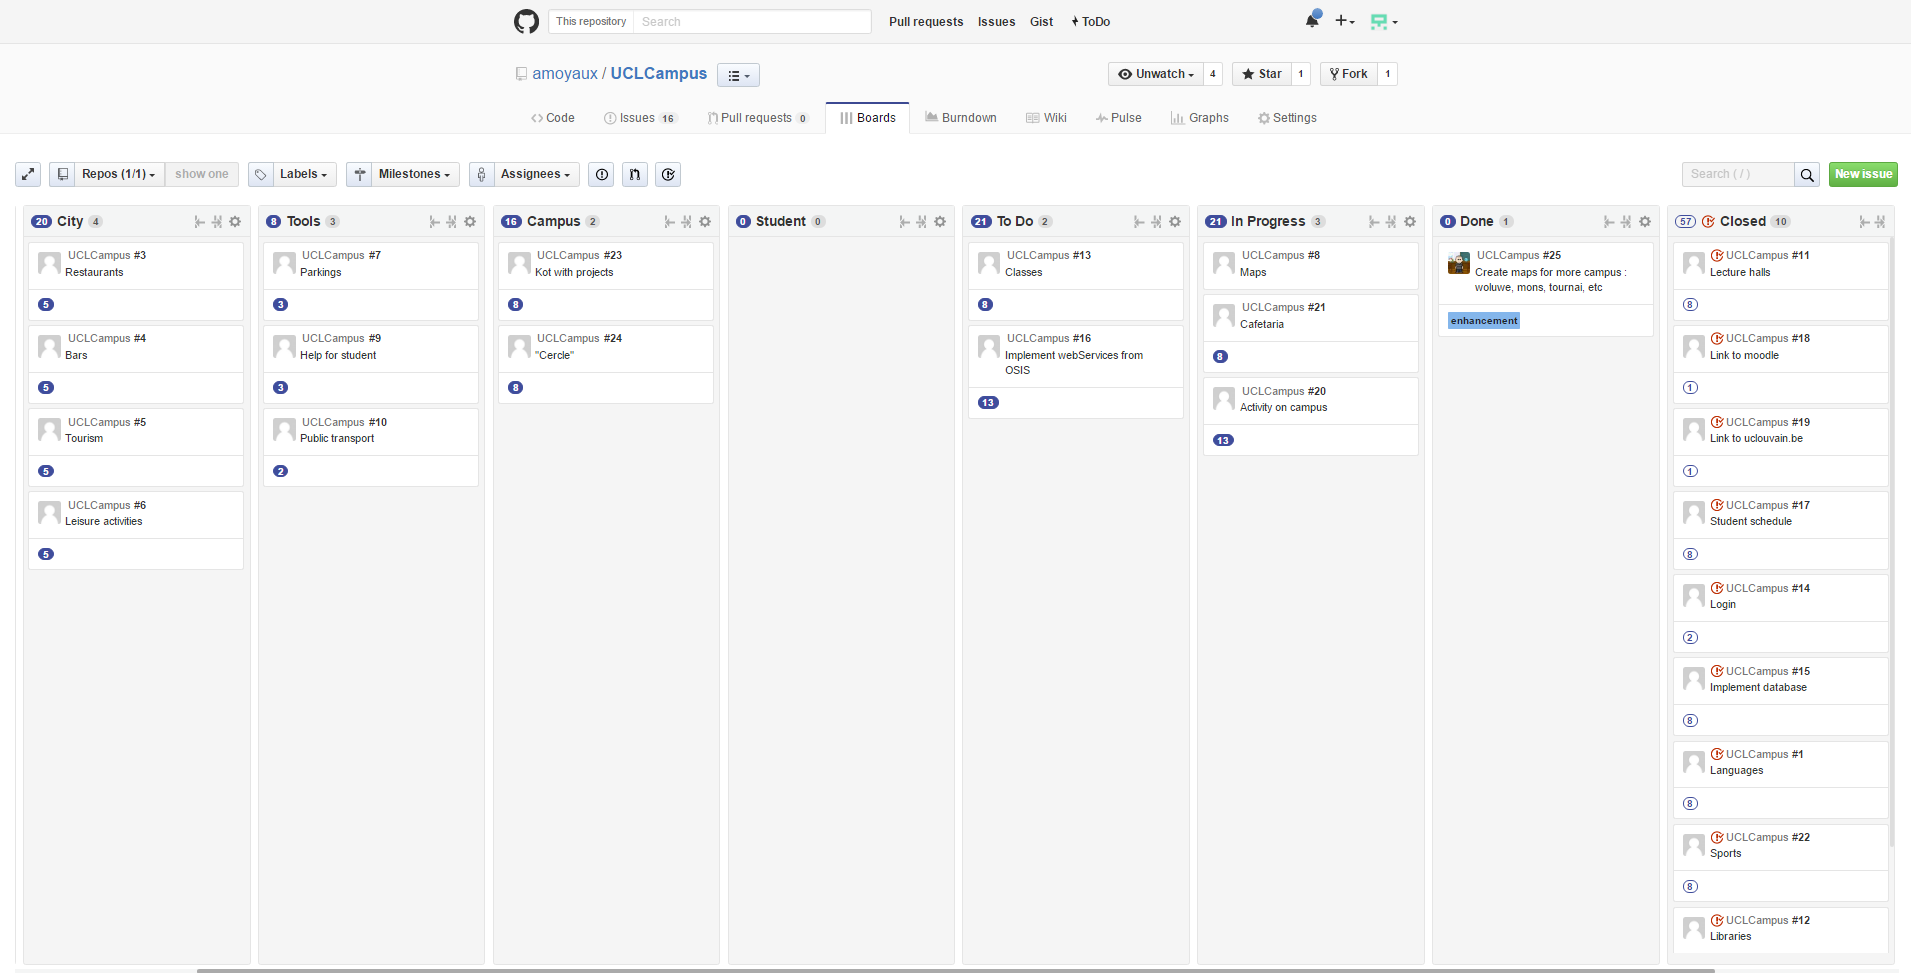
\includegraphics[scale = 0.45, angle = 90]{Images/dashboard.png}
\caption{Tasks board}
\end{figure}

\subsubsection{Milestone}

The milestone creation take three parameters:
\begin{itemize}
\item A title
\item A starting date
\item An end date
\end{itemize} 
To put a task in a given milestone, select the issue and set the milestone parameter on it. The milestone menu provides the list of tasks to do for the deadline. It provides an analysis about complexity point.

\chapter{Functionalities of UCLCampus}

Now that the background has been set and that we have made our initial choices, the next step is to define what the application will actually do. The first section of this chapter describes our thought process when choosing the different functionalities of the appliction while the second section explains our reasoning when defining the user interface.

\section{Choice of functionalities and sections}


In order to define what kind of functionalities would be part of our application, we needed to know what the students needed. The first step was to define a number of user stories that we would then translate into functionalities.\\ 
The user stories were split into several categories:

\begin{itemize}

\item Studies: anything directly related to a user's studies, for instance his classes, the lecture halls or the libraries.
\item Campus: anything related to student life in the campus but not related to the user's studies. For instance "Kot à Projets" or "Cercles".
\item City: anything related to the city the user is in but not related to the university. For instance a cinema or restaurants.
\item Tools: the tools offered by the application that might relate to several other categories. For example the map.
\item Settings: the settings of the application. For example the language or the currently selected campus.

\end{itemize}

We also define two types of users:

\begin{itemize}

\item Students: students can access all the functionalities of the application using their UCL login information. Indeed, some functionalities are student specific. For instance, it wouldn't make sense for a person who isn't a student to try to access his or her schedule.

\item Users: users are people who aren't students but might still be interested in some functionalities the application has to offer. 

\end{itemize}

In our user stories, any story starting by 'as a student' cannot be used by users while any story starting by 'as a user' can be used by both users and students.\\

We will now give a list of the different user stories we thought of for each of our categories.

\subsubsection{Studies}

\begin{itemize}

\item Schedule
\begin{itemize}
\item As a student, I can access my schedule in order to know when my courses are given.
\item As a student, I want to know where a course is given.
\item As a student, I want to know the name of a teacher giving a certain course of my schedule.
\item As a student, I can export my schedule to my phone's agenda so that I don't need Internet access to see it.
\end{itemize}

\item Libraries
\begin{itemize}
\item As a user, I can see whether a library is open or closed.
\item As a user, I can display the address of any library.
\item As a user, I can have a GPS guide to access libraries from my location.
\end{itemize}

\item Lecture halls
\begin{itemize}
\item As a user, I can check the address of any lecture hall.
\item As a user, I can have a GPS guide to access lecture halls from my location.
\end{itemize}

\item Websites
\begin{itemize}
\item As a user, I can quickly access the moodle website through the application.
\item As a user, I can quickly access the UCL website through the application.
\end{itemize}

\end{itemize}

\subsubsection{Campus}

\begin{itemize}

\item{Events}
\begin{itemize} 
\item As a user, I can see a list of events taking place in my campus.
\item As a user, I can sort the events by category.
\end{itemize}

\item{Kots à Projet}
\begin{itemize}
\item As a user, I can check Kots à Projet to know their address and projects.
\item As a user, I can have a GPS guide to access Kots à Projet from my location.
\end{itemize}

\item{Cercles}
\begin{itemize}
\item As a user, I can check "Cercles" to know their address.
\item As a user, I can have a GPS guide to access "Cercles" from my location.
\end{itemize}

\item{Cafeteria}
\begin{itemize}
\item As a user, I can see the different Cafeteria in my campus.
\item As a user, I can check the menu of the Cafeteria.
\item As a user, I can have a GPS guide to access Cafeterias from my location.
\end{itemize}

\item{Sports}
\begin{itemize}
\item As a user, I can see a list of sports organized in my campus.
\item As a user, I can sort the sports by day or by sport.
\end{itemize}

\end{itemize}

\subsubsection{City}

\begin{itemize}

\item Tourism
\begin{itemize} 
\item As a user, I can see the address of the city's information center.
\item As a user, I can see a list of the museums of the city I'm in.
\item As a user, I can see whether a museum is opened or closed.
\end{itemize}

\item Activities
\begin{itemize} 
\item As a user, I can see the address of the city's cinema in order to access it with the help of a GPS guide.
\item As a user, I can see several activities I can do in the city I'm in.

\end{itemize}

\item Restaurants and bars
\begin{itemize} 
\item As a user, I can see a list of the restaurants of the city I'm in.
\item As a user, I can see a list of the bars of the city I'm in.
\end{itemize}

\end{itemize}

\subsubsection{Tools}

\begin{itemize}
\item Maps
\begin{itemize}
\item As a user, I can access a map of the city I'm in in order to check points of interests.
\item As a user, I can receive help from a GPS guide in order to access a location of my choice on the map.
\end{itemize}
\item Mail
\begin{itemize}
\item As a student, I can check my emails on my uclouvain account.
\item As a student, I can send emails from my uclouvain account.
\end{itemize}
\item{Help}
\begin{itemize}
\item As a user, I can see where the UCL parkings are located.
\item As a user, I can receive help about how to configure the UCL wifi.
\item As a user, I can receive help about common transportation.
\end{itemize}
\end{itemize}

\subsubsection{Settings}

\begin{itemize}
\item As a user, I can change the application's language to French, English or Dutch.
\item As a user, I can select my campus.
\item As a student, I can login on my UCLouvain.be account.
\item As a student, I can log out from my UCLouvain.be account. 
\end{itemize}

\section{User interface}

Once we determined the different features we wanted in our application, we needed to organize them in a way that makes sense for users. In order to do so, we made sketches of what the application might look like using InVision. InVision is a website that lets people design and style mobile applications prototypes. It allows us to get an idea of what the finished product might look like without having to dive into any code. The sketches we made are available in the annex.\\

In these sketches, we can see that we decided to have one menu per category we defined in the previous section. Each menu has an associated color, allowing the user to always have visual clues to help them know where they are.\\

Once the sketches were done, we shared the link to our prototype to over 1000 students, mostly student in their first year, as they represent the future users of this application. They were able to browse through the application using the buttons, as if it was already working, and leave comments and feedback wherever they wanted to.\\

While we didn't receive as much feedback as we would have hoped, the one we received was constructive and helpful. Most people were satisfied with our 3 first categories, Studies, Campus and City. The fourth category, however, was more criticized. Here are some comments we received concerning the Tools category.\\


\say{[...] \\ 
 Quelques remarques:
 \begin{itemize}
 \item L'icône "Outils" du menu principal pourrait être renommer par soucis de clarté, on s'attend à tomber sur les "outils" ou paramètres de l'application et non pas du campus/ de la ville.
 \item Je ne vois pas trop l’intérêt de l'onglet mail étant donné que la plupart des étudiants possédant un smartphone ont déjà leur boite mail étudiant connectée. 
 \item L'onglet "Aide" est un peu caché et on ne s'attend pas à trouver ces infos là quand on clique, le lien parking devrait plutôt figurer dans le menu "ville" par exemple. (le renommer "infos utiles", ou qqch de plus parlant que "aide" éventuellement).
 \end{itemize}
 [...]}\\\\

This first comment mostly points out that the "Tools" section lacks clarity and that the functionalities we can find in this section are either unclear or useless. Another comment shared the same sentiment:\\

 \say{[...] 2. la partie "mails" est sans intérêt puisqu'on est sur un smartphone où la messagerie est probablement déjà configurée.\\
 3. le menu "Aide" pourrait alors remonter d'un niveau et remplacer "Outils" qui n'est d'ailleurs pas très parlant comme titre de menu}\\

This comment also points out that the "Tools" section should either be renamed or that it should contain other functionalities. Both commenters agree that the mail section does not have its place in the application.\\

\newpage

After reading these comments, we decided to rework the Tools section. We agreed that the mail part was superfluous and we decided to drop it entirely. We also decided to drop the "Help" section as we didn't think it was important enough. That left us with the map. We decided that it was important that the map was not grouped with the city, the studies or the campus as it was important to all three sections. We thus decided to leave it in the Tools section. We also decided against renaming the section "Maps" as future contributors may very well add functionalities we didn't think of in this section.

\chapter{Implementation}

Once we had a clear idea of what the application was going to look like, we were ready to start implementing it. We started by designing a high-level view of the program which is detailed in the "Architecture" section 

\section{Architecture}

The purpose of the application is to be extensible and easily maintainable. A programmer needs to have the possibility to add his own functionalities at each level of the application.\\
The UCLCampus architecture can be seen as a tree. At the top level there are the generic parts and configurations that will be present everywhere in the application. Under it there are the settings menu and four other nodes representing the global sections. These sections are pointing to their functionalities and so on. Here is a part of the tree.\\

\begin{figure}[H]
\centering
\begin{forest}
[Application, for tree = {ellipse, draw}, fill = green
	[Settings]
	[Studies]
	[Campus
		[Events]
		[Cafeteria
			[Cafeteria details
				[Templates]
				[JavaScript]			
			]
			[Templates]
			[JavaScript]
		]
		[Cercles]
		[Sports]
	]
	[Tools]
	[City]
]
\end{forest}
\caption{Tree Architecture} 
\end{figure}

\subsection{Folder organization}
To be consistent with our architecture, the folders and files organization also follows a tree structure. Ionic base architecture is to group all html file in a folder named templates, all JavaScropt files in a JS folder and so on. This design becomes messy once there are a lot of functionalities and a lot of files. We modify it to respect the same tree structure described in the previous section. This folder organization allows programmers to efficiently find the code they need. For example, if a programmer wants to change the Cafeteria details user interface, he can follow the logical path Campus/Cafeteria/Cafeteria Details/templates. This folder path follows the tree implementation as seen on figure 4.1. Figure 4.2 is a summary of the changes we made to the basic Ionic design. Red folders are those that have been modified.\\ 
\begin{figure}[H]
\centering
\begin{subfigure}[b]{0.5\textwidth}
   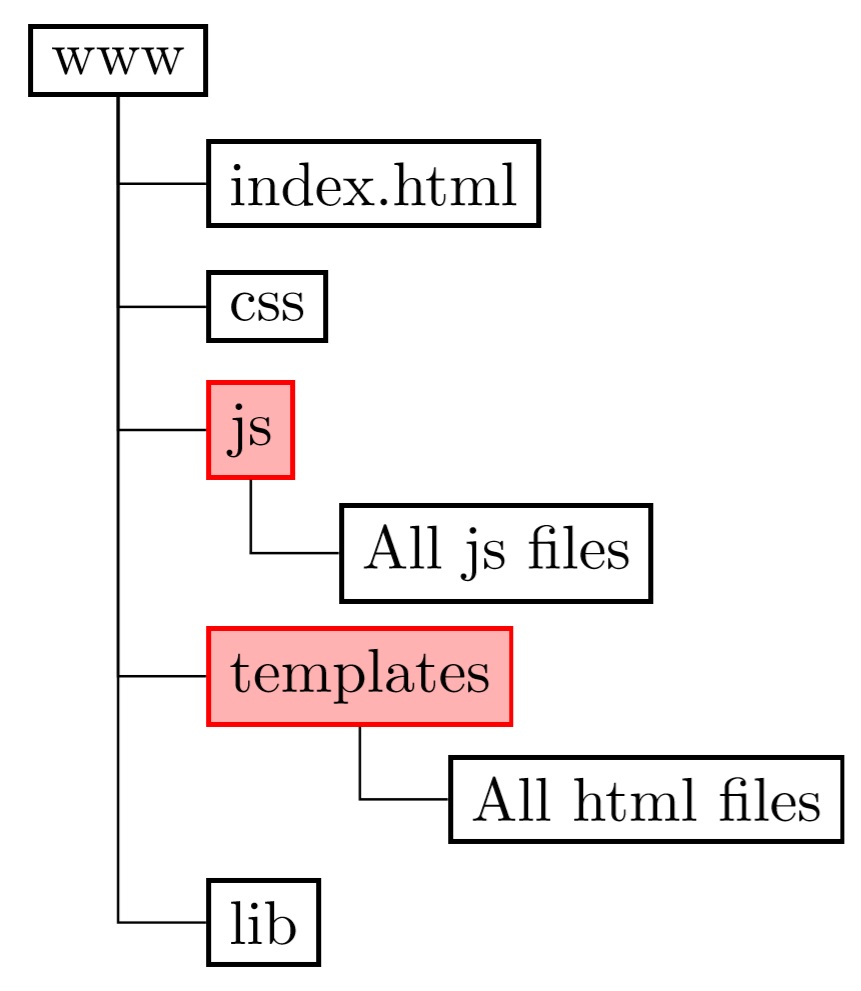
\includegraphics[width=.4\linewidth]{Images/folder_before.jpg}
  \caption{Before}
  \label{fig:before}
\end{subfigure}%
\begin{subfigure}[b]{.5\textwidth}
  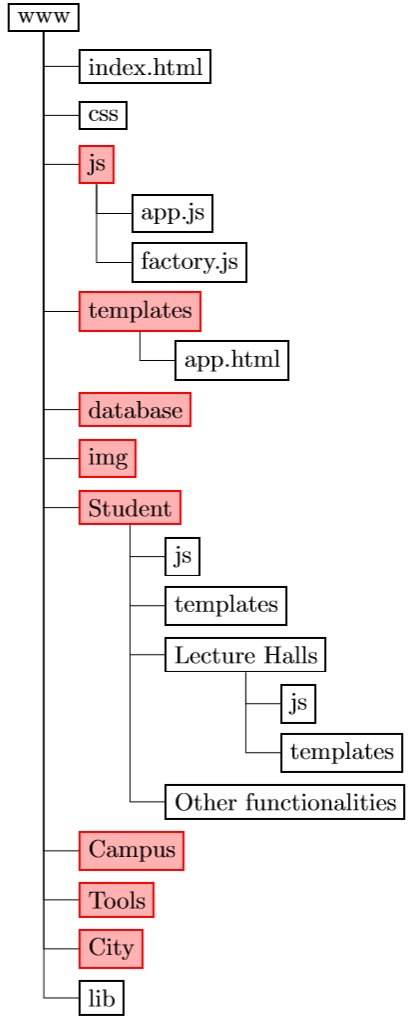
\includegraphics[width=.4\linewidth]{Images/folder_after.jpg}
  \caption{After}
  \label{fig:sub2}
\end{subfigure}
\caption{Folder evolution}
\label{fig:test}
\end{figure}

\subsection{Information processing}

This section explains how to deal with information processing from an architectural point of view. The section 4.4 explains in details how each specific part is implemented.
There is a lot of information to relay into the application (libraries schedule, libraries addresses, daily events in the campus,...). There are three ways to import them. The first way is to use a database, the information are encoded in tabular form and it can be retrieve using queries. The two other methods are web parsing and web services. Web services are always better than web parsing. Web services consist in sending a request to a server and receiving a response that contains exactly the information needed. Web parsing is sending a request to a server but there is a need to search for the information inside the response.\\

In an ideal scenario, static information would only be retrieved via a local database whereas frequently updated information could be retrieved using web services. However, such databases and web services are not always available. This means that he three methods are used in the application depending on the available service.
\\ For example, the ADE schedule has no web service. We therefore need to either use web parsing or store the information in a database. Encoding the schedule for all students in the database requires 80Mo of memory space, which is more than the actual application size and is too much for a mobile application. In this case, web parsing seems to be the right choice.\\  Another example is the events. Events are updated daily. If we were to store such events in a database, we would need a developer to update said database daily. In this case however, the events are available through a RSS flux, meaning we don't need to parse the website to retrieve them.

The following figures detail the pros and cons of each of these 3 approaches.

\subsubsection{Database}

\begin{table}[H]
\begin{tabularx}{\linewidth}{>{\parskip1ex}X@{\kern4\tabcolsep}>{\parskip1ex}X}
\toprule
\hfil\bfseries Pros
&
\hfil\bfseries Cons
\\\cmidrule(r{3\tabcolsep}){1-1}\cmidrule(l{-\tabcolsep}){2-2}

Always available\par
Easy information retrieval(query)\par
Easy to modify\par
Fast\par

&

Need human resources to update information\par
Takes memory \par


\\\bottomrule
\end{tabularx}
\caption{Pros and cons of a database}
\end{table}

\subsubsection{Web Services}

\begin{table}[H]
\begin{tabularx}{\linewidth}{>{\parskip1ex}X@{\kern4\tabcolsep}>{\parskip1ex}X}
\toprule
\hfil\bfseries Pros
&
\hfil\bfseries Cons
\\\cmidrule(r{3\tabcolsep}){1-1}\cmidrule(l{-\tabcolsep}){2-2}

Automatic update\par
Easy information retrieval with query\par
No hardware memory consumption\par

&

Need an Internet connexion and an operational server side\par
Impossible if not implemented on the server\par

\\\bottomrule
\end{tabularx}
\caption{Pros and cons of the web services}
\end{table}

\subsubsection{Web Parsing}

\begin{table}[H]
\begin{tabularx}{\linewidth}{>{\parskip1ex}X@{\kern4\tabcolsep}>{\parskip1ex}X}
\toprule
\hfil\bfseries Pros
&
\hfil\bfseries Cons
\\\cmidrule(r{3\tabcolsep}){1-1}\cmidrule(l{-\tabcolsep}){2-2}

Automatic update\par
No hardware memory consumption\par

&

Need an Internet connexion and an operational server side\par
Need one more step than web services. This step is to find the required data inside the server response\par
If the web server change its response, the parsing method also needs to be modified\par
Slow compared to web services and database\par


\\\bottomrule
\end{tabularx}
\caption{Pros and cons of the web parsing}
\end{table}

\newpage
\subsection{Front end and back end}

The application is split into two main parts:
\begin{itemize}
\item The front end: The front end is the interface between the user and the back end. It can either design the graphical user interface or the methods implemented to give programmers access to data regardless of the way they are retrieved.
\item The back end: Everything that is not part of user interface. Storage system, information retrieval, ....
\end{itemize}

The UCLCampus architecture contains a back end/front end system. Such a system makes the application more modular. For a functionality, the code for the user interface is totally isolated from the code for storage. This means that it is possible to change a user interface without seeing the code for storage. Inversely, it is possible to change the code for the storage without touching the user interface.\\
For example, it is possible to pass from a database storage to a web parsing for libraries without this change having an impact on the user interface methods.

\subsection{Factory}

A factory is a functionality from AngularJS that we used as a back end service. The factory will take the data from the database or web parsing, modify the data format to be easier to handle and then transmit it to the front end. Figure 4.3 illustrates this.\\

\begin{figure}[H]
\centering
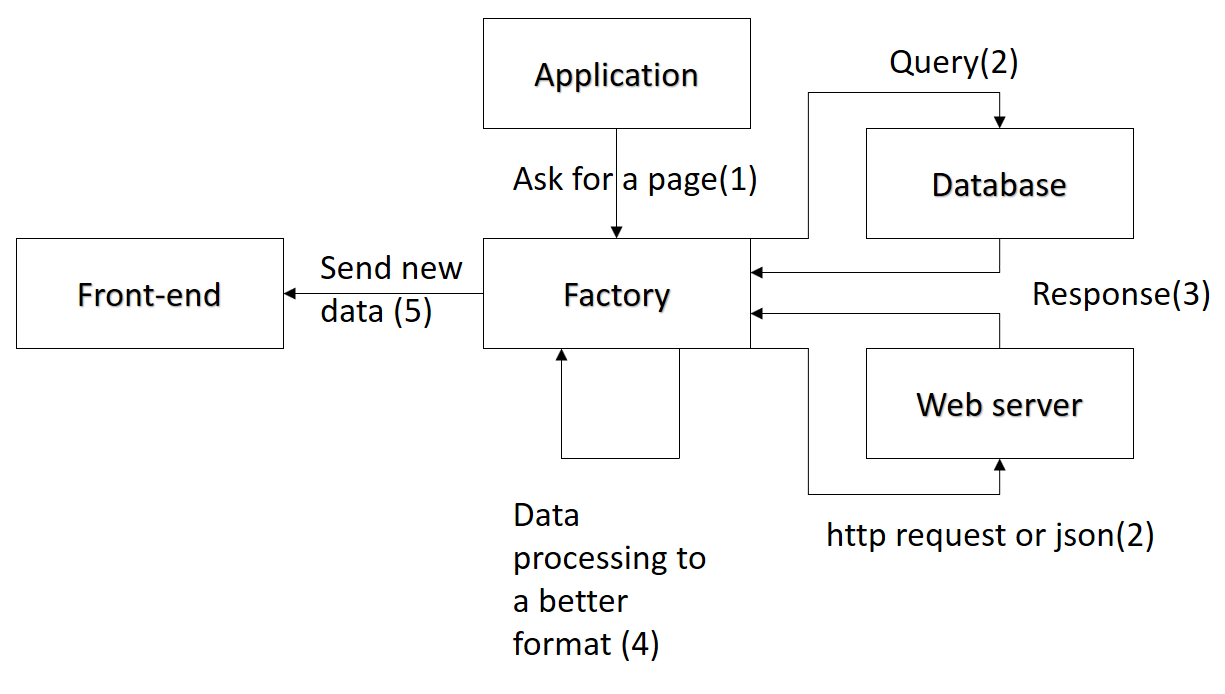
\includegraphics[scale = 0.3]{Images/factory_arch.png}
\caption{Factory operation}
\end{figure}

For instance, the steps explained in figure 4.3 would result in the following behavior if we wanted to retrieve a student's schedule via ADE.

\begin{enumerate}
\item The system notifies the schedule factory in order to get the required data.
\item The factory create a custom HTTP request and send it to the ADE domain.
\item The ADE server sends a response.
\item The data found in the response is not easy to manipulate (long string with html tags inside), so the factory picks the important elements in the response and puts them in a JavaScript object which is easier to handle.
\item Send new data to the front end.\\
\end{enumerate}

\subsection{State provider}

The state provider is a functionality of AngularJS. It allows to define some options for the different views of the application. It can, for instance, be used to define whether a given view should be cached or not. Furthermore it creates an edge between the back end and the front end. Figure 4.4 illustrates the operations of the state provider. 
\begin{figure}[H]
\centering
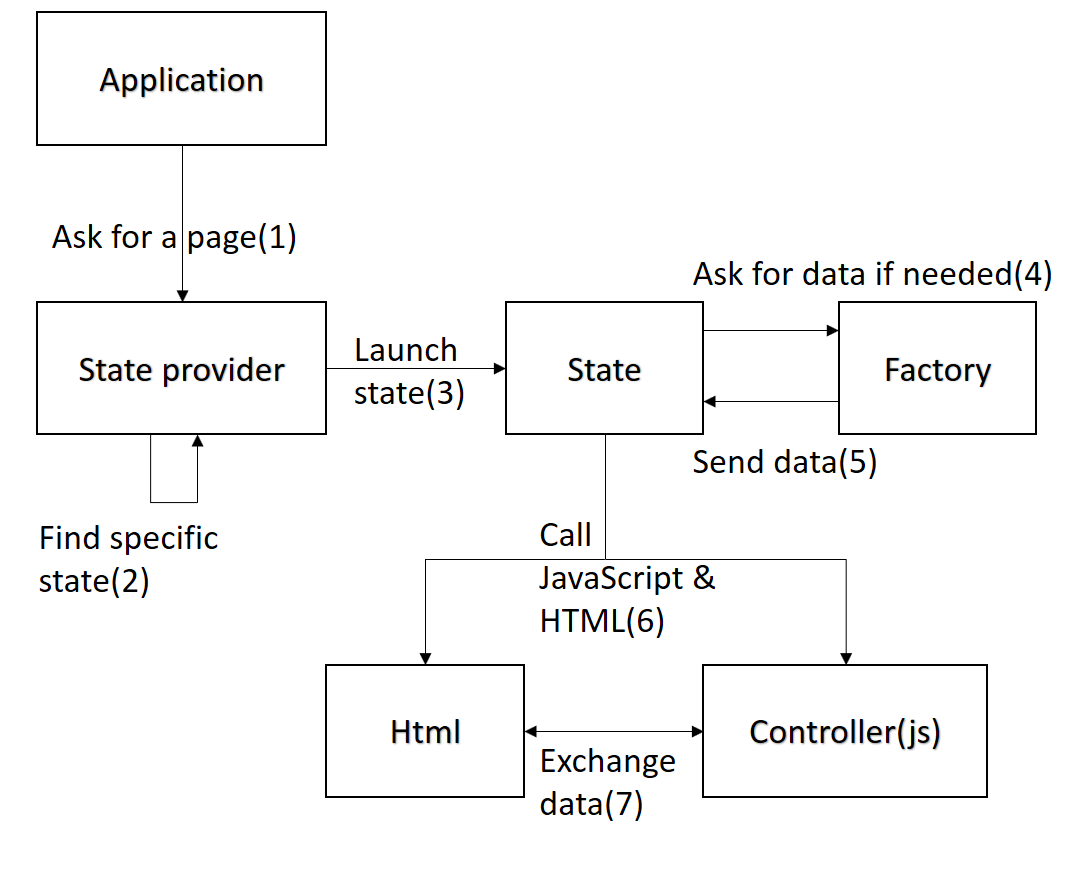
\includegraphics[scale = 0.3]{Images/stateProvider_arch.png}
\caption{State provider operation}
\end{figure}
First the application asks for a page. The state provider contains a list of specific states (one state by page), it will then return the state relative to the asked page. The state will contain information about the page:
\begin{itemize}
\item The location of the HTML template
\item The associate controller(JavaScript)
\item A flag for cached memory (true or false)
\item The section membership (for example student if we are in the student tab)
\end{itemize}. If the state needs to access data through the back end, the state will call the needed factory and wait for its response before launching the template and the controller for the user interface. The following snippet gives an example of a state as seen in the state provider.


\begin{lstlisting}
.state('app.name', {
    cache:{true or false},
    url: "/url name",
    views: {
      'appropriate-tab': {
        templateUrl: "html file",
        controller: "page controller(javaScript)",
        resolve:{
          factory: function(Factory) {
            return Factory.neededData();
          }
        }
      }
    }
  })
\end{lstlisting}

We can see that every information needed is shown in this snippet. We start by giving the state a name. We will use this name to start the state. We then define whether the corresponding view should be cached or not. Then, we define the url of the state.

The views field contains the tab the view is located in as well as the location of the template (HTML file) and controller (JavaScript file).
The resolve is only used if we need to access data from the back end. 

\section{Coding standards}

This section defines a few standards we established when adding functionalities to the application. 

\subsection{Header and footer}
We managed our code to automatically create a new default footer and header when you start new HTML template. The footer and header have a specific color for each tab-section (blue for student, yellow for campus, purple for tools and green for town). We allow developers to overwrite the default header but under two conditions:
\begin{itemize}
\item The title has to keep the same font and has to be centered.
\item The header color must respect the section color.
\end{itemize}
Footers must not be overwritten or hidden. If developers need to insert their specific header or footer, Ionic provides a CSS in order to add subfooters and subheaders.
\subsection{Tree hierarchy}
We want developers to keep the tree hierarchy we created for the state and for the folders. 
\subsection{Colors}
We used the UCL color code\footnote{https://www.uclouvain.be/459461.html}. For this we modified the sass theme of Ionic. This allows modules developed with basic ionic CSS component to use the application's colors instantly and automatically.

\begin{center}
    \begin{tabular}{ | c | c | c |}
    \hline
    Color & CSS name & Code\\ \hline
    Blue & positive & \#00214e\\ \hline
    Yellow & energized & \#f29400\\ \hline
    Purple & royal & \#88005d\\ \hline
    Green & balanced & \#76ad1c\\ \hline
    \end{tabular}
\end{center}

\section{Security}

Most of the application's features don't need an additional security layer on the application's end as they only consist in parsing publicly available web pages or accessing publicly available databases. It is however important to secure the data retrieved from the uclouvain.be website concerning a student's classes. This information is indeed not publicly available. However, this functionality was not implemented in the current version of the application for reasons detailed in the next chapter. We however looked at ways we could make sure no data is accessible by anyone else than the student himself.

\subsubsection{Data to protect}

The data we need to secure consists of several things:

\begin{itemize}
\item The student's credentials
\item The student's classes
\item The database of all students' classes
\end{itemize}

\subsubsection{Possible threats}
A person other than the student might try to access the aforementioned data in two different ways. The first way to access the data is through the student's phone, by looking in the local storage. The second way is to inspect the packages sent by the application to the OSIS server and vice-versa. 

\subsubsection{Protections}
For the first threat, the password and the username should not be stored on the device (even if they are encrypted). So the solution to this problem would be to create the OSIS request directly when the user inserts his credentials. With this procedure, we only store the student classes list and forget the credentials once the request is sent. The courses list should not be accessible by an other person than the user but it is less critical than credentials, so in this case, it should be encrypted on the local device. \\

For the second threat, a solution would be to create a secure connexion with OSIS where packets are encrypted. For example an RSA encryption with public and secret key, UCLCampus would send a first request to obtain a public key from OSIS, encrypt the request with it, send it back to OSIS that can decrypt it with the secret key. Due to this procedure, the person trying to access the data can catch the packets between OSIS and UCLCampus but can't read or do anything with them.
\section{Information retrieval}

In this section we will detail the different sources of information we used in our application as well as the technologies we had to use in order to retrieve said information. 
\subsection{Student data(OSIS)}

OSIS web serviceshave not yet been implemented but would be implemented in the following way. The SGSI replies to our request with a JSON file that has the following structure:

\begin{verbatim}
Student[{
    registration_id
    FirstName
    LastName
    Offers:[{
        Acronym
        Title
        Learning_unit:[{
            Acronym
            Title
            Credits},
        {...},...]
    },{..},...]
}]
\end{verbatim}
This represents a student with a first name, last name and a registration id. The offers represent a learning option. Example, BAC1 in computer science. A learning unit represent a course. \\

We create a query with the student username and password as parameters to obtain this response. The response can be automatically transformed from this JSON format to a JavaScript object. The JavaScript is stored and used in other functionalities.\\

If the username and password in the query don't match any student, the server returns an empty response. 



\subsection{Libraries and lecture halls}

In order to retrieve a list of all libraries and lecture halls in the university, we contacted the UCL to ask them if such a database existed. Sadly, it appeared that no database of this kind exists. We then wondered how LLNCampus managed to obtain all the information they had on lecture halls and libraries. Since their application is also open-source, we were able to find the database they used. Since it was very complete and was the only database available, we decided to re-use this database. However, since their database was built with only one campus in mind, we had to change it a bit.

\subsubsection{Database structure}
 
The database is an SQLite database. The table we use for the most part is called "poi" (point of interest) and has the following fields:

\begin{itemize}
\item ID (integer): used to identify the item
\item Name (text): name of the point of interest
\item Latitude (real): latitude of the point of interest
\item Longitude (real): longitude of the point of interest
\item Type (text): type of the point of interest, can be "auditoire", "kap",   "bibliotheque", ...
\item Address (text): address of the point of interest
\item Img (text): path to the image linked to the poi
\end{itemize}

To these fields we added the following two:
\begin{itemize}
\item Campus (text): campus where the poi is located
\item Abbr (text): abbreviated version of the poi. For instance "BARB" for the Ste-Barbe lecture hall
\end{itemize}

The first field is useful if we want to have different campuses while the second is used to find the poi on the map.

\subsubsection{Retrieving lecture halls}

Once we had completed the database, we had to connect it to our application. In order to do so, we used the cordovaSQLite plugin. Once connected, we were able to retrieve the lecture halls using the following SQL query: 
\begin{verbatim}
SELECT * FROM poi WHERE TYPE = 'auditoire' AND CAMPUS = ?
\end{verbatim}

This query will retrieve all the fields from the poi table we discussed earlier which have the type "auditoire" and are located in the desired campus. The "?" character is used as a placeholder for an argument we can pass to the function. We will then store the result of the query in a JavaScript array and used that array to display the information to the user.

\subsubsection{Retrieving libraries}

In order to retrieve all the information concerning libraries, the poi table was not enough. Indeed, we wanted the users to be able to know whether a library was opened or closed and the schedule was not available in the poi table. Thankfully this information was available in another table, called "bibliotheque\textunderscore horaire". This table only has 4 fields:

\begin{itemize}
\item Building\textunderscore ID (integer): identifies the library. Same id as the one used in the poi table.
\item Day (integer): Day of the week (0 for monday, 1 for tuesday, ...)
\item Begin\textunderscore time (integer): Time of the day when the library opens. Given in minutes elapsed since midnight
\item End\textunderscore time (integer): Time of the day when the library closes. Given in minutes elapsed since midnight
\end{itemize}

Given this new table we were able to retrieve all the information we needed using the following SQL query:
\begin{verbatim}
SELECT * FROM poi, bibliotheque_horaire WHERE poi.TYPE = 'bibliotheque' 
AND poi.ID == bibliotheque_horaire.BUILDING_ID AND DAY = ? AND CAMPUS = ?
\end{verbatim}

This query retrieves all poi with type "bibliotheque" and finds their respective schedule for a given day, all that for a given campus. The result in then stored in a JavaScript array.

\subsection{Events}

In order to find events taking place in Louvain-la-Neuve, we used the www.louvainfo.be website. This website provides a schedule of all upcoming events in the city. It is however specific to Louvain-la-Neuve and we would need to find equivalent websites for the other campuses. \\ The website provides an Atom RSS feed of the events. We decided to use Yahoo Query Language to parse the RSS feed and retrieve the information. The reason we used the Yahoo Query language (YQL) was that it was the only way we found to perform such an operation. Indeed, the more widely used Google Feed API has been deprecated. We therefore had no other choice but thankfully we haven't encountered any issue with YQL.\\
\\We used the following query to retrieve the feed:
\begin{verbatim}
select * from feednormalizer where url='http://louvainfo.be/evenements/feed/calendar/'
\end{verbatim}
The result is then automatically parsed and stored in a JavaScript objects array. 

\subsection{Schedule}
For the schedule we had no choice but to use web parsing. The ADE dump database for all courses (of all the students) has a size of 80Mo which is way too much memory for a mobile application. Therefore ADE has a custom web site where you are able to send customized urls in order to extract specific informations. It's a bit worse than web services because you need to parse the response to retrieve the relevant information.
\subsubsection{ADE custom URL}
The request always starts with \url{http://horairev6.uclouvain.be/jsp/custom/modules/plannings/direct_planning.jsp?}. After this we can add some query parameters.
\begin{itemize}
\item Code : The course code we want to see on the schedule. The list of course acronyms used comes from the OSIS response. It is the list of acronyms for all leaning units in the current offer of the student. .
\item weeks : The weeks we want to see. It's a number per weeks. We wanted to get all the year so we used a list from 1 to 52 (1,2,3,...).
\item projectID : A number defining the academic year we want to see(16 for 2015-2016). This number needs to be manually updated each year. We couldn't update it automatically because it seems to be a random number chosen each year(7 and 16 for the last two years).
\end{itemize}

\subsubsection{Parsing}
The HTTP response contains an HTML code. It contains information about each lecture of the year. Here is the syntax of the table in the response.\\
<tbody>\\
\tab <tr>\\
\tab \tab <td>Date</td>\\
\tab \tab <td>Course Code</td>\\
\tab \tab <td>Hours:Minutes</td>\\
\tab \tab <td>Date</td>\\
\tab \tab <td></td>\\
\tab \tab <td>Useless information</td>\\
\tab \tab <td>Eleves</td>\\
\tab \tab <td>Professors</td>\\
\tab \tab <td>Place</td>\\
\tab \tab <td>Course Code again</td>\\
\tab </tr>\\
\tab <tr> Another lecture </tr>\\
\tab ...\\
</tbody>\\
We used a string parsing based on regular expression in order to extract information from tags and place it into a JavaScript object with field easily accessible. Once the parsing is done the back end sends a list of lecture objects to the front end.

\subsubsection{Local storage}
We thought it could be good to keep the schedule relative to the logged student in memory. In this case he could have an access to it every time without the need of an internet connexion. For this, once the parsing done, we keep the new schedule object in memory and the next time the student accesses the page we load it from local storage instead of parsing it again. This increases performances because it's faster and has a better availability. The problem is that the schedule can change during the year so we allow the student to force a new web request with a new parsing in order to update it (with a refresh button on the page).

\subsection{Cafeteria}
We chose to store the main informations (name, location, image, opening time) about restaurants in the database because it's  something that will not change every year and there is not a lot of field to update if some modifications are needed. We encode the 6 restaurants present on the UCL website\footnote{https://www.uclouvain.be/restaurants-universitaires.html}. For the database we created a new table and encoded data manually. The menus sadly couldn't be stored in the database because of the existence of the daily menu (we should omit them or update them manually each week). We wanted to do some web parsing but the html code for each restaurant had its own syntax and thus we would need to create one parsing technique by university canteen which was a too heavy workload for the time we had. Instead we chose to create a button linking to the related menu page.
\subsection{Sports}
We couldn't store the sports in a database because the planning undergoes changes every year and we don't have manpower to update it. The sports department doesn't have web services either so the only solution we had was to parse the website. On a positive note, the Louvain-la-Neuve and Woluwe sites share the same website and thus the parsing is effective for both. 
\subsubsection{URL}
The base URL for the two websites is the same \footnote{\url{http://ucl-fms01.sipr.ucl.ac.be:82/ucl_sport/recordlist.php?}}. There are two main query parameters possible:
\begin{itemize}
\item The campus: A number defining the campus for which we want to show the sports schedule(1 for all, 2 for Louvain-la-Neuve, 4 for Woluwe). The factory creates a specific request with 2 (resp.4) when the selected campus is Louvain-la-Neuve (Woluwe)
\item The skip: The sport web site response contains only 50 sports time slots. The skip argument allows to access the other sports instances after the first fifty.
\end{itemize}
It is a bit more difficult and slower than the other request because in this case we need to create a request by 50 sports time slots(for example if we have 132 sports we need three request. The first taking 0-50 instances, the second 51-100 and 101-132 for the last). Moreover the website is not always available, and we sometimes couldn't access it because it was offline so we added a time-out method in order to prevent the user from waiting indefinitely.
\subsubsection{Parsing}
For the parsing the sport has a similar structure than the schedule except it uses different tag names so we used another string parsing method based on regular expression. The sport website creates a page that contain the sport closer to the current day and the time. For example if today is Friday and it is 14 o'clock, it will show the Friday sports time slots after 14 o'clock first. Thus we iterate over all the time slots until we are sure that we capture all the sport for a week. We stocked the result in an other list of JavaScript object that we store and send to the front end.
\subsubsection{Local storage}
The reasoning here is the same as the one described in the schedule section above. Here we saved the result for both Louvain-la-Neuve and Woluwe in different tables so we have them both in memory once they has been accessed at least once. Moreover each time the page is requested the software will reorganize the list in order to have the closer time slots first which is in general more suitable for the user. 

\newpage

\chapter{The Application}

This section will detail the different functionalities we were able to implement in our final version of the application and will explain how to add a new functionality to future contributors. The chapter will end by explaining a series of test we implemented to make sure the implemented functionalities were working as intended. //TODO annexe

\section{The UCLCampus application}

\subsection{Header}
\paragraph{Design}
We created a global header for the application. The header has different colors depending on the section (Chap 4.2.3 for more details). Otherwise, it has three components. The first is the name of the page. For example "Sainte-Barbe" if we are looking at the details of this lecture hall. The two other components are buttons, the first is the back button, it allows to go back to the previous page. The second button open the settings menu. This header is by default enabled on all the pages of the application but the programmer can overwrite it if he wants to add something, such as new buttons, search bar,...
\paragraph{Implementation}
The Ionic framework provides a file named index.html in its architecture. This file has two purposes. The first is to list all the JavaScript present in the application in order to run them. The second is to create pieces of a user interface that will be available everywhere in the application. These pieces can be overwritten. We used it to create the header, the footer and the settings menu. It's a good point for the maintainability because here we have a single code for every header except if they have been overwritten. Thus it can be modified quickly and efficiently. 
\subsection{Footer}
\paragraph{Design}
The footer is a bar with buttons at the bottom of the screen. As the header, the footer color changes depending on the section. There are four buttons on the footer, corresponding to the four main sections (student, campus, tools, city). We thought it was more user-friendly to do that because you don't need to click on the previous page until you reach the main menu if you want to explore another section. For example, if you are looking at the details of a lecture hall and you want to see the events of the week, without footer you would need to click three times on the back button to reach the home menu then select campus and events, making it a total of five manipulations. With the footer, you can click on the campus button and then event, which is only two steps. 
\paragraph{Implementation}
Ionic provide all the components and an extended architecture for the tabs (buttons in the footer). When we create a page, we create a state associated with it (see chapter 4.1.5). In this state, we can set an argument specifying the section it belongs to. Once it is done, Ionic automatically manages the tabs function. 
For example, if we are on the libraries’ page, there exists a state associated with it, informing that this page belongs to the student section. From that, the framework manages automatically to highlight the student button in the footer in order to show the user that he is in the student section.
For more details\footnote{\url{http://ionicframework.com/docs/api/directive/ionNavView/}} see figure 5.1, it creates a tree structure of sections, or tabs in the schema. Each section holds a list of views (pages) and its own navigation history stack. The history stack matters for the back button function. 
\begin{figure}[H]
\centering
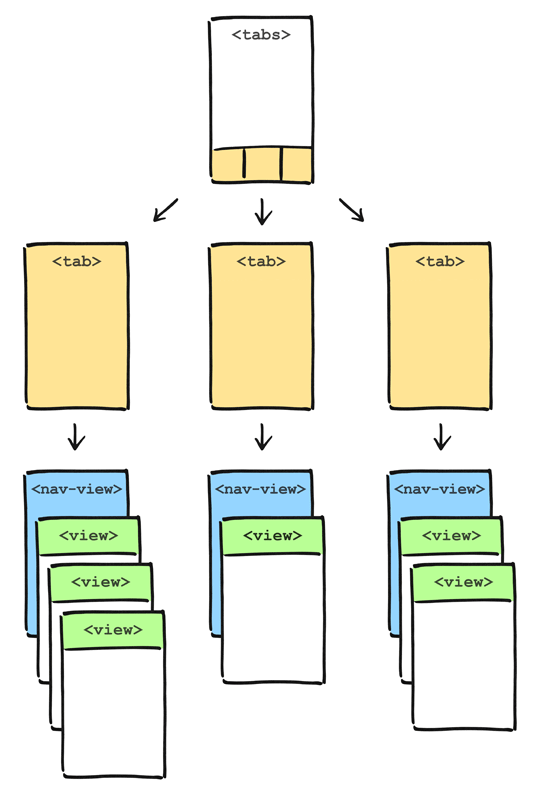
\includegraphics[scale = 0.3]{Images/tabs-nav-stack.png}
\caption{Tabs diagram}
\end{figure}

\subsection{The Homepage}
When the user launches UCLCampus on his smartphone, he arrives on the homepage. This page contains the header and four buttons(student, campus, tools, city). The purpose of this page is to not force the user to be in a menu once he opens the application. Another choice could be to put him in the student section and let him use the footer button to navigate between sub menus, we found this solution less comfortable for the user. We removed the footer from the homepage because it's redundant to have the sub menu buttons at the same time as the content of the page and in the footer.
\subsection{The Student/Campus/Tools/City Menus}
The four sub-menus have the same design and are implemented the same way.
TODO lien vers l'annexe des screens ou alors importer l'image. 
\paragraph{Design}
The menu offers a list of buttons. Each button has a corresponding functionality and a representative icon next to it.
\paragraph{Implementation}
The four menus have the same code skeleton. The principle is simple, each menu has his own factory. This factory holds a list of objects, each object represents a button. These buttons have different parameters: 
\begin{itemize}
\item Title: The name of the functionality the button is pointing to.
\item Icon: An icon representing the functionality.
\item URL: The technical link to the new page. If this is set, website parameter should be null.
\item Website: The application can open an external website, in this case this field is the URL. If this field is set, URL should be null.
\item Campus: A list of campuses where the functionality is implemented. For example, if we set it to ['Louvain-la-Neuve','Woluwe']. If the user's selected campus is one of these, he will see the button on the menu, if not the button is not present. The list can be empty([]), this case is equivalent to write all the campuses which is easier for the programmer. 
\end{itemize}
This list is then simply passed to the HTML and JavaScript controller that use it in order to create the user interface.
\subsection{Studies}
The student menu contains all information relevant to the academic year. All the functionality except libraries and lecture halls are available for every campus. We have libraries and lecture halls informations in database only for Louvain-la-Neuve and Woluwe. 
\subsubsection{Schedule}
For the schedule we didn't want to implement a fresh new calendar algorithm with a lot of functionalities because it's already present on all smartphone as native agenda. So the purpose of this section was allow the student to export their ADE schedule directly to their agenda. We nevertheless implemented a display function where the student can see the lectures he has for a selected day. In order to implement it we used the data send by the back end (explained in chap 4.4), we display this data as list with
\begin{itemize}
\item Time slot
\item Course code - Professor
\item Local
\end{itemize}
To only display the lecture for a selected day we create a JavaScript filter. In order to let the user select a day we used the onezone datepicker plugin(open-source, MIT license\footnote{\url{https://market.ionic.io/plugins/onezone-datepicker}}), it's just a date picker object that displays a calendar where you can select the day you want. Moreover, we implemented swipe right and swipe left functions in order to add or remove a day from the current date.
To export the list of lectures to the native calendar, we used the PhoneGap Calendar plugin \footnote{\url{https://github.com/EddyVerbruggen/Calendar-PhoneGap-Plugin}}(MIT). It allow us to create, remove and update events in the agenda. However this plugin is still in development and could create some issues, it should not be delivered to end users but we could not find a better solution. We add a button in the header to refresh the schedule if the student needs to. 

\subsubsection{Lecture Halls}
This functionality was implemented in two phases. The first state is an overview of all the halls. For this the controller calls the factory method a first time to have all the lecture halls in a list where we can access details efficiently (for example lectureHall.addr,...), in order to display them in the HTML. This menu uses the general header and footer, and just display a list of lecture halls with:
\begin{itemize}
\item A picture of it on the left side
\item The name
\item The address
\end{itemize}
If a user has an interest for a specific lecture hall, he can click on it in order to see its details. The details are a bigger image in order to have a better representation of the lecture hall, the address and a button linking to the lecture hall's position on the map.
From a technical point of view, we call a first time the back end to have the list of all lecture halls and once the user selects one, we redirect to a new URL with the id as query parameter and we ask the factory again but only for the selected hall details.

\subsubsection{Libraries}
We used the same process as the one used for the lecture halls except for one detail. The libraries have an opening times, we found that displaying this information directly in the list if the library is closed or open was an interesting feature. We add it under the address as a small green section with the word open if it is or a red section with closed otherwise. If the user wants to see the opening time, we added them in the details. 
Technically, it was just the same process as for lecture halls with small modifications in order to include the opening times. For this, we added a JavaScript function that takes as parameter the opening time and returns true or false.

\subsubsection{Uclouvain.be and Moodle}

Uclouvain.be and moodle are just links to the website. We chose the browser icon for the button with the aim to inform the user that it opens a website and is not a functionality we implemented. 
\subsubsection{Implementation}
As explained in chapter 5.1.4 about the submenus, we set the variable website for uclouvain.be and Moodle. This means that when the user clicks on the button we call a function called openUrl that we created. In order to open external URLs in Ionic we used the InAppBrowser plugin \footnote{\url{http://cordova.apache.org/docs/en/3.0.0/cordova/inappbrowser/inappbrowser.html}} which allows you to open it in the application browser, system browser or Cordova webview. The plugin provides a navigation bar but this one has a poor design, so we chose to remove it for android because the user can go back to the application with the physical back button. However, we had to keep it for iOS because there is the only way to have a way back to the application. 

\subsection{Campus}
The campus section contains elements relative to live on the campus and that don't have a direct link to the academic year. 

\subsubsection{Events}
The events section is only available for the Louvain-la-Neuve campus. All the events informations (including pictures) come from the website \url{http://louvainfo.be/}.
\paragraph{Design}
The events page can be broken down in two parts. The first page with the list of all events sorted by starting date and the second part when you click an event in order to obtain its details. 
\paragraph{Events list}
The events list keeps the classical header and footer. Each item of the list represent a event with three informations:
\begin{itemize}
\item The name of the event
\item The starting date (date + time)
\item The place
\end{itemize}
Moreover, each event has a category. We create a sub header where the user can open a combobox and select a specific category. Once a category is selected, the list is filtered and shows only the relevant events. When a user clicks on an event in the list, it will open the page details.
\paragraph{Event details} This page has the classic header and footer, the title in the header is the event name. The following list describes the elements in order of appearance from top to bottom.
\begin{itemize}
\item A picture of the event
\item Start date and time 
\item End date and time
\item The place
\item The description of the event
\item A first button opening the event page on \url{louvainfo.be}
\item A second button opening the place on the map
\end{itemize}
We faced two problems with the description The first is that the RSS only sends a text with a fixed maximum length, meaning we sometimes are not able to get all the description. In this case, we detect and add "..." to the end of the text so the user knows the description is not complete and they can look at it on the website. Second problem, the description is a huge text and it takes a lot of place on screen (the user needs to scroll down a lot to access the button, which is not user friendly at all). To alleviate this issue, we created an expandable text. At the beginning we only show the first two lines to the user and bellow then we add a button "$\oplus$ more" once the user clicks on this button, the full text appears with at the end a new button "$\ominus$ less"(this button reduces the text to the first two lines). This allows us to display the description and the two buttons bellow it without any scrolling.
\paragraph{Implementation}
For the implementation, it works the same way than for the libraries and lectures halls. The factory finds and parses all the data in  a list of JavaScript object that is sent to the JavaScript controller. The controller prepares data for the HTML which displays it in order to create the user interface. Same for the details, the factory sends the details as a JavaScript object to the controller that sends it to the HTML. The list of category that the user can select is created automatically by the application, it looks at all the events and their categories and create a list with them. 
\subsubsection{Cafeterias}
As explained in chapter 4.4.5 we only include the restaurants listed on \url{https://www.uclouvain.be/restaurants-universitaires.html}. Thus this functionality is only operational on the Louvain-la-Neuve, Woluwe and Mons campus.
\paragraph{Design}
The design of the restaurants is really close to the libraries, we first have a list of all restaurants in the campus with the following informations.
\begin{itemize}
\item A picture of the restaurant on the left
\item The restaurant name
\item The place
\item Label "open" or "closed"
\item Opening time on lunch time
\item If relevant, evening opening time
\end{itemize}
The opening time always has the same format: date - date, time - time (for example Monday to Saturday, from 12h to 14h)
The user can select a restaurant in order to see the details. The details are in order of appearance from top to bottom (the restaurant name is the header title): 
\begin{itemize}
\item A picture of the restaurant
\item Noon time opening 
\item If exist evening opening time 
\item Address
\item Description
\item Button "See on map"
\item Button "Menu"
\end{itemize}
For the description, we used the same technique as the one we used for events and restaurants (an expandable text, see more details in the events section). The "Menu" button opens the specific menu for the restaurant. The "See on map" button opens the map functionality with the restaurant preselected in order to start the GPS guide.
\paragraph{Implementation}
The factory conveys all the database information regarding cafeterias to the restaurant controller. The controller sends the data to the HTML that is seen by users. We couldn't reuse the JavaScript code that detects if a library is open or closed because the restaurant could possibly have an evening opening, so we created a new JavaScript file with all utility functions and placed it in the folder for restaurants. 

\newpage

\subsubsection{Sports}
The sport section is available for two campuses: Louvain-la-Neuve and Woluwe. 
\paragraph{Design}
There is only one page for the sport. First, we introduce a sub header where the user can select to see only one specific sport or the global schedule with all available sports. Under this header, the sports are displayed in a list. Each sport in the list contains the following details:
\begin{itemize}
\item The name of the sport (for example Badminton). If the user selects a specific sport, this information becomes useless, in this case we remove this field.
\item Day and time (ex: Saturday 20:00 - 21:30)
\item Place 
\end{itemize}
The list is ordered by date and time. The first sport instances in the list are the ones of the day. Then it follows a classic order. For example if we look at the sport list a Wednesday, the first sport time slot we will see are those of the day, then those of Thursday and so on. 
\paragraph{Implementation}
The factory retrieves data from a website or from a database if it has already been parsed. The special trick is that we want the factory to return a list of sport ordered by day starting from the day we are. The UCL sport website already orders the sport by date, so we just kept their order while parsing. When the user connects a new day, we will pop the block of sport of the day before it and put them at the end of the list as show in figure 5.2.
\begin{figure}[H]
\centering
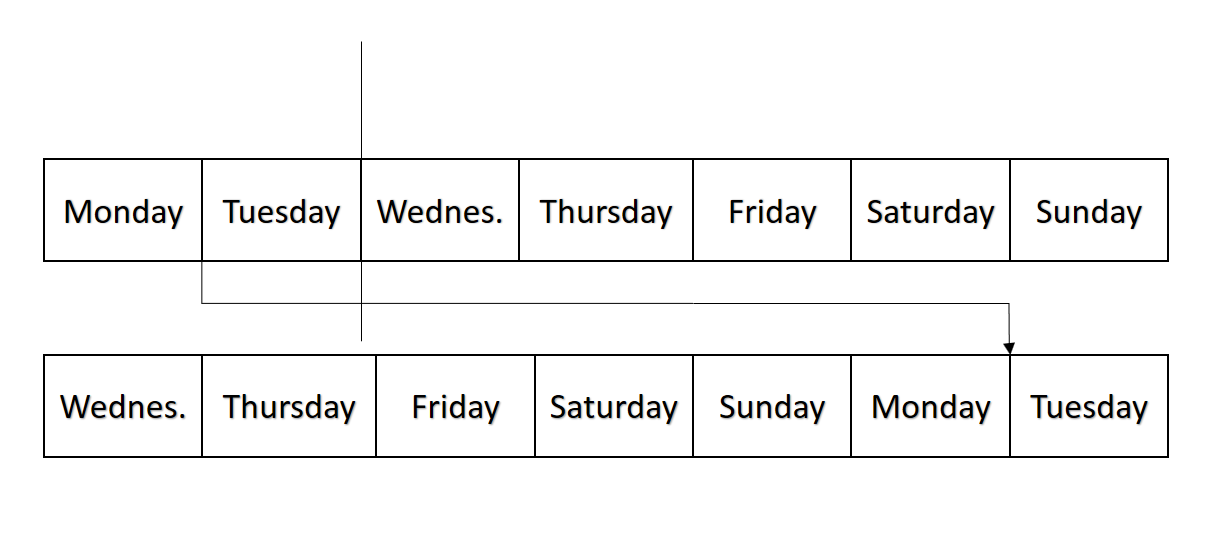
\includegraphics[scale = 0.3]{Images/sportsorting.png}
\caption{Sorting day operation}
\end{figure}
The list of sport types (that the user can select in the combo box) is created in the controller. This one automatically updates and displays sports in alphabetical order. Then the controller communicates all the sport time slots and the list of distinct sports to the HTML that is seen by the user. 
\subsection{Tools}
The only functionality in the tools section is the maps \footnote{\url{https://github.com/mathieuzen/llnmaps}} . We created the menu in order to introduce new functionalities later. 
\subsubsection{LLN Maps}
\paragraph{Design}
LLNMaps has its own header and footer, after a discussion with our contributors about the way to merge them to our application. First, they have a search side menu so we decided to overwrite our settings side menu that is unreachable from the maps. Therefore, the settings button in the header is replaced by a search button. In their footer, they have a compass or map mode. There are several alternatives regarding the footer.
\begin{itemize}
\item Put the compass button in the header
\item Add it in our footer
\item Create a sub footer
\item Create a sub header
\item Put it on the map page (not in a footer or header) 
\end{itemize}
\subsection{City}
For the city section, we only created the menu in order to add new functionalities later. However, this section is more sensitive than other because it add external businesses in the application, so more advanced discussion should take place when adding a functionality.
\subsection{Others}
\subsubsection{Settings menu}
The settings menu can be opened everywhere in the application except for the map.
\paragraph{Design}
This menu is a side menu, which means when the user opens it, it does not take all the screen as a new page. Instead it cuts the screen in two parts. The part on the left is the page where the user opened the settings menu, the second part is the settings menu. That allows the user to change a setting without being disturbed in his current task.
The settings menu offers three items:
\begin{itemize}
\item The language
\item The campus
\item Logout
\end{itemize}
\paragraph{Language} We introduced three different languages, French, Dutch and English. The student can select one of this three languages and all the application will directly been translated into it. The translation in Dutch is not done yet although it is implemented and just needs the actual translations. \\
For the implementation, we used a plugin called "angular-translate" \footnote{\url{https://github.com/angular-translate/angular-translate}}(MIT). This plugin allows to create a configuration where you define the application languages, and for each languages it holds a kind of dictionary with the variables and their translations.\\
Here is an example of the code for translation:
\begin{verbatim}
        $translateProvider.translations('en', {
            hello_message: "Hello",
            goodbye_message: "Goodbye"
        });
\end{verbatim}
In this example, we create an English translation and the variable "hello\_message" is translated by "Hello" in the user interface (same for goodbye). Our application has more variables to translate but the process is exactly the same. One more step is needed to translate the variable, at each time we want a variable in the HTML to be translated we need to apply a translation filter onto it. For example 
\begin{verbatim}
		<html tag>{{"hello_message" | translate}}</html tag> 
\end{verbatim}
The plugin allows to set a preferred language that will be preselected at the application launch. Currently it is English.
\paragraph{Campus selection} The user can select a campus with the button named "Choose my campus" in the settings menu. This button opens a page with the list of all possible campuses, the user has to choose one and validate his choice. As explained earlier the campus selection influences the available functionalities in application. A pre-selection based on the geolocation happens when the user open UCLCampus and the nearest campus is chosen by default.\\
For the implementation, we created a campus factory that holds a list of campuses. The items of this list have three attributes, the name of the campus, longitude and latitude. In order to select the closest campus, we created a JavaScript function that just returns the campus minimizing the distance between it and the current position of the user. Thus it is easy to add a new campus to the application or remove one.
\section{Modularity and how to add a new functionality}
This application was built with the idea that other contributors would have to add functionalities themselves or even take over the project in the future. It was therefore important to be able to add modules to the application without having to understand the whole code. 
This section will present a user manual on how to get the application to run from scratch and how to add new functionalities.  It must be noted that in order to deploy the application on iOS, one must user OS X as his operating system.  The following steps will however work for any operating system and the user will be able to deploy the application on Android regardless of the OS used.
\subsection{Setting up the framework}
\subsubsection{Step 1: Installing Git}
First,  we need to install Git.\\
\textbf{For Windows users}: \\
Go to https://git-scm.com/download/win, download and install Git for Windows. Any further commands in this guide can be executed in either the Git Bash. 
\textbf{For Linux users}: \\
Type the following line of code into your terminal:
\begin{lstlisting}[language=bash]
  $ sudo apt-get install git
\end{lstlisting}


\subsubsection{Step 2: Installing Node.js}

Node.js is a JavaScript runtime that is required to install the other things one needs to install the application. This step slightly differs depending on your OS.\\

\textbf{For Windows users}: \\
Windows users can download an installer from the Node.js website: https://nodejs.org/en/ .\\

\textbf{For Linux users}: \\
First, install Node.js by typing the following command line in your terminal:
\begin{lstlisting}[language=bash]
  $ sudo apt-get install nodejs
\end{lstlisting}
Then, install npm:
\begin{lstlisting}[language=bash]
  $ sudo apt-get install npm
\end{lstlisting}
Finally, create a symbolic link for node:
\begin{lstlisting}[language=bash]
  $ sudo ln -s /usr/bin/nodejs /usr/bin/node
\end{lstlisting}
You can now test that the installation worked properly by running these two commands:
\begin{lstlisting}[language=bash]
  $ node -v
  v0.10.25
  $ npm -v
  1.3.10
\end{lstlisting}
\subsubsection{Step 3: Installing Ionic and its dependencies}
If you are on Windows, drop sudo from the following commands.
\\First, install Cordova:
\begin{lstlisting}[language=bash]
   $ sudo npm install -g cordova
\end{lstlisting}
Then, install Ionic:
\begin{lstlisting}[language=bash]
   $ sudo npm install -g ionic
\end{lstlisting}
\subsection{Installing UCLCampus}
Now that you've set everything up, it's time to fetch the source code of the application from GitHub. 
\subsubsection{Step 1: Forking the project}
First, navigate to https://github.com/amoyaux/UCLCampus. Click the Fork button in the top right corner. Note that in order to fork the project, you will need a GitHub account.
Once you have forked the project, open a terminal into the repository of your choice. Then, enter the following command:
\begin{lstlisting}[language=bash]
   $ git clone https://github.com/<your username>/UCLCampus.git
\end{lstlisting}

This will clone the project files into the chosen repository.

\subsubsection{Step 2: Installing the required packages}

Now you will need to install some packages before running the application. To do so, move to the right directory:

\begin{lstlisting}[language=bash]
   $ cd UCLCampus/UCLCampus/
\end{lstlisting}
Then run the following commands. These commands, except for the first one, can be found in the plugin.txt file.
\begin{lstlisting}[language=bash]
   $ npm install
   $ cordova plugin add cordova-plugin-device
   $ cordova plugin add cordova-plugin-console
   $ cordova plugin add cordova-plugin-whitelist
   $ cordova plugin add org.apache.cordova.network-information
   $ cordova plugin add https://github.com/brodysoft/Cordova-SQLitePlugin.git
   $ cordova plugin add https://github.com/litehelpers/Cordova-sqlite-storage.git
   $ cordova plugin add https://github.com/EddyVerbruggen/Calendar-PhoneGap-Plugin.git
   $ cordova plugin add https://git-wip-us.apache.org/repos/asf/cordova-plugin-inappbrowser.git
   $ cordova plugin add cordova-plugin-geolocation
   $ cordova plugin add https://github.com/brodysoft/Cordova-SQLitePlugin.git
   $ cordova plugin add https://github.com/an-rahulpandey/cordova-plugin-dbcopy.git
   $ cordova plugin add cordova-plugin-network-information
\end{lstlisting}

\subsection{Running the application}

There are several ways to run the application now that it is installed. Note that in order to run it on emulators, you will need to install said emulators and their required dependencies (programming languages, ...). This aspect is not covered in this guide.

\subsubsection{Running the application in an Internet browser}

Since Ionic is an hybrid framework, the application can easily be run in a browser. Simply open a terminal in the UCLCampus/UCLCampus/ folder and run the following command:

\begin{lstlisting}[language=bash]
   $ ionic serve
\end{lstlisting} 
The application is now running on http://localhost:8100/ . However, some functionalities may not work properly, namely the ones that need access to the SQLite database. This is due to the fact that opening the database is not done in the same way for a browser or a mobile device. It would be possible to add support for the database in this case, but this was not a priority as the focus of the application is not to be run in a browser.
\subsection{Running the application on a device or emulator}
Once you have installed the emulator or connected the device to your computer, you need to add the corresponding platform to Ionic using the following command:
\begin{lstlisting}[language=bash]
   $ ionic platform add android
\end{lstlisting} 

or

\begin{lstlisting}[language=bash]
   $ ionic platform add ios
\end{lstlisting} 
Note that to run the application on an IOS device, you will need a Mac computer. Now that the device is connected and the platform is added, simply run the following the run the application:
\begin{lstlisting}[language=bash]
   $ ionic run android
\end{lstlisting} 

or 

\begin{lstlisting}[language=bash]
   $ ionic run ios
\end{lstlisting} 
For more options on the launch command, please refer to http://ionicframework.com/docs/cli/run.html.
\subsection{Adding a new functionality}
Now that everything is up and running, new functionalities can be added. This guide will explain how to add a new functionality to the Tools section. The same steps can be repeated to add new functionalities to any section of the application.
\subsubsection{Step 1: Creating the required files}
First, you will need to create the required files for your functionality. Navigate to the UCLCampus/UCLCampus/www folder. In this folder, we can see the architecture of the project. It contains one folder for each section of the application. Now, since we want to add a functionality to the Tools section, navigate to the tools folder. Here you can see 3 folders: ''js'', ''templates'' and ''maps''. ''js'' and ''templates'' are the folders that handle the tools menu in the application while ''maps'' is a functionality. So to create a new functionality, you will need to create a new folder.
Create a new folder named ''my\_functionality''. Now navigate to this folder and create two new folders, ''js'' and ''templates''. ''js'' will contain your JavaScript while templates will contain your html code. In the ''js'' folder, create a ''my\_functionality.js'' file and create a ''my\_functionality.html'' file in the ''templates'' folder.
\subsubsection{Step 2: Writing the JavaScript code}
Open your favorite text editor and open the ''my\_functionality.js'' file. In this file, paste the following code:
\begin{lstlisting}[language=JavaScript]
   angular.module('ionicApp').controller("MyFunctionalityController", function($scope) {
      $scope.textToDisplay = "This is the text we want to display."
   });
\end{lstlisting} 
\subsubsection{Step 3: Writing the HTML code}
Open the ''my\_functionality.html'' file.   In this file, paste the following code:
\begin{lstlisting}[language=HTML]
   <ion-view title="Title">
      <ion-content>
         <div>
            {textToDisplay}
         </div>
      </ion-content>
   </ion-view>	
\end{lstlisting} 
\subsubsection{Step 4: Adding your functionality to the application}
To add the functionality to the application you will first need to create a state for it. To do so, open the UCLCampus/UCLCampus/www/js/app.js file. In this file, you will find the state provider. It contains a list of all the states the application can be in. You need to add a state for your functionality. Find this state in the list:
\begin{lstlisting}[language=JavaScript]
.state('app.tools', {
    url: "/tools",
    cache : false,
    views: {
      'tools-tab' :{
        templateUrl: "tools/templates/tools.html",
        controller: "ToolsController"
      }
    }
  })
\end{lstlisting} 
This state corresponds to the tools menu. Below this state, add the following new state:
\begin{lstlisting}[language=JavaScript]
.state('app.myfunctionality', {
    url: "/myfunctionality",
    views: {
      'tools-tab' :{
        templateUrl: "tools/my\_functionality/templates/my\_functionality.html",
        controller: "MyFunctionalityController"
      }
    }
  })
\end{lstlisting} 
Once this is done, open the UCLCampus/UCLCampus/www/index.html file. In this file, find the following lines:
\begin{lstlisting}[language=HTML]
   <!-- tools module -->
   <script src="tools/js/tools.js"></script>
\end{lstlisting}
Below these lines, add the following:
\begin{lstlisting}[language=HTML]
   <script src="tools/my_functionality/js/my_functionality.js"></script>
\end{lstlisting}
Your functionality has now been added to the application ! However, we don't have a way to access it yet. We will therefore add a button in the tools menu to access it. Open the UCLCampus/UCLCampus/www/js/factory.js file. This file handles, among other things, the buttons we can see in the different menus of the application. Find the function called "ToolsMenuFactory".  In this function you can see the following code:
\begin{lstlisting}[language=JavaScript]
   toolsMenuList : [
       { title: 'Maps' , icon:'icon ion-map royal', url:'app.maps', campus:['Louvain-la-Neuve']}
   ], 
\end{lstlisting}
Change it to the following:
\begin{lstlisting}[language=JavaScript]
   toolsMenuList : [
      { title: 'Maps' , icon:'icon ion-map royal', url:'app.maps', campus:['Louvain-la-Neuve']},
      { title: 'My functionality' , icon:'icon ion-help royal', url:'app.myfunctionality', campus:[]}
    ],
\end{lstlisting}
The campus field in each item is used if you want to create functionalities specific to one or several, but not all, campuses. For instance, the maps functionality is currently only available for the Louvain-La-Neuve campus. An empty campus field means that we can access the function from all campuses.
You can now access the new functionality from the tools menu of the application. You can now start editing the JavaScript and HTML files to create a more complicated function.
\subsubsection{Step 5: submitting your functionality}
Once you have completed a functionality and believe it is ready to be integrated into the application, you can send a pull request to the project owner. The pull request will then be reviewed and will be added to the application if it is accepted. For more information about forks and pull requests, please refer to: https://help.github.com/articles/using-pull-requests/ and https://help.github.com/articles/fork-a-repo/.
\section{Future functionalities and possible improvements}
In this section, we will review the functionalities we couldn't add to the current application for various reasons, as well as looking at ways we could improve the existing functionalities.
\subsection{Future functionalities}
\subsubsection{The "City" module}
In chapter 3, we described the "City" module where a user could find information about museums, cinemas, restaurants and so on. This module was not implemented yet for different reasons. The challenging part about such a module is that some restaurants might not want to be listed in the application. Another challenge is the lack of any database concerning the restaurants of a given campus. It would therefore be necessary to list all restaurants, museums and other activity centers of all campuses and possibly ask them whether they want to appear in the application or not.
While this module would certainly be interesting for the user, it would also be hard to keep the information up to date without having someone responsible to update the application every year or so.
\subsubsection{"Cercles" and "Kot à Projets"}
The "Cercles" and "Kot à projets" functionalities were also supposed to be implemented but weren't for reasons similar to the city module. It would also be necessary to list them and ask them if they want to be listed in the application, as well as maintaining the database up to date since "Kot à Projets" change almost every year.
\subsubsection{Integrating OSIS}
At the time  of writing the UCL was changing its infrastructure. Integrating OSIS, the new architecture, into the application was scheduled but sadly couldn't be achieved. OSIS was going to be used to fetch the courses a student is enrolled in at a given time and displaying information about said courses. 
For now the information is given by a dummy server and doesn't correspond to the reality. An interesting thing to do would therefore be to integrate OSIS to the application as soon as possible.  It is indeed our belief that this functionality is of paramount importance if we want the application to be successful. 
\subsubsection{Tools}
The "Tools" module currently only contains the "Maps" functionality. Other functionalities could be added to this module, such as a functionality regarding how to reach a campus using common transportation, or how to park in the city.
\subsection{Possible improvements of existing functionalities}
\subsubsection{Adding support for all campuses}
A lot of functionalities are only supported by a few campuses so far. We list here the functionalities that would benefit from being supported by multiple campuses:
\begin{itemize}
\item Lecture halls
\item Libraries
\item Events
\item Sports
\item Cafeterias
\item Cercles
\item Kot à projets
\item The entire "City" module
\item Maps
\end{itemize}
\subsection{Other improvements}
\begin{itemize}
\item This project currently uses the 1.3 version of Ionic. It is however already possible to use Ionic 2 and migrating the application to this new version could be interesting. At the time of writing Ionic 2 was only available as a beta release, which is why we didn't use it immediately. Ionic 2.0 is interesting because it deploy tools for the tree architecture that is used (see chapter 4.1).
\item Another improvement is to create a logo and a splash screen for the application.
\item Finish the Dutch translation. Everything is implemented, the only thing that is missing the map between the variables and their translations.
\item Support the functionalities that use the database on browsers. 
\end{itemize}
\section{Tests}
There are two different kinds of tests. The first kind is unit tests, these tests are simple and ensure that a factory or a function returns the correct result. It can also test the local and global page variables. These tests are designed to test one functionality at a time.
The second tests are the end to end tests. These tests represent a real world scenario. It allows to test a sequence of functionalities and dependencies between them.
\subsection{Unit Tests}
There are two type of unit tests. The first aims at controlling a factory response. The second analyses the controllers variables.
\subsubsection{Step 1: Installing the test}
Installing some packages is needed to before running the tests. To do so, move to the appropriate directory:
\begin{lstlisting}[language=bash]
   $ cd UCLCampus/UCLCampus/
\end{lstlisting}

Then, install the dependencies by running the following commands in terminal\footnote{If it fails, try to run npm commands with sudo}
\begin{lstlisting}[language=bash]
   $ npm install karma karma-jasmine karma-phantomjs-launcher --save-dev
   $ npm install -g karma-cli
   $ bower install angular-mocks --save-dev
\end{lstlisting}
At this step, it would be needed to create a configuration file but we have already did it. This file is in the tests directory and is named \textit{my.conf.js}. Open it and add your JavaScript and tests in the files object.
\subsubsection{Step 2: Running the tests} 
To run the tests, use the following command.
\begin{lstlisting}[language=bash]
   $ karma start tests/my.conf.js
\end{lstlisting}
It is not needed to run this command after each modification. These tests run in the background and are automatically recalculated after a change. Figure 5.3 shows the result.
\begin{figure}[H]
\centering
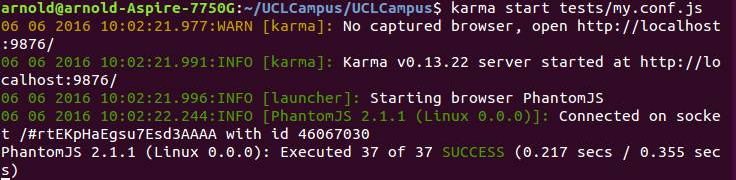
\includegraphics[scale = 0.7]{Images/tests.png}
\caption{Test results}
\end{figure}

\subsubsection{Current Tests}
There are two folders, one for controller tests and the other for factory tests. The current set of tests ensures that factories return the good result. There is not a lot of tests on controllers because the majority of variables come from factory results. There is actually a important restriction. The test are made on a browser and some functionalities don't work on it. This implies that some functionalities couldn't be tested such as \textit{Lecture Halls} and\textit{ Libraries }for example. Indeed, these functionalities cannot be run through a browser and require either a smartphone or an emulator to work properly. 

\subsection{End to End Tests}

End to End tests open a browser and carry out actions just like a real person. These tests allow to test dependencies among functionalities. For example login with specific credentials, accessing the schedule page, test if the schedule class slots are consistent with the credentials. Another example is to test the interface change after a campus site modification.

\subsubsection{Step 1: Installing the tests}

First go to the main repository
\begin{lstlisting}[language=bash]
   $ cd UCLCampus/UCLCampus
\end{lstlisting}
Then, install the dependencies\footnote{If webdriver-manager update fails, pass in root mode 'sudo -s' and try again}.
\begin{lstlisting}[language=bash]
   $ npm install -g protractor
   $ webdriver-manager update
\end{lstlisting}
We already created the configuration file. It is named\textit{ e2e-tests.conf.js} if you want to modify it. It is currently configured to run the tests on chrome.
\subsubsection{Step 2: Running the tests}
First run the application on localHost.
\begin{lstlisting}[language=bash]
   $ ionic serve --nobrowser
\end{lstlisting}

Then run the tests.

\begin{lstlisting}[language=bash]
   protractor tests/e2e-tests.conf.js
\end{lstlisting}

It will run the tests on the browser with a visual feedback and return a more detailed feedback in terminal as shown in figure 5.4.

\begin{figure}[H]
\centering
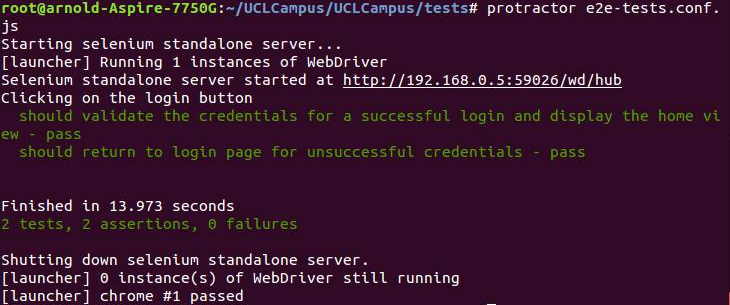
\includegraphics[scale = 0.7]{Images/test2.png}
\caption{End to End Tests results}
\end{figure}


\subsubsection{Our tests}
We tested the login functionality with correct and incorrect credentials.
Currently there are no other tests but it would be interesting to test the schedule and the change after a new campus selected.\\
Again, all the tests are in browser, and functionalities that work with device functions could not be tested. 
\chapter{Analysis}

Once the application was implemented, we needed to reflect on the choices we made along the way and try to determine whether they were the right ones or not. We also analyze the application as a whole. The first section gives some quantitative data regarding the source code of the application while the second section explains some tests we made to determine the performances of our finished product. Finally, the last section gives some insight on hybrid approaches and more specifically the Ionic framework.

\section{Quantitative analysis}

This section will give some quantitative data regarding the application's source code. This data can be used to get an idea of the amount of work needed to implement a similar application.

\subsection{Lines of code and files}

GitHub lists the total number of lines of the whole project as a staggering 397,656. This number by itself does not mean much as it includes generated binary files and other computer generated files. We will therefore look at the code actually written by hand. This code is divided in three languages, namely JavaScript, HTML and CSS. In this code, there is the code that was written by the authors of this thesis as well as the code written by other contributors. Aside from this code is the SQL code we wrote to update the database with various details. This code is however not documented and is therefore not listed here.

\subsubsection{JavaScript code}

\begin{itemize}
\item Number of JavaScript files written by the authors: 16
\item Number of lines of code written in JavaScript by the authors: 1696
\item Number of JavaScript files written by other contributors: 12
\item Number of lines of code written in JavaScript by other contributors: 602
\end{itemize}

\subsubsection{HTML code}

\begin{itemize}
\item Number of HTML files written by the authors: 16
\item Number of lines of code written in HTML by the authors: 2942
\item Number of HTML files written by other contributors: 2
\item Number of lines of code written in HTML by other contributors: 57
\end{itemize}

\subsubsection{CSS code}

\begin{itemize}
\item Number of CSS files written by the authors: 1
\item Number of lines of code written in CSS by the authors: 309
\item Number of CSS files written by other contributors: 2
\item Number of lines of code written in CSS by other contributors: 880
\end{itemize}

\section{Performance testing}

In order to assess the performance of our application, we profiled it using Google Chrome. Google Chrome indeed has a tool, available using the chrome://inspect address, that allows developers to profile an application running on their Android device. The following results are therefore only relevant for Android phones. The device we used for these tests was a Huawei P8 Lite, a smartphone with average performances (source benchmark). Results may vary with higher or lower end smartphones. Despite the limitations of our testing, the results are still interesting and we will present them in this section.
\subsubsection{Profiling}
We used Google Chrome tool in order to profile several functionalities of our application. It is important to note that monitoring and recording the application's activity adds a bit of overhead and the results we show here will be slightly worse than the ones one would obtain without any monitoring tool. However, the overhead is not important enough to invalidate the results. The idea is to start the profiling, click a button and wait until the next view is displayed. This gives us an idea of how long a user has to wait between views. Figure 6.1 shows the result we obtained when clicking on the "Libraries" button in the Student Menu. The rest the profiles are available in annex X (TODO).\\

\begin{figure}
\centering
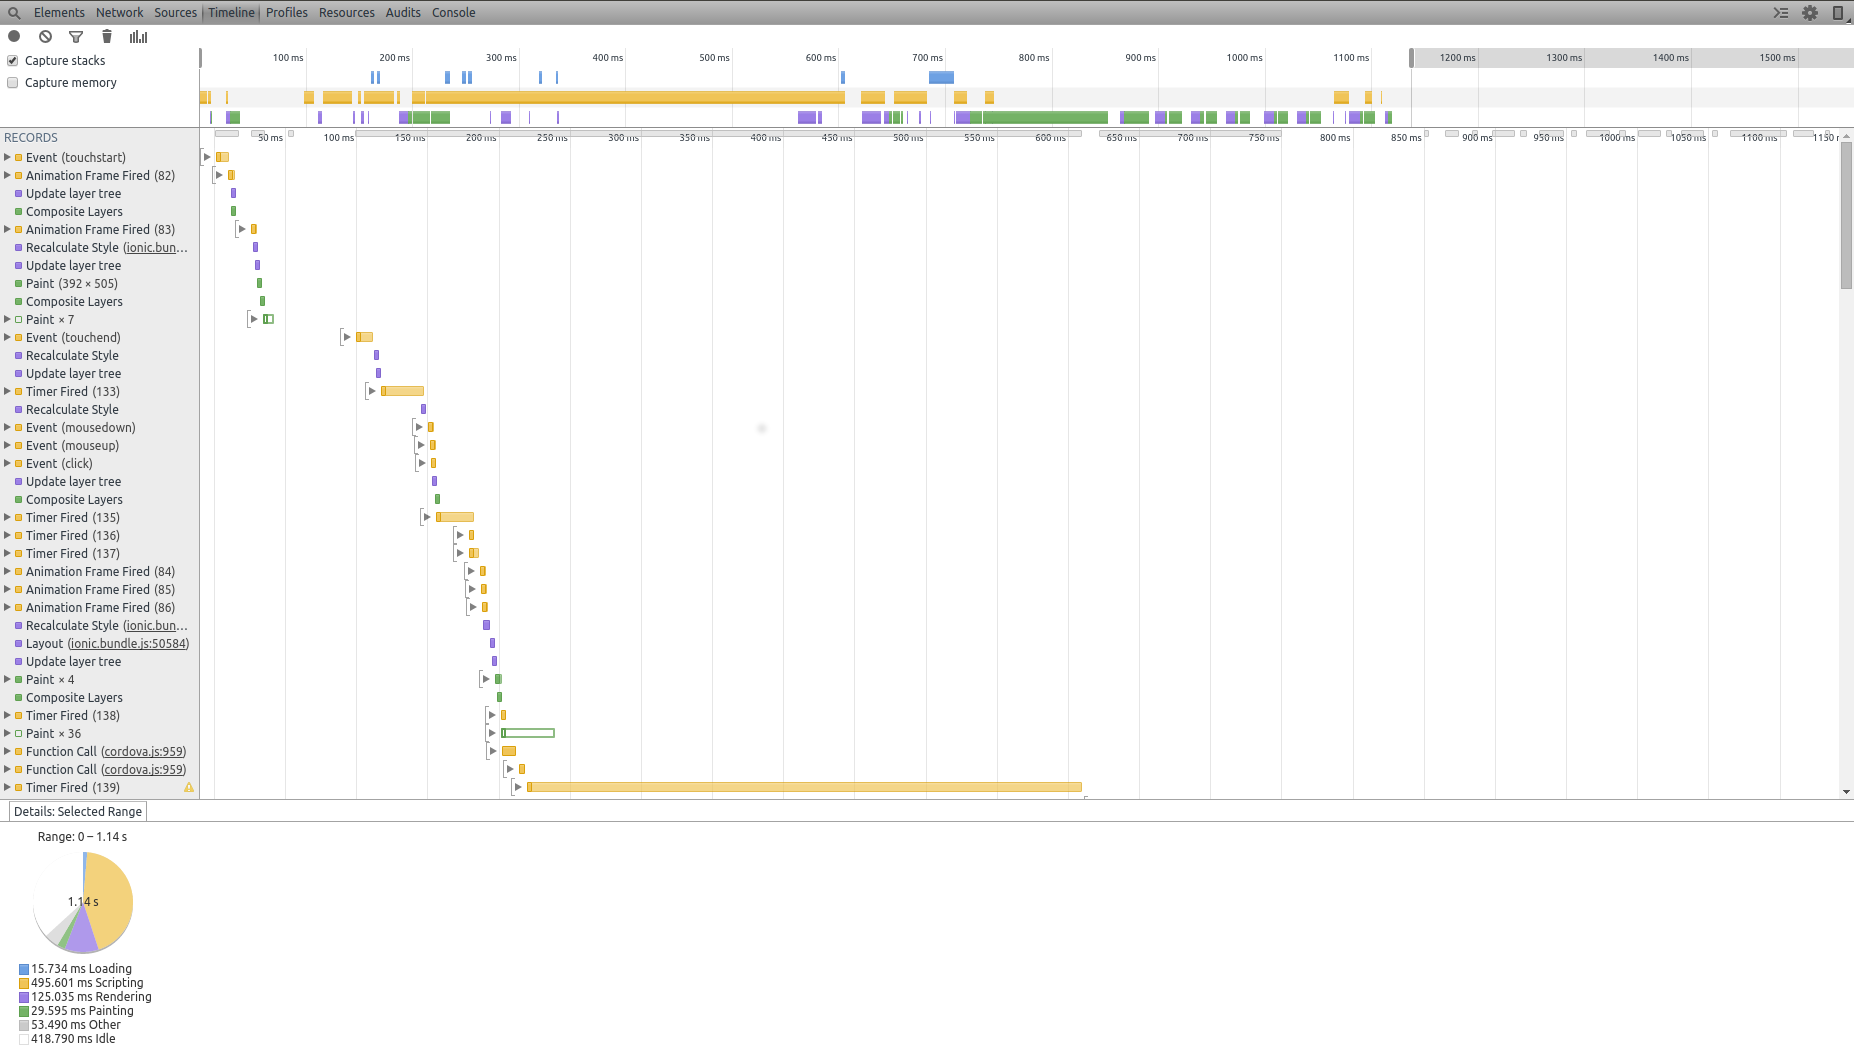
\includegraphics[scale = 0.25]{Images/libraries.png}
\caption{Profile of the Libraries functionality}
\end{figure}

In this figure we can see several interesting things. We start by observing that the application takes approximately 1.1 seconds to display the list of libraries. We ignore the last 0.04 seconds displayed in the figure as the work was done and the rest of the time was spent idle. The rest is split among several tasks:
\begin{itemize}
\item Scripting : Running the JavaScript code. Time spent: 495.601ms, 45\% of total time
\item Loading : Loading different resources (images, ...) from memory. Time spent: 15.734ms, 1.4\% of total time
\item Rendering : Organizing the page layout. Time spent : 125.035ms, 11.4\% of total time
\item Painting : Displaying the view. Time spent : 29.595ms , 2.7\% of total time
\item Other. Time spent : 53.49ms, 4.9\% of total time
\item Idle. Time spent : 385ms, 35\% of total time
\end{itemize}
We can see that, despite displaying several images, the application only spends 14.1\% of its time to render and paint said images. Instead, most of the time is spent scripting. This means that the most time consuming thing the application does when displaying the libraries is finding said libraries in the database and converting the result to a JavaScript list. This behavior seems to remain the same for every functionality of the application. Indeed, scripting is usually the main task in every profile, ranging anywhere from 30 to 60\% of the total execution time. 
We will now look at the execution times of other functionalities: 
\begin{itemize}
\item Changing tabs : 489ms
\item Displaying the schedule : 2005ms
\item Displaying the list of sports : 4260ms
\item Displaying the student menu : 700ms
\item Displaying the Cafeterias : 1051ms
\item Displaying the campus menu : 970ms
\item Displaying the events : 2890ms
\item Displaying the details of an item (library, lecture hall, ...): ~700ms
\item Displaying the list of lecture halls: 1290ms
\item Displaying the map: 3650ms
\end{itemize}  
From these results, we can observe 3 types of functionalities:
\begin{itemize}
\item Simple display of information already available. Takes less than a second. Examples: changing tabs, loading a menu, displaying details of an item.
\item Display of information available in the local database. Takes between one and two seconds.
\item Display of information available online and maps. Takes more than two seconds.
\end{itemize}
These results make a lot of sense since retrieving information online means we have to wait for the server to respond, which explains the overhead. There is not much we can do to avoid waiting for the server aside from caching the results in the application. Caching the results is also possible for functionalities retrieving information from the database. This technique significantly increases performances but only does so after the user already used the functionality a first time. We observe the following performances once the results have been cached:
\begin{itemize}
\item Displaying the list of lecture halls: 834ms
\item Displaying the list of libraries: 782ms
\item Displaying the Cafeterias: 754ms
\item Displaying the schedule: 1530ms

\item Displaying the list of sports: 1350ms
\end{itemize}
We can observe a significant performance increase once the results have been cached in these functionalities, usually around 500ms and almost 3 seconds for the list of sports. This is due to the slow response time of the server we contact to retrieve the sports. The other slower functionalities (maps and events) cannot be easily cached. Indeed, it does not make sense for maps as there are no results to be cached. As for the events, the list is constantly updated and caching the result might lead to inaccurate information being displayed.
We can now see that, once the relevant information has been cached, most functionalities respond in less than a second. We could not find any standard regarding the recommended response time for an application. However, Android will consider the application as not responding if it stuck for more than 5 seconds. As we can see, none of our functionalities exceed this limit, even when not cached.\\

The response time ranging between 500 and 1000 ms is considered to be immediate\footnote{\url{https://www.smashingmagazine.com/2015/09/why-performance-matters-the-perception-of-time/}}, which is the recommended interval to load pages. Most of our functionalities are in this range. In order to make the wait for slower functionalities more bearable, we added an indicator that the functionality is loading. That way the user still receives feedback to indicate that his action, in this case the press of a button, has been registered and that the application is working on it. \\

We conclude that, despite using a hybrid framework, the performances of our application are acceptable and that most users will not notice any delay when using the majority of the functionalities. Furthermore, the slowest functionalities often depend on the response times of external servers.. In those cases, using a native approach would not have helped performance-wise. 

\section{Ionic Framework}
Working on UCLCampus allowed us to experience the Ionic Framework. We learned that it had some benefits and some downsides we will now expose.

\subsection{Benefits}
\begin{itemize}
\item Easy to learn and use. The tutorial on their website is complete and brings possible architecture notions. This tutorial, combined with a tutorial about AngularJS \footnote{We used the w3school tutorials available at \url{http://www.w3schools.com/angular/}}, makes it possible to start an application right away. 
\item The CSS and JavaScript code provided are useful and well designed. Around 90\% of the css components and icons used come from it.
\item A large community that provide quick response and many examples for simple topics. Moreover, this community provides a great panel of plugins, meaning it was never necessary to create our own. 
\item Well documented. Every component is listed and described and some basic examples are provided.
\item AngularJs provides a rich architecture to modulate the source code. 
\item Easy to handle web services and database management. 
\item Very decent performances. See section 6.2.1 for details.
\item The application does not feel emulated.
\end{itemize}

We can see that the Ionic Framework held its initial promises. The application has a good native look and feel and for the most part, the documentation and community were great. We however encountered some minor issues for which we were unable to find any solutions. 

\subsection{Drawbacks}
\begin{itemize}

\item No response for advanced topics. 
\item Bug report still has not been answered 3 months after the report. 
\item A poor architecture for HTTP requests to external website. 
\item Some plugins and components still in development and contain some bug.
\item Some functionalities and factories need a specific code for browser. 

\end{itemize}

We encountered a minor bug in our application. Indeed, when changing the Category filter in the events functionality, the new filter will be applied but the display of the selection tool will not be updated the first time it is used. Every subsequent attempt updates the view just fine. We reported this bug on the Ionic project GitHub but sadly never received an answer. We admit that the bug is minor and that the Ionic team probably has more important issues to tackle but we still were disappointed to receive no answer.\\

Another issue we encountered was when we tried to use cookies in external websites requests. Ionic removed "cookie" and "set-cookie" in the response parameters. That is a real problem when a website uses a cookie authentication or parameters inside the cookie. The reason is that they implemented a local cookie storage which is more efficient. However, it only works for request inside the application.
We could not find a way to work around this problem.\\

Finally, some of the plugins we found contained some bugs, for instance the calendar plugin.\\

As we can see Ionic is not perfect but the issues we encountered were minor and the overall experience is still overwhelmingly good. We therefore recommend it to people wishing to start their own application and to the future students working on UCLCampus.

\chapter{Conclusion} 

This thesis exposed the whole development process we followed in order to develop the UCLCampus application, starting with an analysis of the existing tools, followed by the implementation itself and finishing with an analysis of the project once it was done.\\

Aside from analyzing the finished application itself, we also need to reflect on the thesis as a whole, especially regarding the two contributions we described in the introduction.\\

The first contribution we wanted to make was to allow other people to use this thesis as a reference to start a new application themselves. While we had trouble finding relevant information regarding the different options we had we still believe that the second chapter of this thesis can be helpful, even though the information found there might soon be irrelevant if the field evolves too much.
We consider chapter 6 to be really useful for the targeted readers as it provides quantitative data regarding performances and remarks concerning one of the most used hybrid framework nowadays.\\

The second contribution we were aiming for was the application and the hope that this application would be continued by other students in the future. We think we have provided a solid basis for future students to work on despite not being able to implement all the functionalities we had in mind. Indeed, one of the many learning outcomes of this thesis was that it is not easy to evaluate the time required to accomplish a task without a deep understanding of the underlying technology you are using. We however do not consider this to be a failure as it was planned from that start that the application would be further developed in the future.\\

Another important learning outcome is the hands-on experience we were able to get through working on a full scale project. We were indeed able to learn languages such as JavaScript, HTML and CSS and familiarize ourselves with Cordova, AngularJS and the Ionic Framework. This knowledge and experience was something that was lacking in our academic background. We furthermore believe that we would not have been able to acquire such useful and highly demanded skills through a more theoretical thesis.\\

This project also helped us develop our communication skills as it was imperative to expose the work that had currently been done both to our supervisor but also to the other contributors. We had to give them regular feedback and clearly expose our ideas as well as take their criticism into account when working on the application.\\

\newpage

We also put other skills that were already present in our academic background to the test, realizing that our existing knowledge was not always enough. Such skills include SQL which we used to access the database but also and more importantly our project management skills. A project of this magnitude indeed requires careful planning and we might have been able to do even more had we planned accordingly.\\

We are nonetheless satisfied with our finished products and hope the students who will take over the project will make it even better. We also hope these students as well as other researchers will put this thesis to good use.\\
\begin{thebibliography}{9}

\bibitem{} 
Andre Charland , Brian Leroux.
\textit{Mobile application development: web vs. native}. 
Communications of the ACM, v.54 n.5, May 2011  

\bibitem{} 
Mario Korf and Eugene Oksman. 2015.
\textit{Native, HTML5, or Hybrid: Understanding Your Mobile Application Development Options}.
[ONLINE] Available at: https://developer.salesforce.com/page/Native,\_HTML5,\_or\_Hybrid:\_Understanding\_Your
\_Mobile\_Application\_Development\_Options. [Accessed 19 May 2016].


\bibitem{} 
Krishnan R Menon. 2015.
\textit{Hybrid vs Native Mobile App. Decide in 5 minutes!}.
[ONLINE] Available at: http://julyrapid.com/hybrid-vs-native-mobile-app-decide-5-minutes/. [Accessed 26 May 2016].
 
\bibitem{}
Jay Raj. 2014. 
\textit{The Top 7 Hybrid Mobile App Frameworks}. 
[ONLINE] Available at: https://www.sitepoint.com/top-7-hybrid-mobile-app-frameworks/. [Accessed 8 December 2015].

\bibitem{}
Sunil Arora. 2016. 
\textit{10 Best Hybrid Mobile App UI Frameworks: HTML5, CSS and JS}. 
[ONLINE] Available at: http://noeticforce.com/best-hybrid-mobile-app-ui-frameworks-html5-js-css. [Accessed 6 December 2015].

\bibitem{} 
Danny Markov. 2015.
\textit{Comparing The Top Frameworks For Building Hybrid Mobile Apps}.
[ONLINE] Available at: http://tutorialzine.com/2015/10/comparing-the-top-frameworks-for-building-hybrid-mobile-apps/. [Accessed 18 May 2016].

\bibitem{} 
Richard Stallman. 2016.
\textit{Why Open Source misses the point of Free Software}.
[ONLINE] Available at: http://www.gnu.org/philosophy/open-source-misses-the-point.html. [Accessed 15 March 2016].

\bibitem{} 
Debian. 2016. 
\textit{License information}.
[ONLINE] Available at: http://www.debian.org/legal/licenses/. [Accessed 16 March 2016].

\bibitem{} 
Black Duck. 2016.
\textit{Top Open Source Licenses}. 
[ONLINE] Available at: https://www.blackducksoftware.com/top-open-source-licenses. [Accessed 25 March 2016].

\bibitem{} 
Brett Smith. 2014.
\textit{A Quick Guide to GPLv3}. 
[ONLINE] Available at: http://www.gnu.org/licenses/quick-guide-gplv3.en.html. [Accessed 13 April 2016].

\bibitem{}
Denys Mishunov. 2015.
\textit{Why Performance Matters, Part 1: The Perception Of Time}. 
[ONLINE] Available at: https://www.smashingmagazine.com/2015/09/why-performance-matters-the-perception-of-time/. [Accessed 10 May 2016].

\newpage

\bibitem{}
Ashteya Biharisingh. 2015. 
\textit{How To Write Automated Tests For Your Ionic App - Part 1}. 
[ONLINE] Available at: http://gonehybrid.com/how-to-write-automated-tests-for-your-ionic-app-part-1/. [Accessed 26 May 2016].


\bibitem{}
Andrew McGivery. 2015.
\textit{Unit Testing Your Ionic Framework App}. 
[ONLINE] Available at: http://mcgivery.com/unit-testing-ionic-app/. [Accessed 27 May 2016].

\bibitem{}
PassMark Android Benchmark. 2016. 
\textit{Android Benchmarks, Performance Comparison of Android Devices}. 
[ONLINE] Available at: http://www.androidbenchmark.net/. [Accessed 12 May 2016].
\end{thebibliography}
\newpage

\appendix
\chapter{InVision Screenshots}


\chapter{UCLCampus Screenshots}
\begin{figure}[H]
    \centering
\begin{subfigure}[b]{0.3\textwidth}
        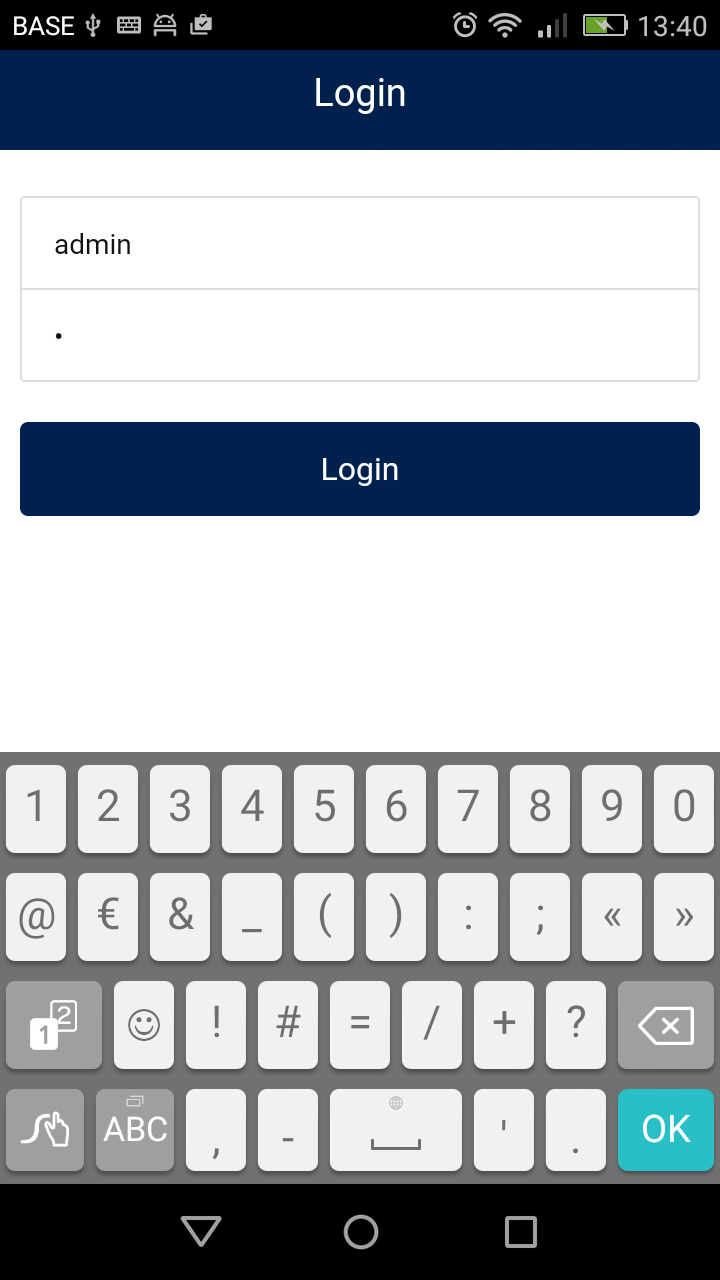
\includegraphics[width=\textwidth]{Images/Application_screens/Screenshot_2016-06-06-13-40-15.png}
    \end{subfigure}
    ~ %add desired spacing between images, e. g. ~, \quad, \qquad, \hfill etc. 
      %(or a blank line to force the subfigure onto a new line)
    \begin{subfigure}[b]{0.3\textwidth}
        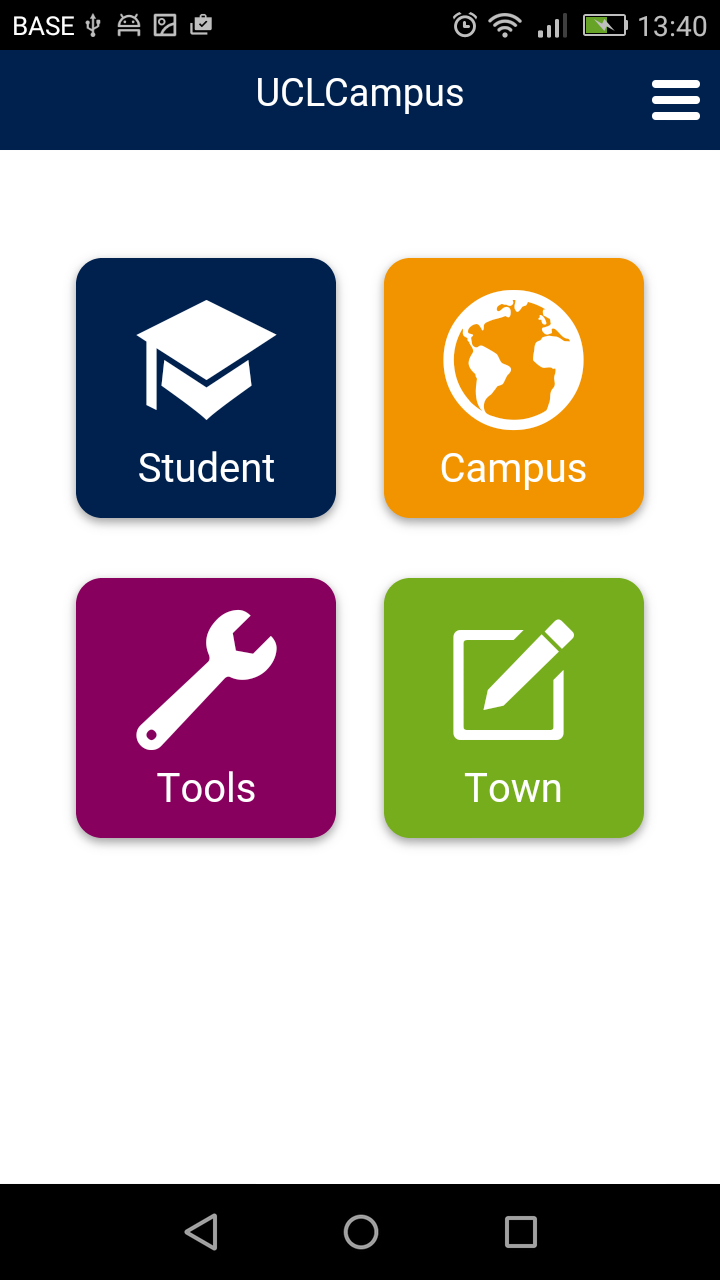
\includegraphics[width=\textwidth]{Images/Application_screens/Screenshot_2016-06-06-13-40-50.png}
    \end{subfigure}
    ~ %add desired spacing between images, e. g. ~, \quad, \qquad, \hfill etc. 
    %(or a blank line to force the subfigure onto a new line)
    \begin{subfigure}[b]{0.3\textwidth}
        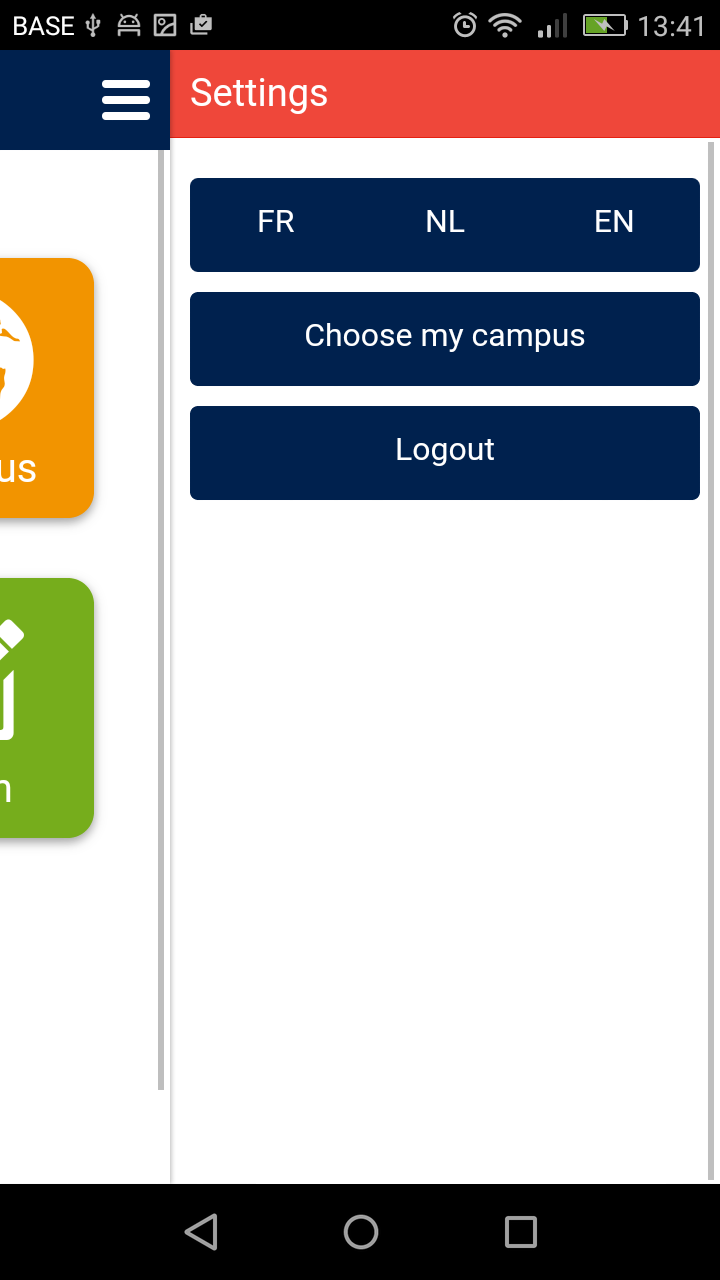
\includegraphics[width=\textwidth]{Images/Application_screens/Screenshot_2016-06-06-13-41-05.png}
    \end{subfigure}
\end{figure}
\begin{figure}
    \centering
\begin{subfigure}[b]{0.3\textwidth}
        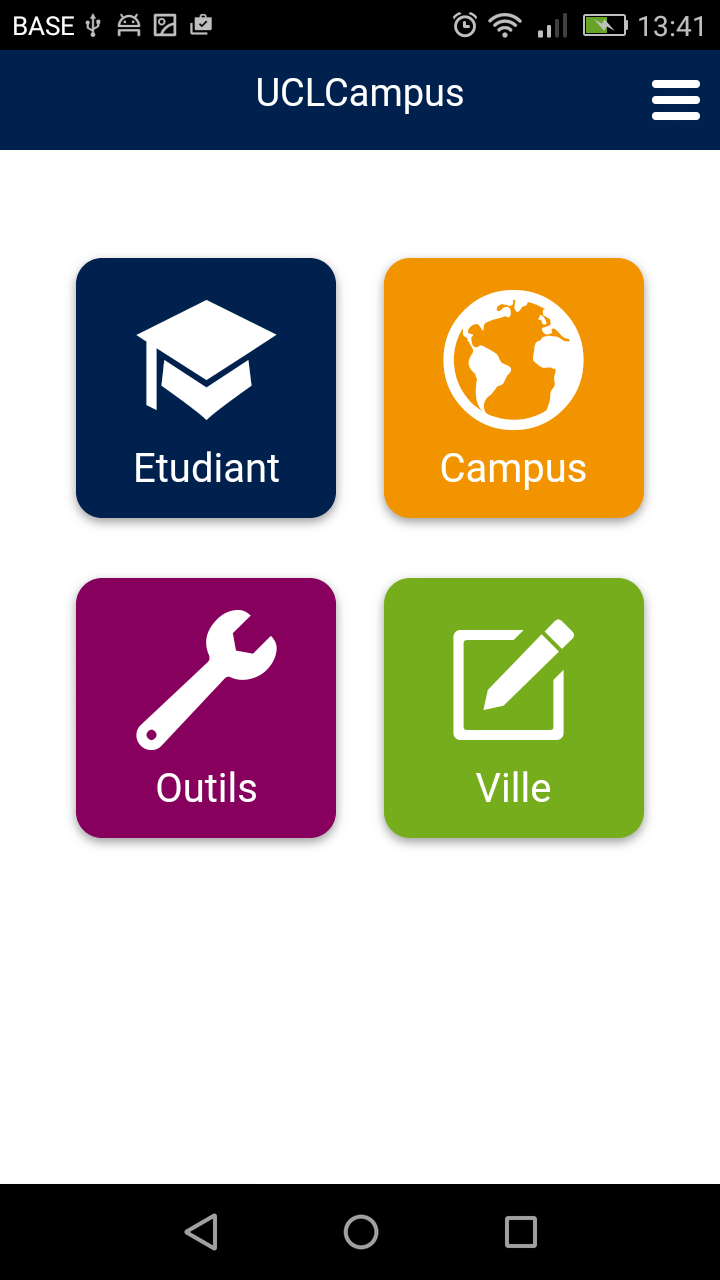
\includegraphics[width=\textwidth]{Images/Application_screens/Screenshot_2016-06-06-13-41-26.png}
    \end{subfigure}
    ~ %add desired spacing between images, e. g. ~, \quad, \qquad, \hfill etc. 
      %(or a blank line to force the subfigure onto a new line)
    \begin{subfigure}[b]{0.3\textwidth}
        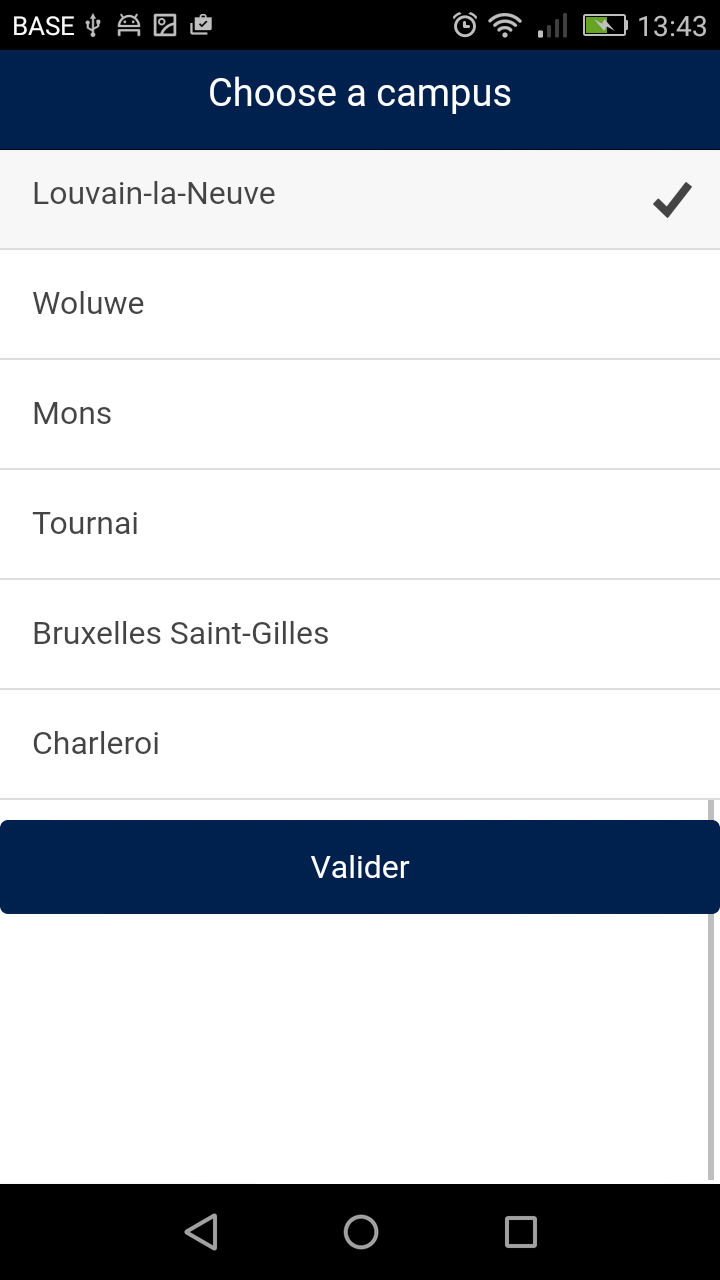
\includegraphics[width=\textwidth]{Images/Application_screens/Screenshot_2016-06-06-13-43-14.png}
    \end{subfigure}
    ~ %add desired spacing between images, e. g. ~, \quad, \qquad, \hfill etc. 
    %(or a blank line to force the subfigure onto a new line)
    \begin{subfigure}[b]{0.3\textwidth}
        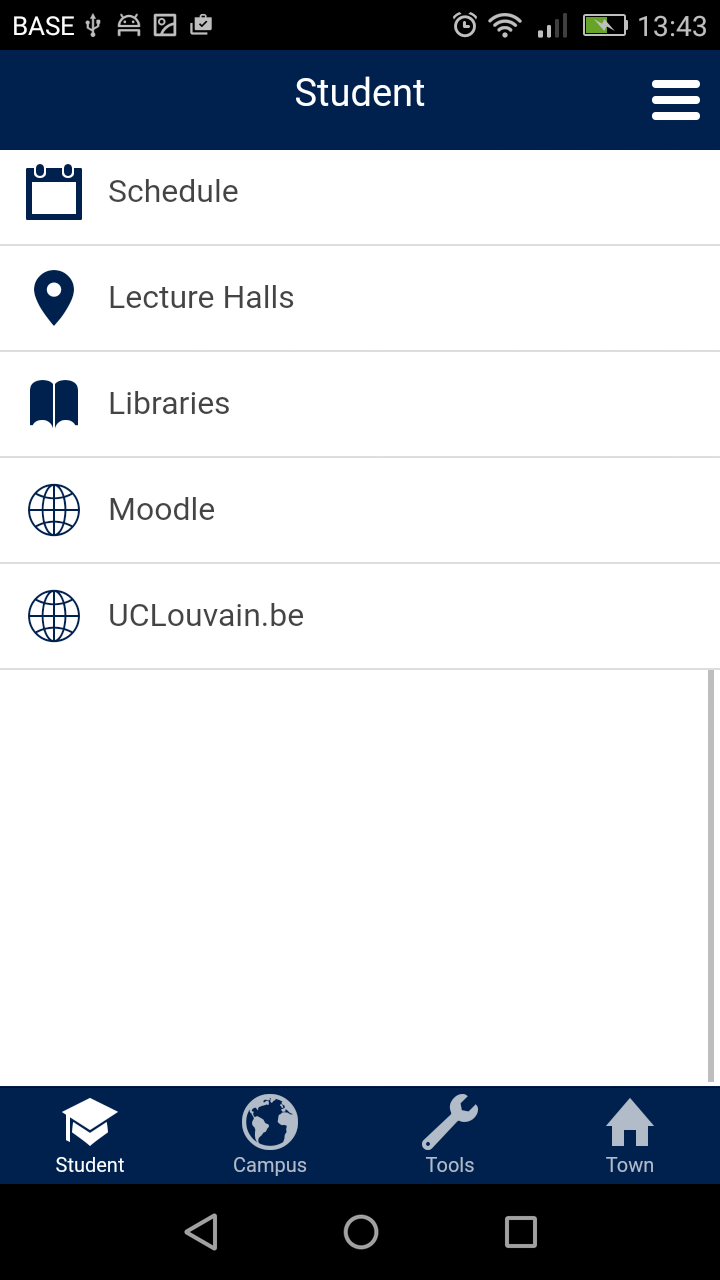
\includegraphics[width=\textwidth]{Images/Application_screens/Screenshot_2016-06-06-13-43-30.png}
    \end{subfigure}
\end{figure}
\begin{figure}
    \centering
\begin{subfigure}[b]{0.3\textwidth}
        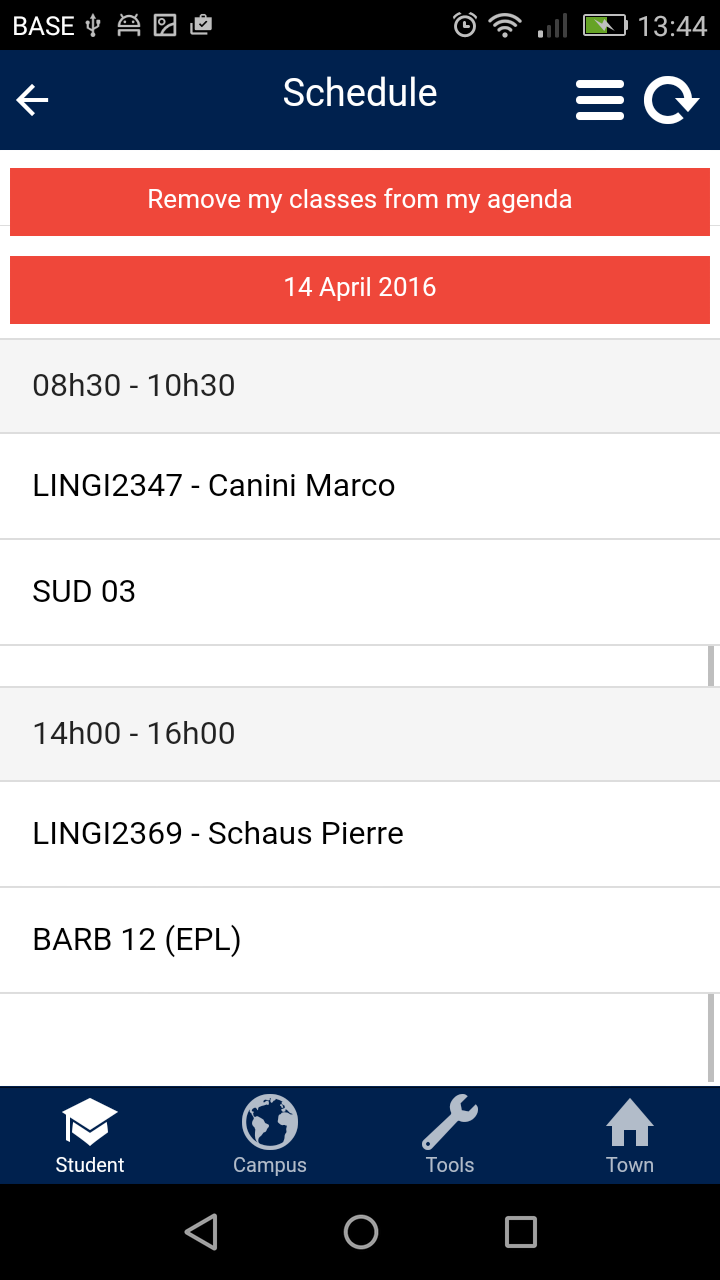
\includegraphics[width=\textwidth]{Images/Application_screens/Screenshot_2016-06-06-13-44-12.png}
    \end{subfigure}
    ~ %add desired spacing between images, e. g. ~, \quad, \qquad, \hfill etc. 
      %(or a blank line to force the subfigure onto a new line)
    \begin{subfigure}[b]{0.3\textwidth}
        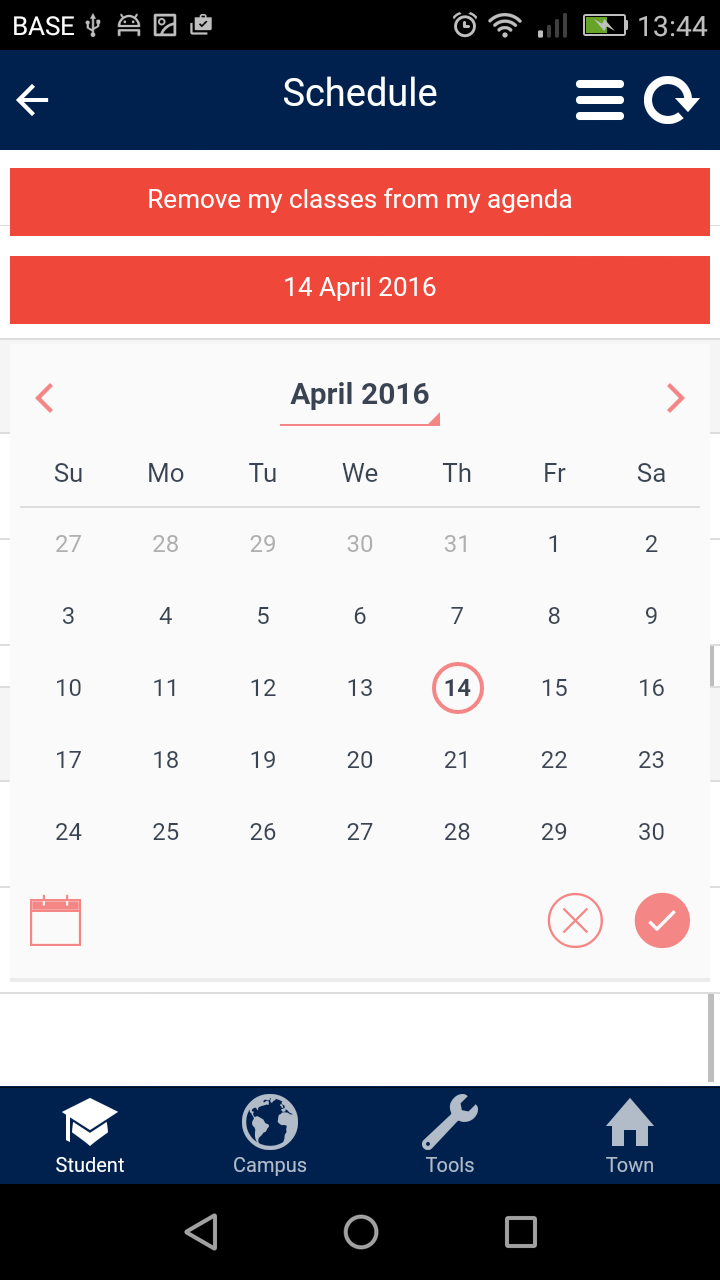
\includegraphics[width=\textwidth]{Images/Application_screens/Screenshot_2016-06-06-13-44-26.png}
    \end{subfigure}
    ~ %add desired spacing between images, e. g. ~, \quad, \qquad, \hfill etc. 
    %(or a blank line to force the subfigure onto a new line)
    \begin{subfigure}[b]{0.3\textwidth}
        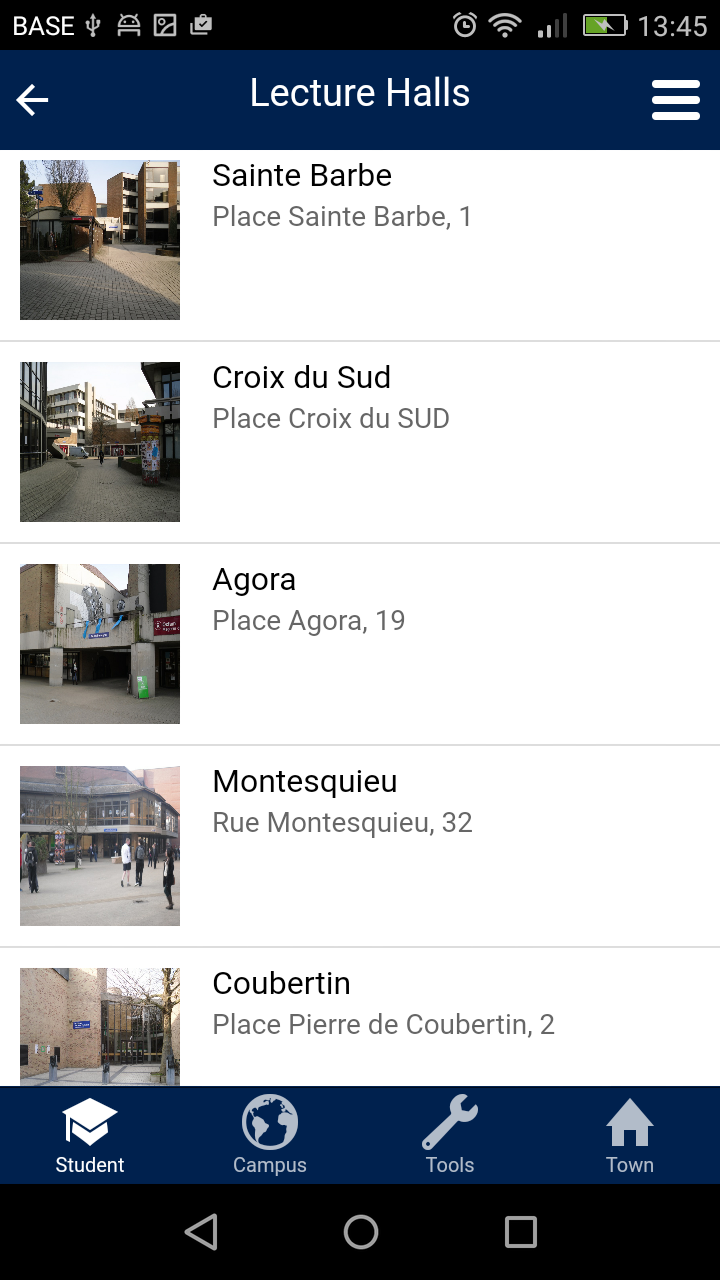
\includegraphics[width=\textwidth]{Images/Application_screens/Screenshot_2016-06-06-13-45-05.png}
    \end{subfigure}
\end{figure}
\begin{figure}
    \centering
\begin{subfigure}[b]{0.3\textwidth}
        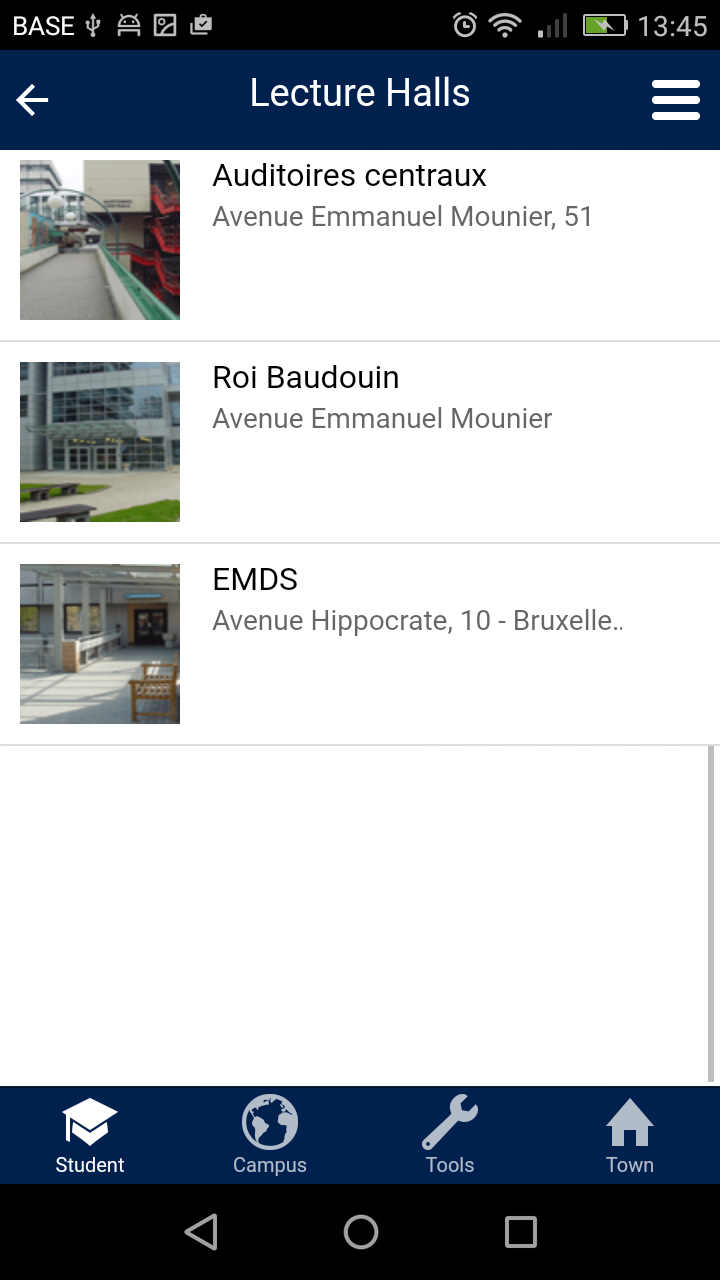
\includegraphics[width=\textwidth]{Images/Application_screens/Screenshot_2016-06-06-13-45-20.png}
    \end{subfigure}
    ~ %add desired spacing between images, e. g. ~, \quad, \qquad, \hfill etc. 
      %(or a blank line to force the subfigure onto a new line)
    \begin{subfigure}[b]{0.3\textwidth}
        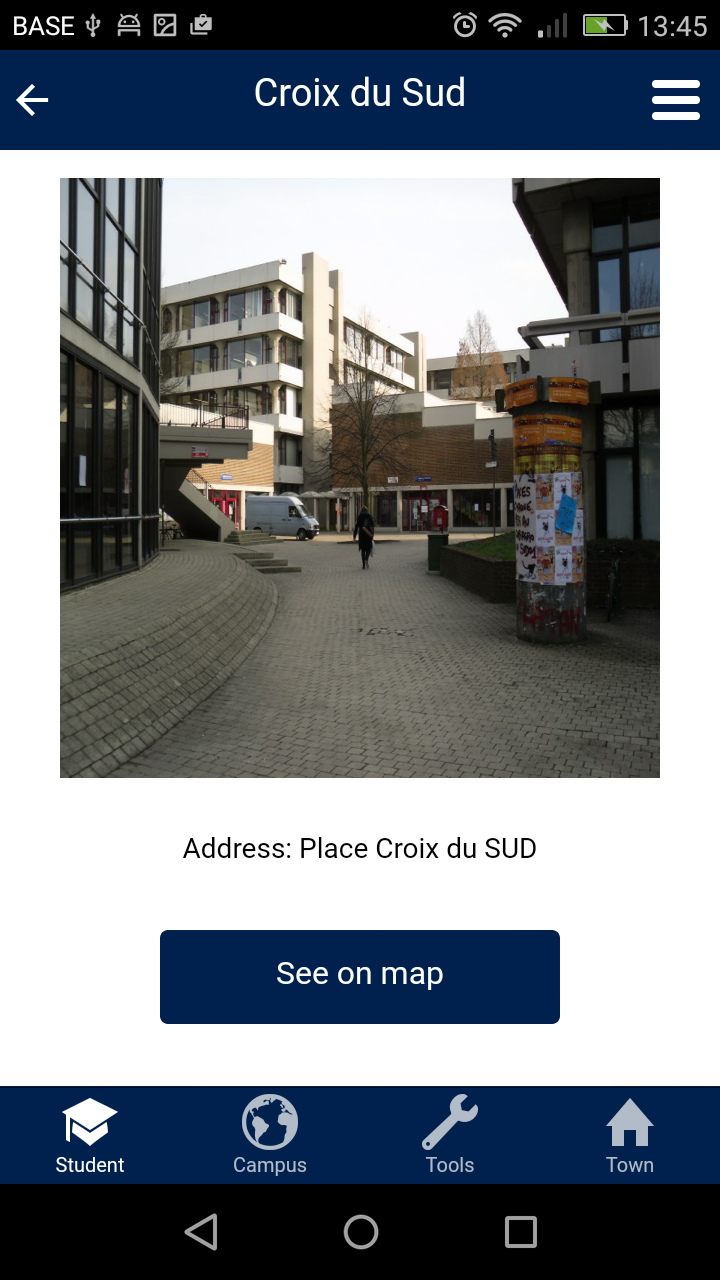
\includegraphics[width=\textwidth]{Images/Application_screens/Screenshot_2016-06-06-13-45-51.png}
    \end{subfigure}
    \begin{subfigure}[b]{0.3\textwidth}
        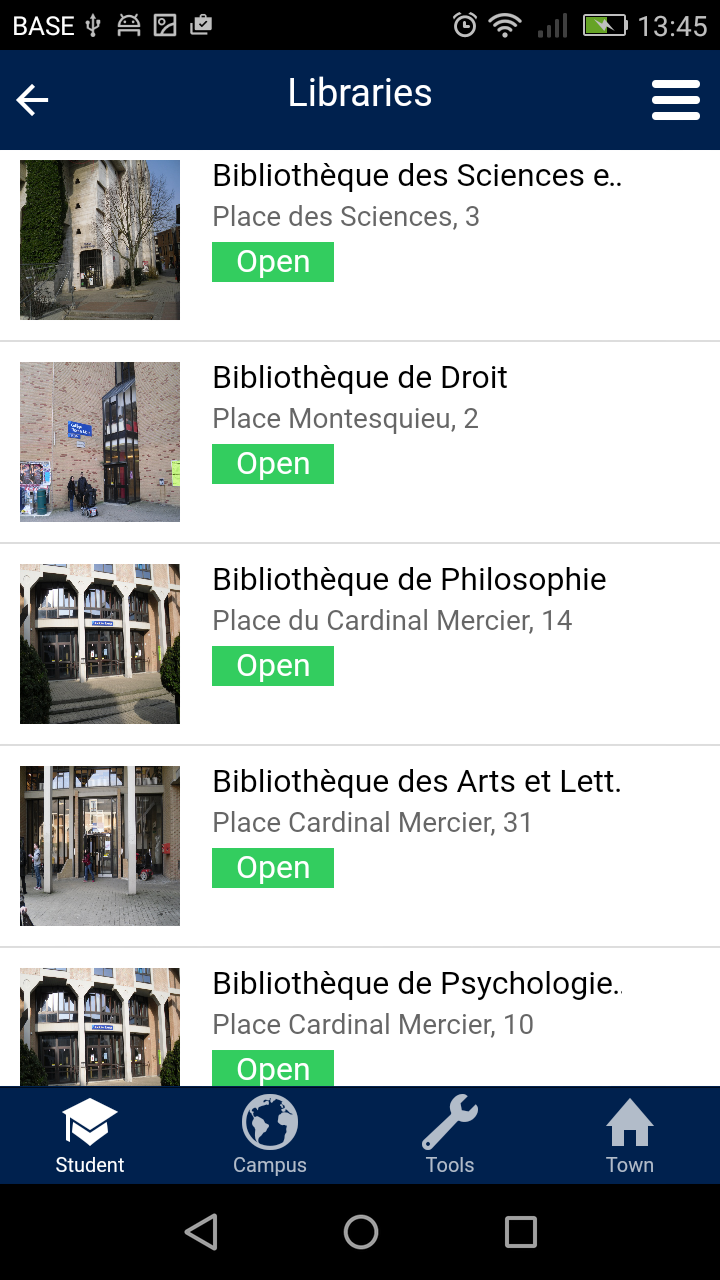
\includegraphics[width=\textwidth]{Images/Application_screens/Screenshot_2016-06-06-13-45-37.png}
    \end{subfigure}
    ~ %add desired spacing between images, e. g. ~, \quad, \qquad, \hfill etc. 
    %(or a blank line to force the subfigure onto a new line)

\end{figure}
\begin{figure}
    \centering
\begin{subfigure}[b]{0.3\textwidth}
        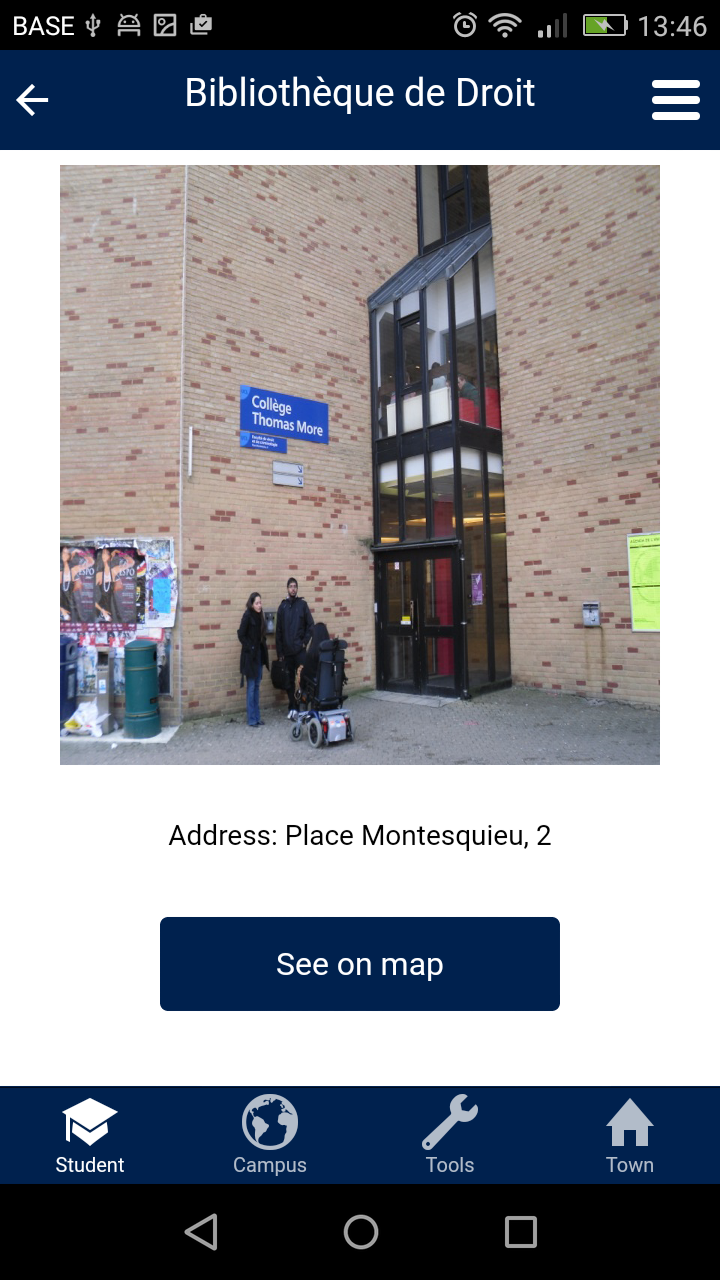
\includegraphics[width=\textwidth]{Images/Application_screens/Screenshot_2016-06-06-13-46-04.png}
    \end{subfigure}
    ~ %add desired spacing between images, e. g. ~, \quad, \qquad, \hfill etc. 
      %(or a blank line to force the subfigure onto a new line)
    \begin{subfigure}[b]{0.3\textwidth}
        
\includegraphics[width=\textwidth]{Images/Application_screens/Screenshot_2016-06-06-13-46-46.png}
    \end{subfigure}
    ~ %add desired spacing between images, e. g. ~, \quad, \qquad, \hfill etc. 
    %(or a blank line to force the subfigure onto a new line)
    \begin{subfigure}[b]{0.3\textwidth}
        
\includegraphics[width=\textwidth]{Images/Application_screens/Screenshot_2016-06-06-13-46-56.png}
    \end{subfigure}
\end{figure}
\begin{figure}
    \centering
\begin{subfigure}[b]{0.3\textwidth}
        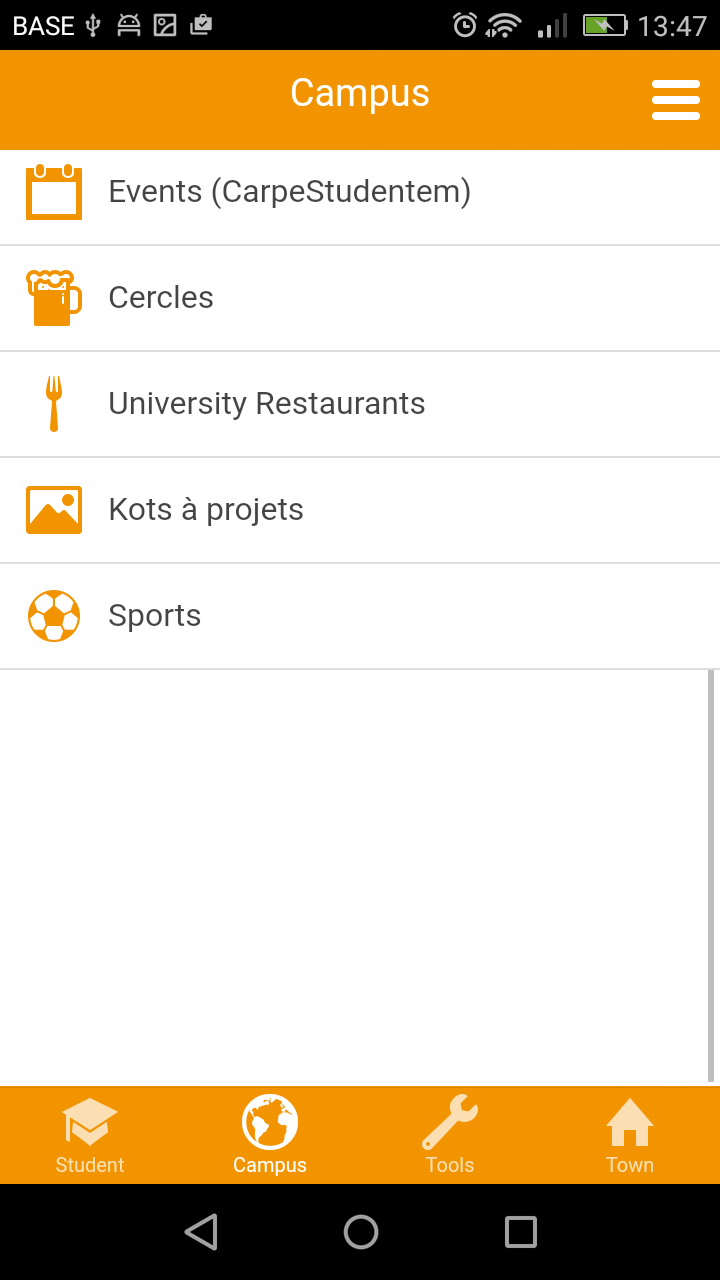
\includegraphics[width=\textwidth]{Images/Application_screens/Screenshot_2016-06-06-13-47-05.png}
    \end{subfigure}
    ~ %add desired spacing between images, e. g. ~, \quad, \qquad, \hfill etc. 
      %(or a blank line to force the subfigure onto a new line)
    \begin{subfigure}[b]{0.3\textwidth}
        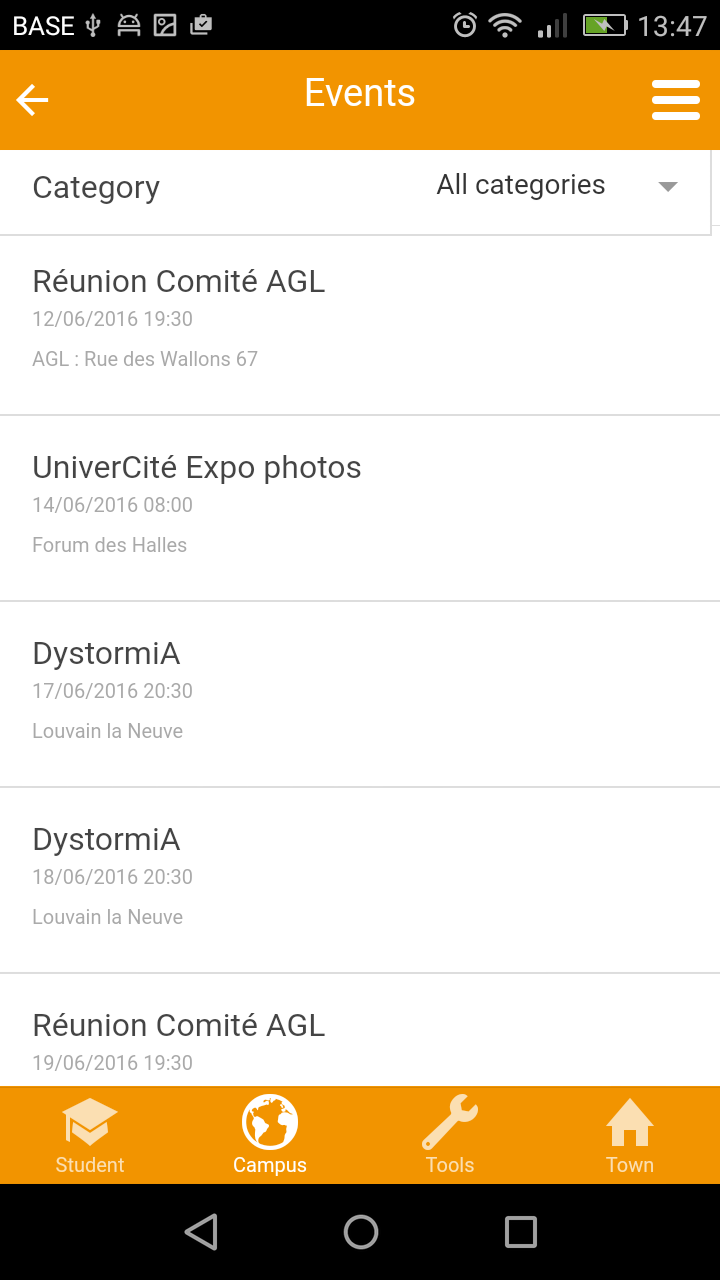
\includegraphics[width=\textwidth]{Images/Application_screens/Screenshot_2016-06-06-13-47-19.png}
    \end{subfigure}
    ~ %add desired spacing between images, e. g. ~, \quad, \qquad, \hfill etc. 
    %(or a blank line to force the subfigure onto a new line)
    \begin{subfigure}[b]{0.3\textwidth}
        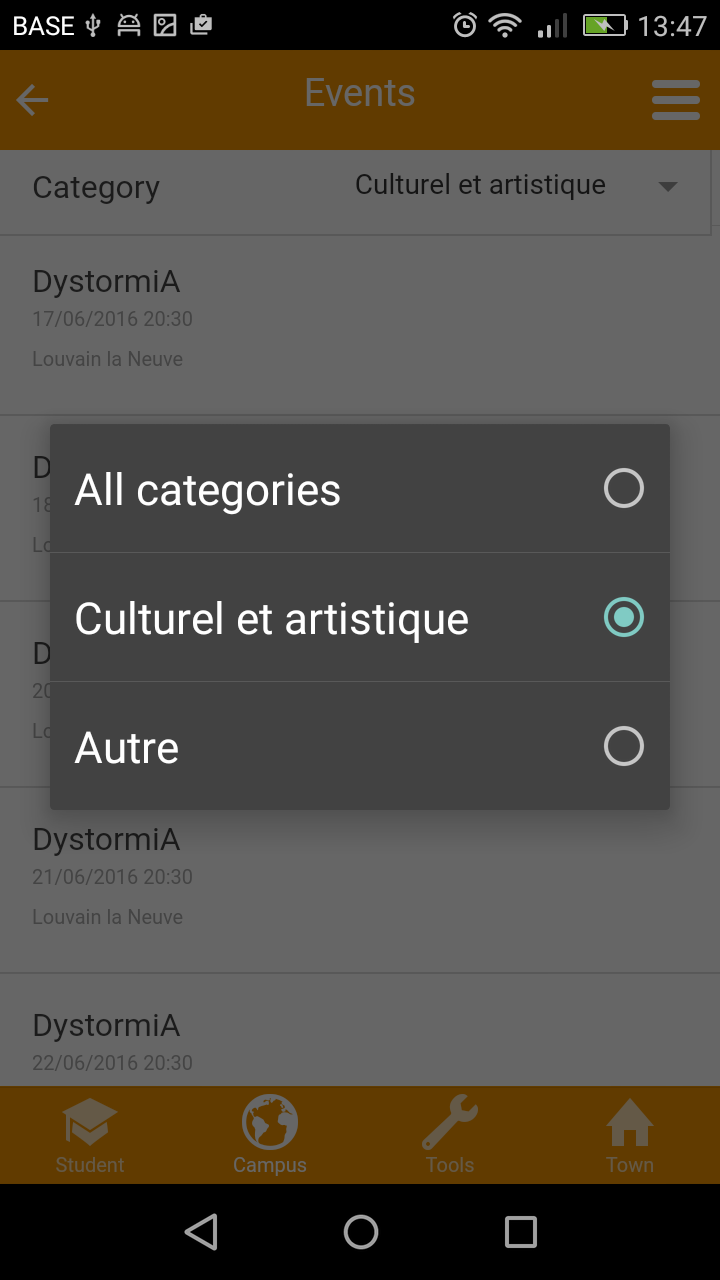
\includegraphics[width=\textwidth]{Images/Application_screens/Screenshot_2016-06-06-13-47-47.png}
    \end{subfigure}
\end{figure}
\begin{figure}
    \centering
\begin{subfigure}[b]{0.3\textwidth}
        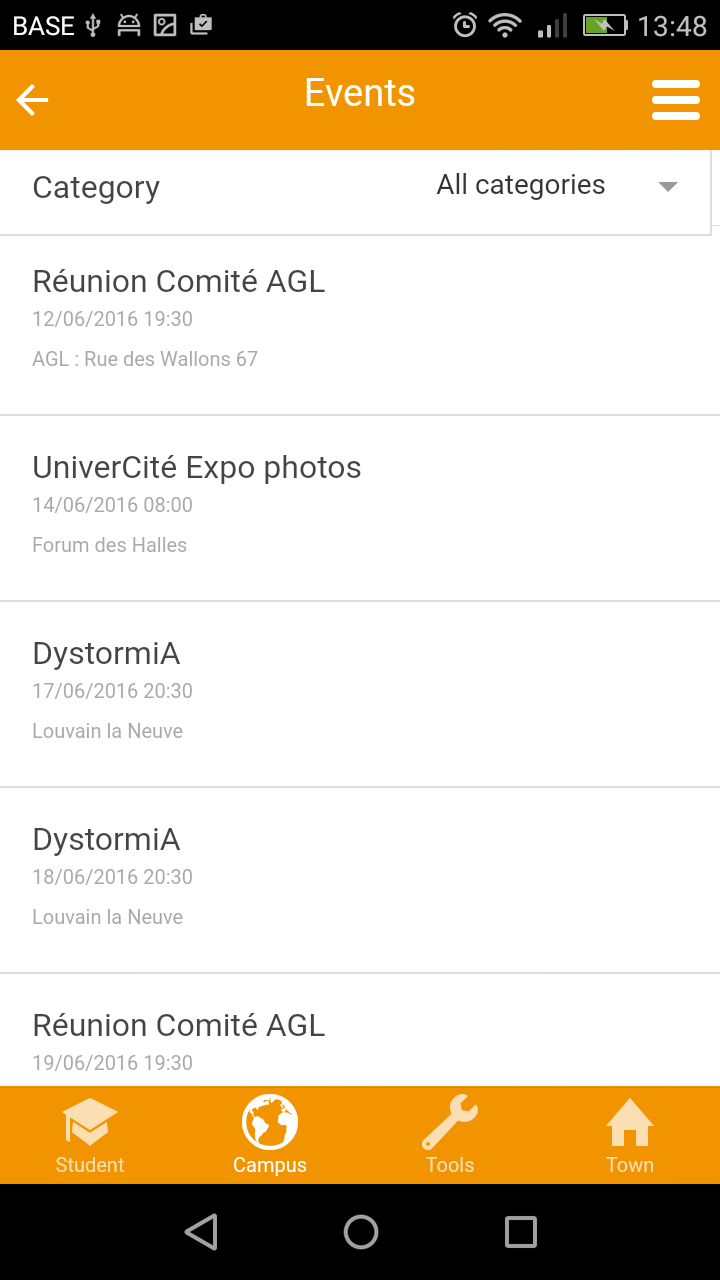
\includegraphics[width=\textwidth]{Images/Application_screens/Screenshot_2016-06-06-13-48-01.png}
    \end{subfigure}
    ~ %add desired spacing between images, e. g. ~, \quad, \qquad, \hfill etc. 
      %(or a blank line to force the subfigure onto a new line)
    \begin{subfigure}[b]{0.3\textwidth}
        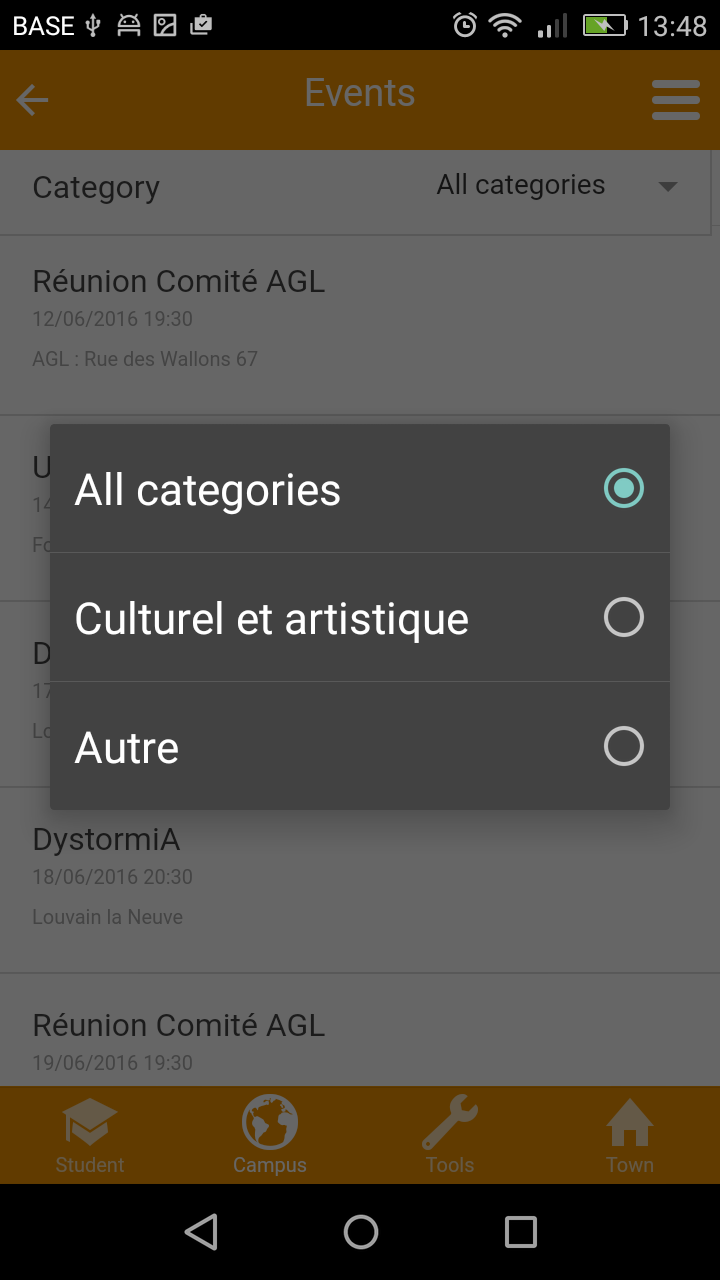
\includegraphics[width=\textwidth]{Images/Application_screens/Screenshot_2016-06-06-13-48-08.png}
    \end{subfigure}
    ~ %add desired spacing between images, e. g. ~, \quad, \qquad, \hfill etc. 
    %(or a blank line to force the subfigure onto a new line)
    \begin{subfigure}[b]{0.3\textwidth}
        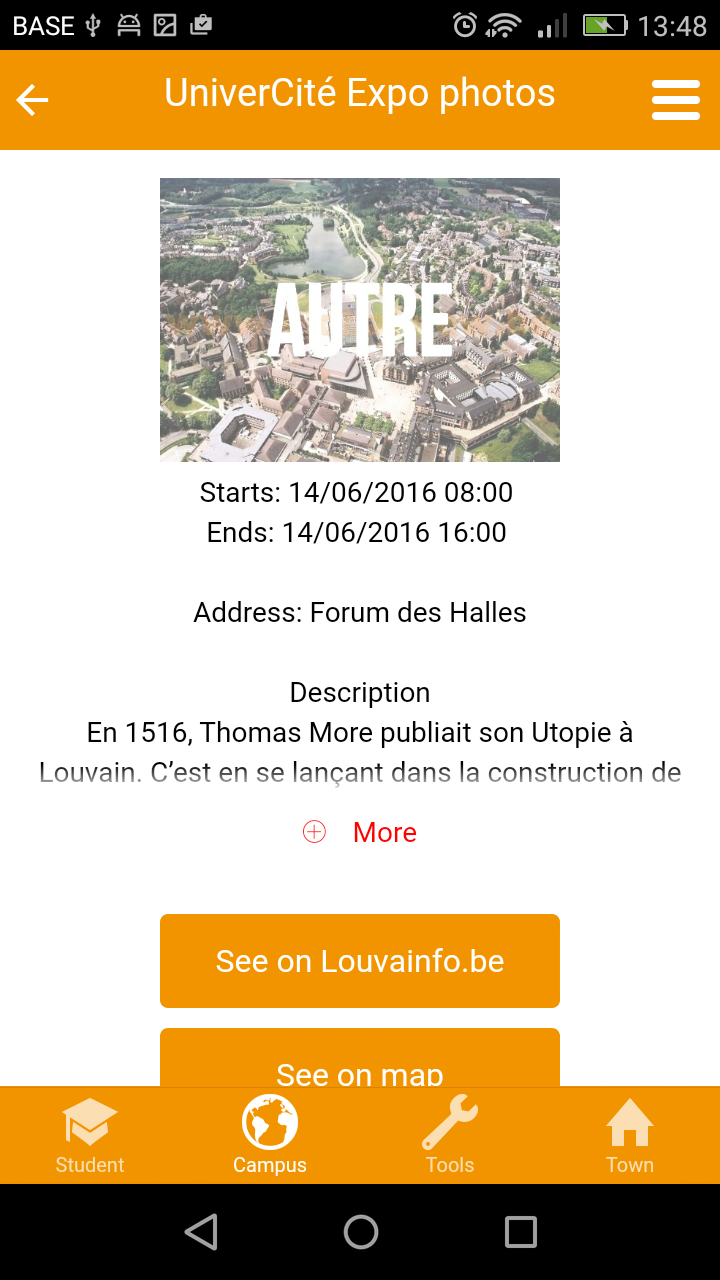
\includegraphics[width=\textwidth]{Images/Application_screens/Screenshot_2016-06-06-13-48-21.png}
    \end{subfigure}
\end{figure}
\begin{figure}
    \centering
\begin{subfigure}[b]{0.3\textwidth}
        
\includegraphics[width=\textwidth]{Images/Application_screens/Screenshot_2016-06-06-13-48-40.png}
    \end{subfigure}
    ~ %add desired spacing between images, e. g. ~, \quad, \qquad, \hfill etc. 
      %(or a blank line to force the subfigure onto a new line)
    \begin{subfigure}[b]{0.3\textwidth}
        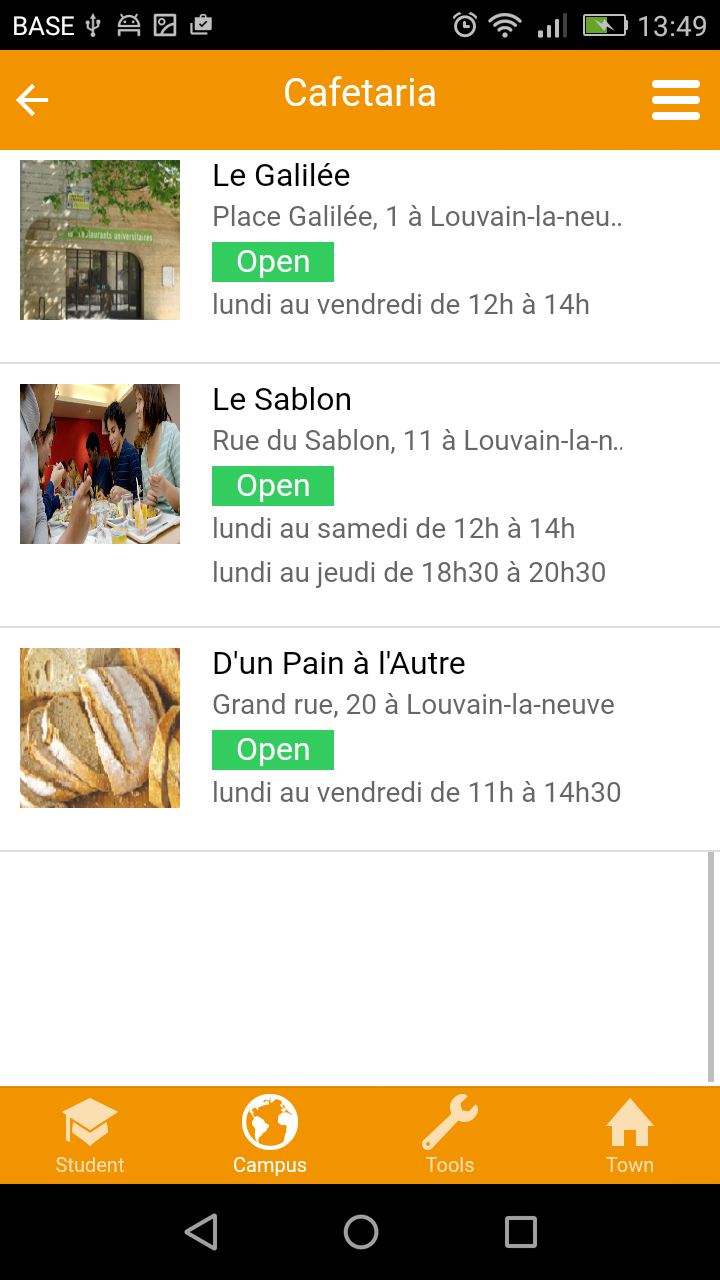
\includegraphics[width=\textwidth]{Images/Application_screens/Screenshot_2016-06-06-13-49-08.png}
    \end{subfigure}
    ~ %add desired spacing between images, e. g. ~, \quad, \qquad, \hfill etc. 
    %(or a blank line to force the subfigure onto a new line)
    \begin{subfigure}[b]{0.3\textwidth}
        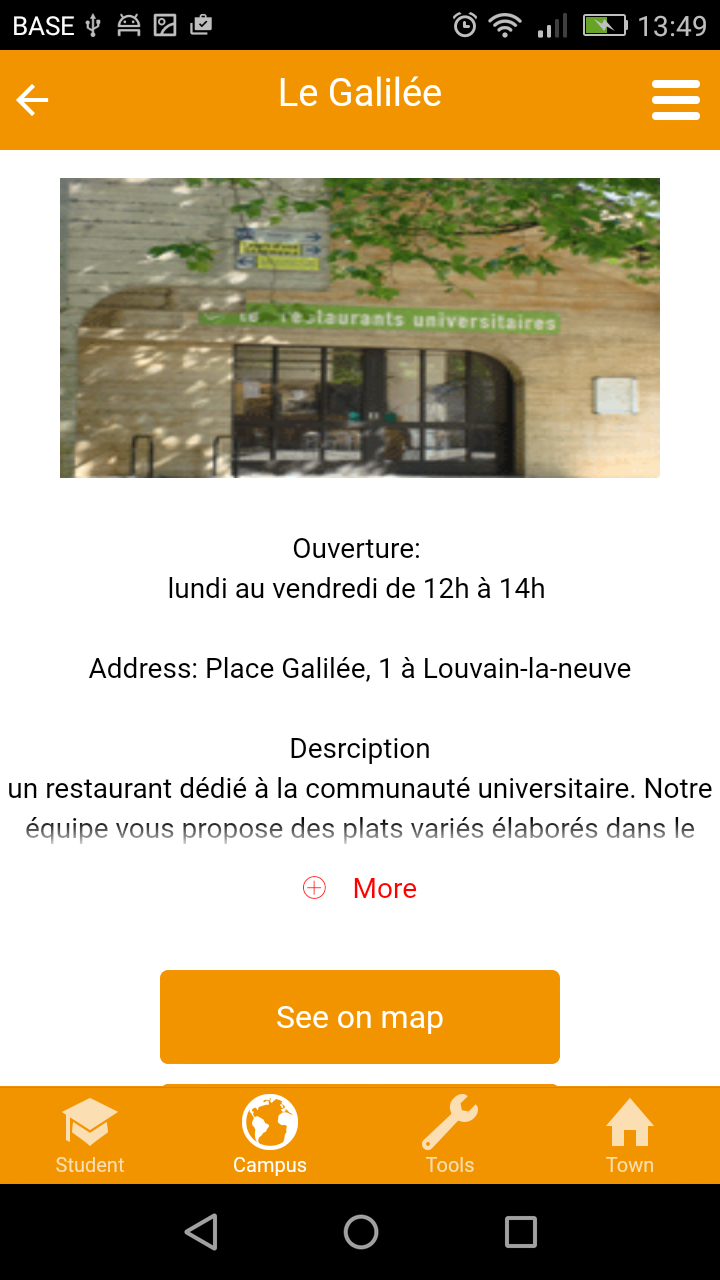
\includegraphics[width=\textwidth]{Images/Application_screens/Screenshot_2016-06-06-13-49-21.png}
    \end{subfigure}
\end{figure}
\begin{figure}
    \centering
\begin{subfigure}[b]{0.3\textwidth}
        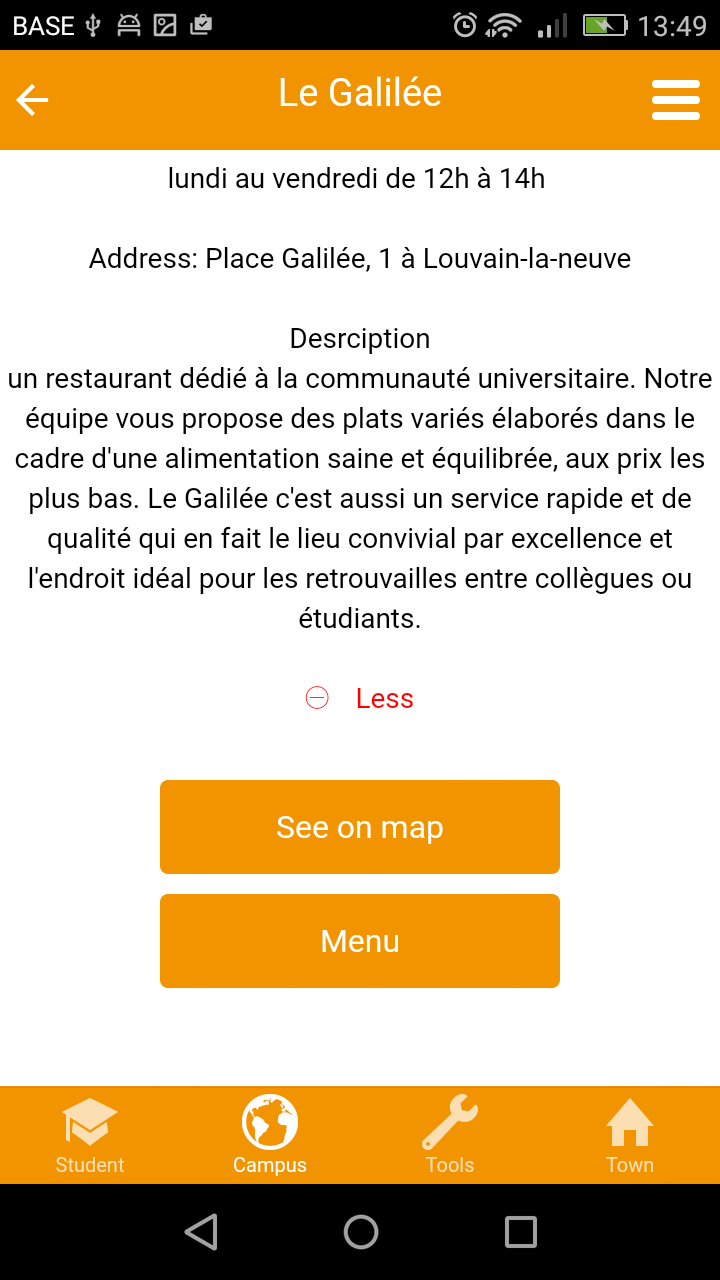
\includegraphics[width=\textwidth]{Images/Application_screens/Screenshot_2016-06-06-13-49-30.png}
    \end{subfigure}
    ~ %add desired spacing between images, e. g. ~, \quad, \qquad, \hfill etc. 
      %(or a blank line to force the subfigure onto a new line)
    \begin{subfigure}[b]{0.3\textwidth}
        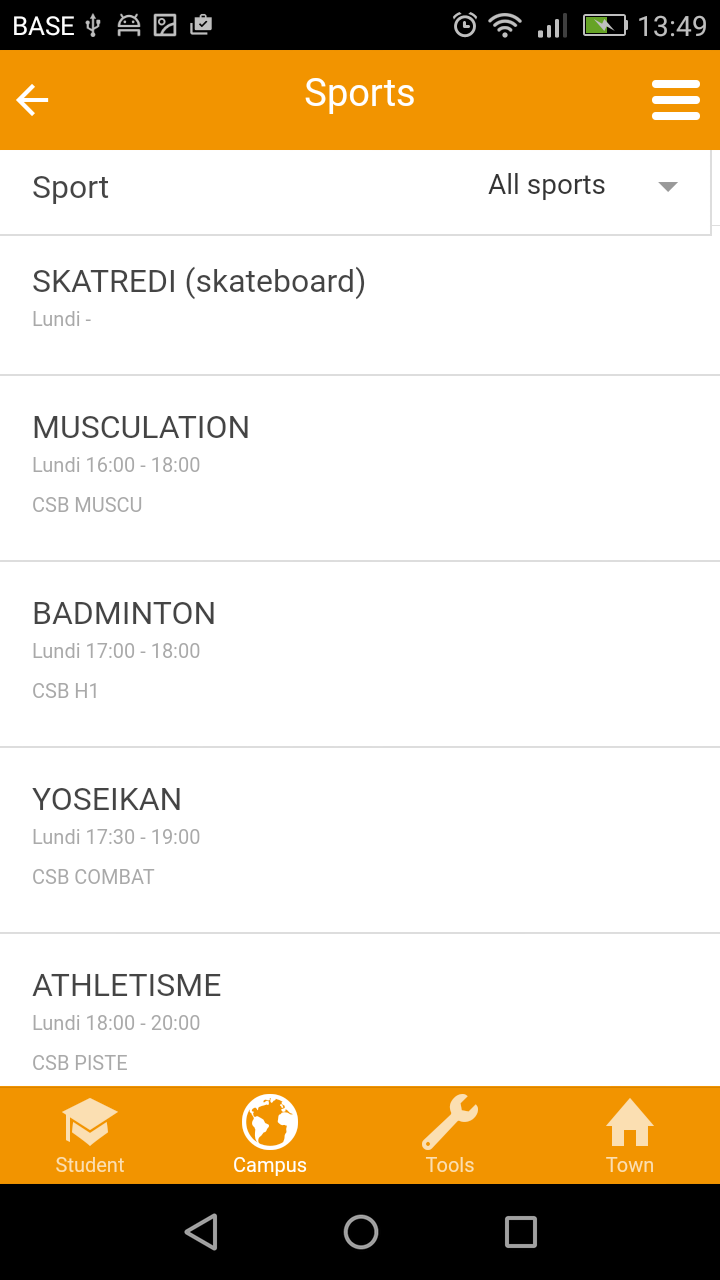
\includegraphics[width=\textwidth]{Images/Application_screens/Screenshot_2016-06-06-13-49-46.png}
    \end{subfigure}
    ~ %add desired spacing between images, e. g. ~, \quad, \qquad, \hfill etc. 
    %(or a blank line to force the subfigure onto a new line)
    \begin{subfigure}[b]{0.3\textwidth}
        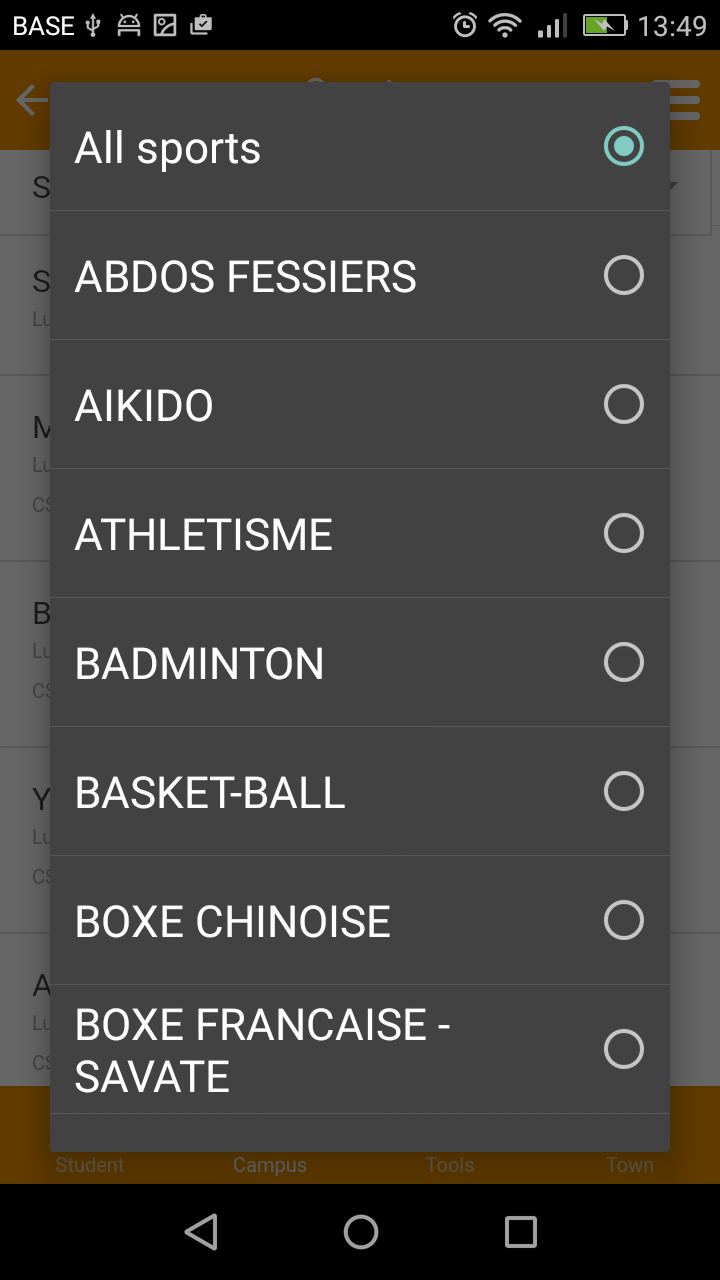
\includegraphics[width=\textwidth]{Images/Application_screens/Screenshot_2016-06-06-13-49-55.png}
    \end{subfigure}
\end{figure}
\begin{figure}
    \centering
\begin{subfigure}[b]{0.3\textwidth}
        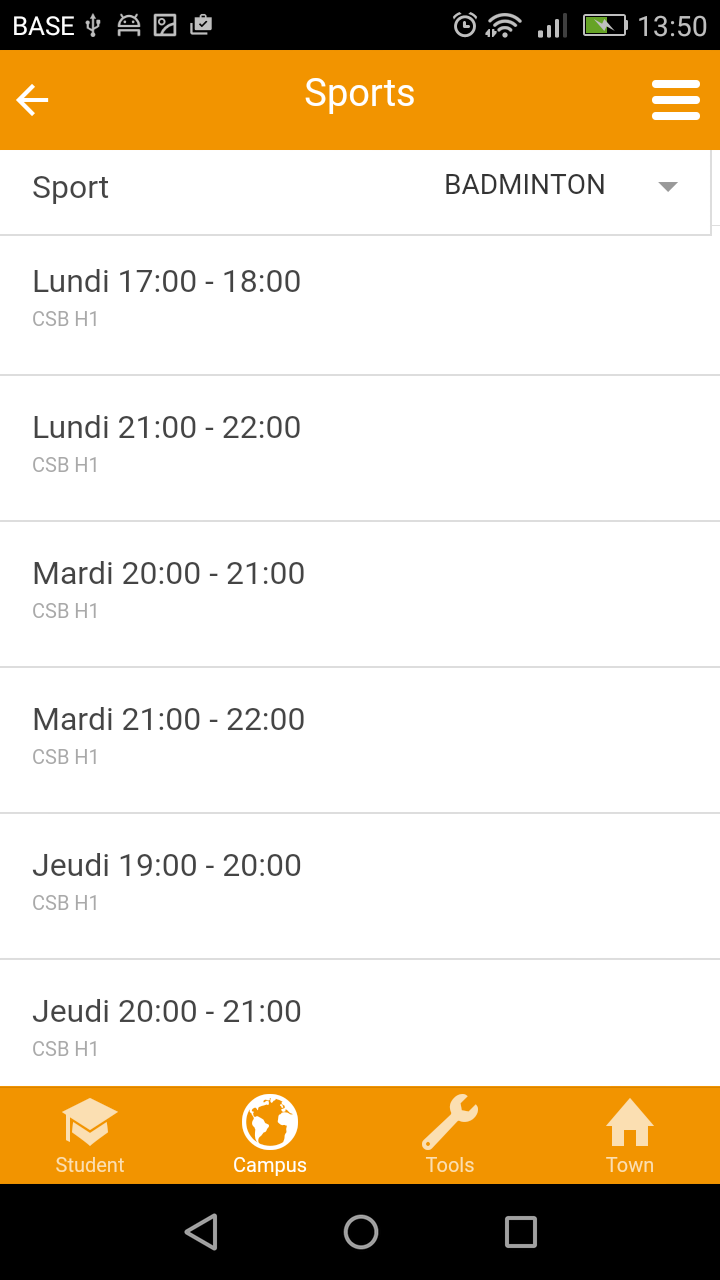
\includegraphics[width=\textwidth]{Images/Application_screens/Screenshot_2016-06-06-13-50-02.png}
    \end{subfigure}
    ~ %add desired spacing between images, e. g. ~, \quad, \qquad, \hfill etc. 
      %(or a blank line to force the subfigure onto a new line)
    \begin{subfigure}[b]{0.3\textwidth}
        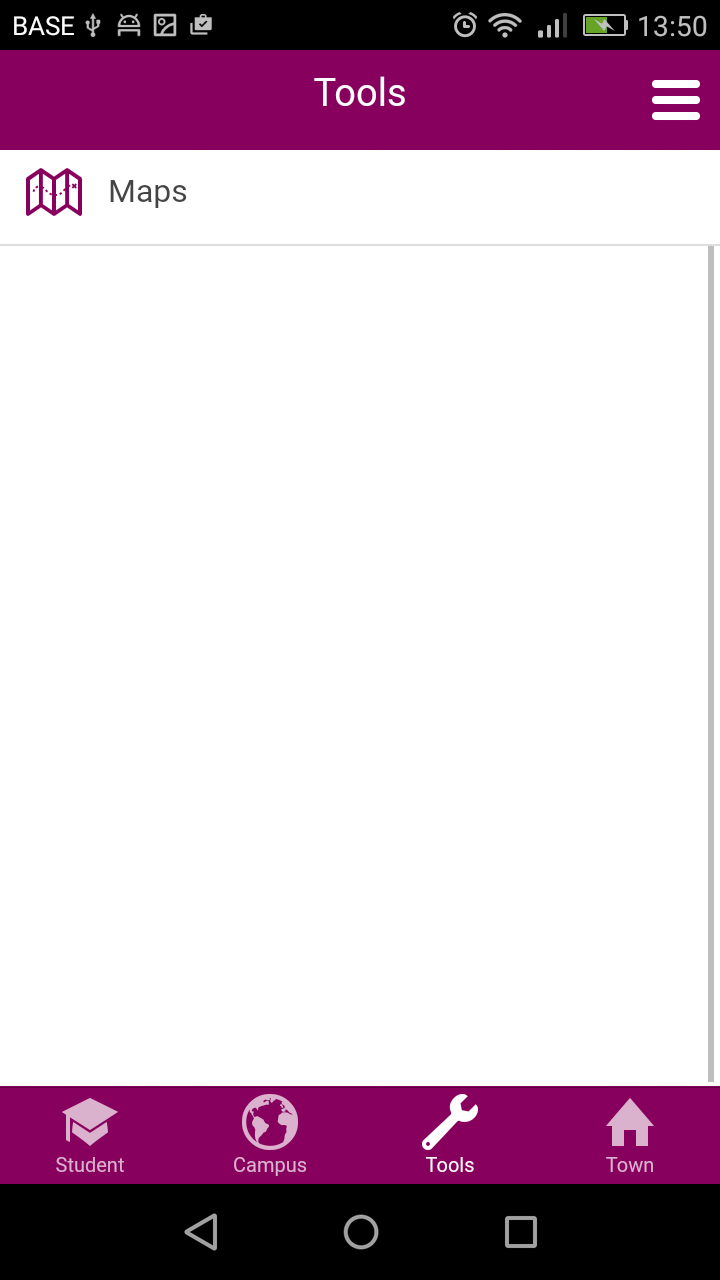
\includegraphics[width=\textwidth]{Images/Application_screens/Screenshot_2016-06-06-13-50-14.png}
    \end{subfigure}
    ~ %add desired spacing between images, e. g. ~, \quad, \qquad, \hfill etc. 
    %(or a blank line to force the subfigure onto a new line)
    \begin{subfigure}[b]{0.3\textwidth}
        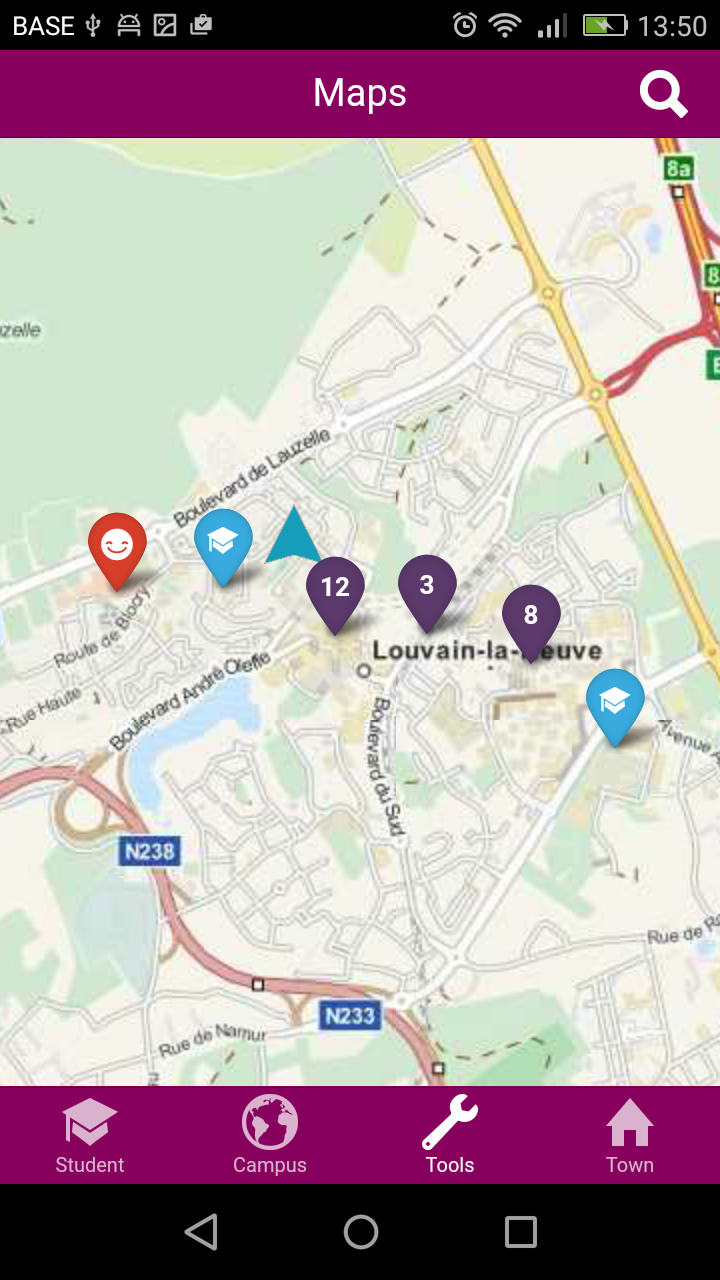
\includegraphics[width=\textwidth]{Images/Application_screens/Screenshot_2016-06-06-13-50-28.png}
    \end{subfigure}
\end{figure}
\begin{figure}
    \centering
\begin{subfigure}[b]{0.3\textwidth}
        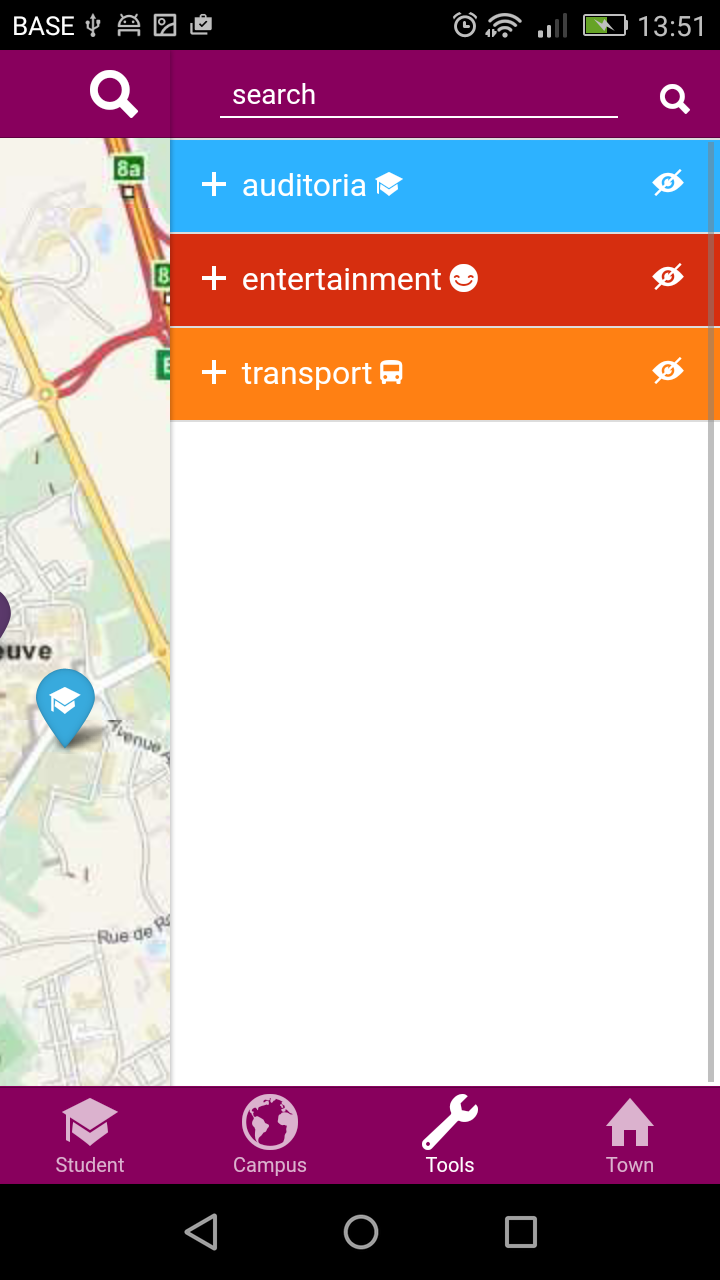
\includegraphics[width=\textwidth]{Images/Application_screens/Screenshot_2016-06-06-13-51-21.png}
    \end{subfigure}
    ~ %add desired spacing between images, e. g. ~, \quad, \qquad, \hfill etc. 
      %(or a blank line to force the subfigure onto a new line)
    \begin{subfigure}[b]{0.3\textwidth}
        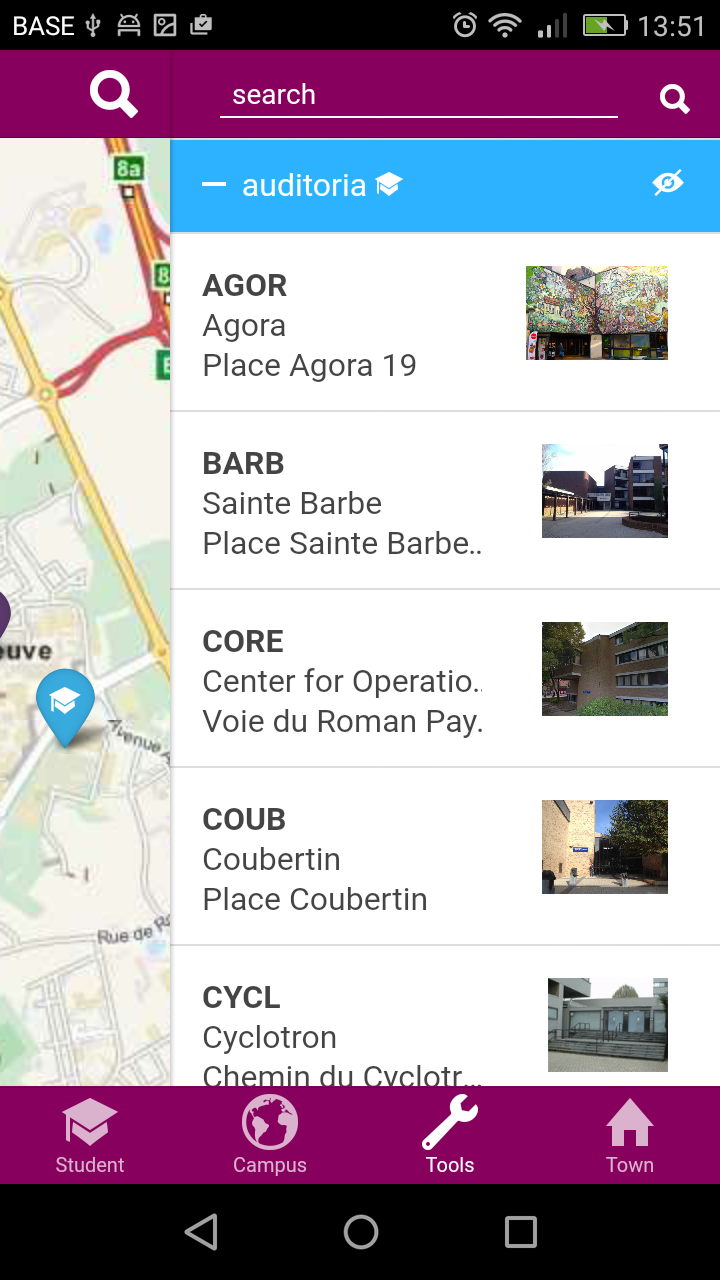
\includegraphics[width=\textwidth]{Images/Application_screens/Screenshot_2016-06-06-13-51-29.png}
    \end{subfigure}
    ~ %add desired spacing between images, e. g. ~, \quad, \qquad, \hfill etc. 
    %(or a blank line to force the subfigure onto a new line)
    \begin{subfigure}[b]{0.3\textwidth}
        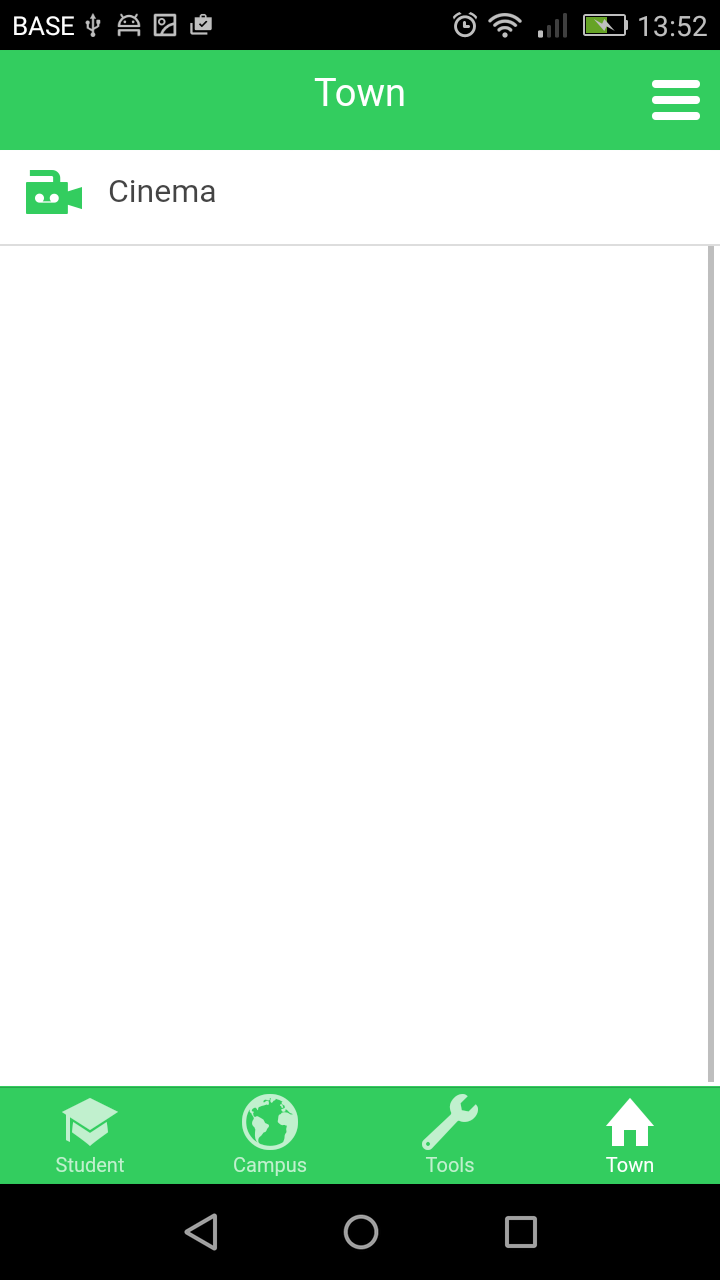
\includegraphics[width=\textwidth]{Images/Application_screens/Screenshot_2016-06-06-13-52-44.png}
    \end{subfigure}
\end{figure}


\chapter{Performance Measurements}



% Back cover page
\backcoverpage

\end{document}
